% !TEX TS-program = pdflatex
% !TEX encoding = UTF-8 Unicode

% This is a simple template for a LaTeX document using the "article" class.
% See "book", "report", "letter" for other types of document.

\documentclass[11pt,twoside]{book} % use larger type; default would be 10pt


\raggedright
\usepackage[utf8]{inputenc} % set input encoding (not needed with XeLaTeX)

%%% Examples of Article customizations
% These packages are optional, depending whether you want the features they provide.
% See the LaTeX Companion or other references for full information.

%%% PAGE DIMENSIONS
\usepackage[margin=2in,headheight=26pt]{geometry}   % to change the page dimensions
\geometry{letterpaper}  % or letterpaper (US) or a5paper or....
% \geometry{margin=2in} % for example, change the margins to 2 inches all round
% \geometry{landscape}  % set up the page for landscape
%   read geometry.pdf for detailed page layout information

\newcommand{\plogo}{\fbox{$\mathcal{PL}$}} % Generic dummy publisher logo

\usepackage{graphicx} % support the \includegraphics command and options
%\usepackage{svg-inkscape}
%\usepackage{svg}
\usepackage{bussproofs}
\usepackage{algorithm}
\usepackage{algorithmicx}
\usepackage{algpseudocode}


 \usepackage[parfill]{parskip} % Activate to begin paragraphs with an empty line rather than an indent

%%% PACKAGES
\usepackage{booktabs} % for much better looking tables
\usepackage{array}    % for better arrays (eg matrices) in maths
\usepackage{paralist} % very flexible & customisable lists (eg. enumerate/itemize, etc.)
\usepackage{verbatim} % adds environment for commenting out blocks of text & for better verbatim
\usepackage{subfig}   % make it possible to include more than one captioned figure/table in a single float
% These packages are all incorporated in the memoir class to one degree or another...

%Fonts
\usepackage[T1]{fontenc} % Output font encoding for international characters
\usepackage{fouriernc} % Use the New Century Schoolbook font

% Packages needed to set discrete math symbols 
\usepackage {amsfonts} % gives mathbb
\usepackage {amssymb}  % gives nmid (does not divide)
\usepackage {amsmath}  % to get text in math mode
\usepackage {amsthm}


% Packages to improve formatting
\usepackage {enumitem}
\usepackage {mathtools}   % for vdotswithin

%% Theorems, Definitions, Corrolaries, etc
\theoremstyle {definition}
\newtheorem {definition}{Def}[section]
\newtheorem {theorem}{Theorem}[section]
\newtheorem {corollary}{Corollary}[section]
\newtheorem{lemma}{Lemma}[section]
\newtheorem{example}{Example}
\theoremstyle {remark}
\newtheorem*{notes}{Notes}

%% Graphics, Illustrations, etc
\usepackage {graphics}
\graphicspath{ {illustrations/} }

%%% HEADERS & FOOTERS
\usepackage{fancyhdr} % This should be set AFTER setting up the page geometry
\pagestyle{fancy} % options: empty , plain , fancy
\fancyhf{}
\fancyhead[RO]{An Outline of Discrete Mathematics}
\fancyhead[LE]{\rightmark}
\fancyfoot[LE]{\thepage}
\fancyfoot[RO]{\thepage}
\renewcommand{\headrulewidth}{0pt} % customise the layout...


%%% SECTION TITLE APPEARANCE
\usepackage{sectsty}

\allsectionsfont{\sffamily\mdseries\upshape} % (See the fntguide.pdf for font help)
% (This matches ConTeXt defaults)

\usepackage[compact]{titlesec}
\titlespacing{\section}{0pt}{*4}{*0}
%\titlespaceing{\subsection}{0pt}{*4}{*0}

%%% ToC (table of contents) APPEARANCE
\usepackage[nottoc,notlof,notlot]{tocbibind}

 % Put the bibliography in the ToC
\usepackage[titles,subfigure]{tocloft}                  % Alter the style of the Table of Contents
\renewcommand{\cftsecfont}{\rmfamily\mdseries\upshape}
\renewcommand{\cftsecpagefont}{\rmfamily\mdseries\upshape} % No bold!

%%%%% Indexing
\usepackage{imakeidx}

%%% END Book customizations

%%% The "real" document content comes below...
%\usepackage{xcolor}
%\definecolor{titlepagecolor}{cmyk}{1,.60,0,.40}
%\definecolor{namecolor}{cmyk}{1,.50,0,.10} 

\makeindex
\begin{document}
  \frontmatter 
	%%%%%%%%%%%%%%%%%%%%%%%%%%%%%%%%%%%%%%%%%
% Formal Book Title Page
% LaTeX Template
% Version 2.0 (23/7/17)
%
% This template was downloaded from:
% http://www.LaTeXTemplates.com
%
% Original author:
% Peter Wilson (herries.press@earthlink.net) with modifications by:
% Vel (vel@latextemplates.com)
%
% License:
% CC BY-NC-SA 3.0 (http://creativecommons.org/licenses/by-nc-sa/3.0/)
% 
% This template can be used in one of two ways:
%
% 1) Content can be added at the end of this file just before the \end{document}
% to use this title page as the starting point for your document.
%
% 2) Alternatively, if you already have a document which you wish to add this
% title page to, copy everything between the \begin{document} and
% \end{document} and paste it where you would like the title page in your
% document. You will then need to insert the packages and document 
% configurations into your document carefully making sure you are not loading
% the same package twice and that there are no clashes.
%
%%%%%%%%%%%%%%%%%%%%%%%%%%%%%%%%%%%%%%%%%



%----------------------------------------------------------------------------------------
%	TITLE PAGE
%----------------------------------------------------------------------------------------


\begin{titlepage} % Suppresses headers and footers on the title page

	\centering % Centre everything on the title page
	
	\scshape % Use small caps for all text on the title page
	
	\vspace*{\baselineskip} % White space at the top of the page
	
	%------------------------------------------------
	%	Title
	%------------------------------------------------
	
	\rule{\textwidth}{1.6pt}\vspace*{-\baselineskip}\vspace*{2pt} % Thick horizontal rule
	\rule{\textwidth}{0.4pt} % Thin horizontal rule
	
	\vspace{0.75\baselineskip} % Whitespace above the title
	
	{\LARGE A BRIEF OUTLINE\\ OF\\  ~DISCRETE MATHEMATICS\\} % Title
	
	\vspace{0.75\baselineskip} % Whitespace below the title
	
	\rule{\textwidth}{0.4pt}\vspace*{-\baselineskip}\vspace{3.2pt} % Thin horizontal rule
	\rule{\textwidth}{1.6pt} % Thick horizontal rule
	
	\vspace{2\baselineskip} % Whitespace after the title block
	
	%------------------------------------------------
	%	Subtitle
	%------------------------------------------------
	
	A Short Course in Discrete Mathematics for a Computer Science Undergraduate % Subtitle or further description
	
	\vspace*{3\baselineskip} % Whitespace under the subtitle
	
	%------------------------------------------------
	%	Editor(s)
	%------------------------------------------------
	
	Edited By
	
	\vspace{0.5\baselineskip} % Whitespace before the editors
	
	{\scshape\Large Dale Fletter \\ D P \\} % Editor list
	
	\vspace{0.5\baselineskip} % Whitespace below the editor list
	
	\textit{The University of California \\ Davis} % Editor affiliation
	
	\vfill % Whitespace between editor names and publisher logo
	
	%------------------------------------------------
	%	Publisher
	%------------------------------------------------
	
	\plogo % Publisher logo
	
	\vspace{0.3\baselineskip} % Whitespace under the publisher logo
	
	2019 % Publication year
	
	{\large publisher} % Publisher

\end{titlepage}

%----------------------------------------------------------------------------------------


% that contains    \begin{titlepage}...\end{titlepage}
        
        copyright Dale Fletter, 2018\\
        \vspace{1in}
               
       \noindent\rule{8cm}{0.4pt}

        created using \LaTeX\  via TexWorks
        © 2007-2017 Jonathan Kew, Stefan Löffler, Charlie Sharpsteen
       Version 0.6.2 (travis-ci) [r.7ecce17, 4/29/17 9:23 AM]running on a MacBook Pro under macOS Mojave, 10.14.2
       \vspace{1in}
       
       
       Für alle, die die Schönheit von Wissenschaft anderen zeigen wollen.
       
       
       
       
       \noindent\rule{8cm}{0.4pt}
	% that contains copyright, ISBN, etc.
        %\input{dedication}% saying "this book is created for my parents..." 
        %\input{Target Audience}
        %\input{author}% about the author
        %\input{editor}% about the editor
        %\setcounter{tocdepth}{1}
        \tableofcontents
        \listoffigures
        \listoftables
        %\lstlistoflistings
	
\chapter* {Introduction}
Discrete math is a survey of many different areas of mathematics not covered by the usual series of calculus classes required of an engineering student. Since it is a survey it uses an overwhelming number of conventional symbols that have been adopted over the centuries by mathematicians. You will be reading a paper that was set using a popular free typesetting tool called Latex that is nearly universally used by scientists, engineers and mathematicians to publish papers. At times in this paper you will see references to backslashed sequences like $\forall$, $\in$, etc. These are references to the plaintext markups that are used in Latex in case you want to begin using that tool. For anyone who aspires to graduate school it is a requirement.


While the intent of this material is to be as purely formal as possible, it is necessary to make the course easier to make some assumptions of prior knowledge even before it is formally introduced. For example the section on logic assumes the reader is already familiar with all secondary school math including the concepts of integer versus real numbers and the basic rules of algebra.

In order to make a course for this material as compact and efficient as possible, this outline makes many assumptions about prerequisite material. It is assumed the student is already familiar with a two column proof form as typically presented in a high school geometry class. At least two courses in programming are assumed with a thorough understanding of the logic of Boolean expressions and their evaluation. The most basic understanding of function and set are taken as a given to avoid introducing more formal material on those topics. Directed graphs are introduced when talking about relations even though the formal treatment is later. And any material which requires calculus is excluded even though the student is expected to have the algebra skills that are needed to complete at least one course in calculus requires.

For an intense 6 week summer course there is always a chance that all of the material in this outline will not be covered. In our opinion the section on discrete probability can be safely skipped when the program will require a full course in statistics and probability. And the section on trees can be skipped since there will be a programming course on data structures and the student who completes this section on graphs should be well prepared to quickly master the new material in that course. An instructor using this material can of course take the chapters in a different order although there was great attention given this outline to avoid introducing material out of this sequence. 

\section*{Comment About Copyright}
This text must be treated as a derivative work of Rosen unless and until a publisher picks up this manuscript. I believe that it can be used under a theory of fair use for classroom use but that is not a legal opinion, only a self-serving moralistic one. I would encourage anyone who wishes to use this consider the policies of their institution before making copies readily available. 

\section*{Comments About the Order of the Material}
There are two ways to approach this material in the courses I have seen, start with logic or start with sets. I believe that starting with logic makes more sense for two reasons. First, a computer science student will have already achieved a level of mastery over Boolean expressions from programming and will be comfortable with the introduction of propositional calculus. Second, for those who wish to take a more formal approach to the material, they can get through the section on logic and may be able to largely skip the section on proofs and achieve that end. To make this text more approachable for those at a teaching college we have chosen to cover logic first to make the discussion of proofs easier.

Many instructors like to introduce relations before functions and in many academic ways it makes more sense. However every student has been well introduced to functions before they take this course but only introduced to relations in a less rigorous way. By giving them material that they think they know but developing a more formal approach to it, the fact that relations can be viewed as a superset of functions should make it easier for them to grasp the formalism. 

Many instructors will place the material on Graphs and Trees at the end of the course. We believe this is a mistake. Material covered at the end of the course is often neglected and the applications of graphs and trees are essential in industry and in later computer science courses. We bring it forward to ensure that there is sufficient time to study them in depth. This is done to the detriment of discrete probability. We believe that every computer science program will require a course in probability and statistics and find that putting this material at the end does not impact the flow of presentation while recognizing the value of giving a student some exposure to the discrete form of probability before that undergraduate material. 

We use a similar reason to push the material on computation to the end. Many courses do not even take up this subject in favor of covering it as a complete course by itself. We include it here to offer some flexibility to the instructor who may choose to cover some material without trying to cover all the material we provide. 

We intend for this text to be a competitor to Schaum's Outline which we have judged to be insufficient for our course offerings. This text has far greater depth than Schaums's requiring less supplementation for the instructor. 

\section* {Stylistic and typographic quirks}
Style manuals specify that a period at the end of a sentence be included within the parenthetic expression when it ends the sentence. We reject that and go with the non-standard usage of placing the period after the closing parethesis. Likewise for quotes, commas, etc. The attempt is to bring the English into alignment with programming practice instead of obedience to an illogical (from a CS perspective) convention.

\section*{Some History}
Previous to the 1970s, there were no computer science programs to speak of. Those who were the computer science pioneers were mathematicians first and practiced computer science as applied mathematics. Consequently they were well educated in many areas of mathematics that are truncated or absent in many computer science programs as the major tends to cater more toward the needs of software engineers instead of applied mathematicians. 

At its best, a course in discrete mathematics for the computer scientist must cover a great deal of material in a very short period of time. This is compounded by its placement in most programs in the first two years of undergraduate study. The need to teach it quickly and thoroughly is a challenge. This particular text was originally created to serve as a reference text to replace dependence upon Schaum's or one of the many texts offered. In our opinion those texts suffered from one of two defects, they were either encyclopedic and expensive or they left out key material that required supplementation by the instructor. This text at least answers the second problem and arguably the first in some applications. By reducing the exercises and most of the proofs for the theorems it is far shorter than the scope of material would allow if it attempted to take on the burden of being a teaching text. So it still requires a great deal of supplement for exercises and lectures. However for a student reference work to use during and after the course we believe it is superior to any alternative. And of course it is being offered for free to fellow instructors of this material. The assumption is that some instructors, and perhaps even some students, will offer constructive criticism on how the mission of this text can be improved for future instructors and students.

It may seem a bit pompous to call this a forward to the first edition. But that is simply done to acknowledge that as a first edition this text is surely imperfect in many ways. Most obviously there are inevitable typographical errors from transcription or flaws in the language. But it is also a hope that we will return to this and offer other volumes connected to this which include the much needed exercises and even some courseware to make the job of an instructor charged with teaching this material slightly easier.


  \mainmatter

	                         %%%   LOGIC   %%%
\chapter {Logic}
Logic is foundational for all of science and math. For computer science it is important to recall that most computers are logic machines. While logic can be studied using language, as was the liberal arts tradition, we abstract away the language and deal with a pure symbolic logic and that will be our focus. Since you are already well familar with how to construct Boolean expressions in some programming language we expect you will easily understand the development. Your instructor introduce the fascinating subject of natural language to the strict symbolic language forms in lecture and/or exercises. We will use this symbolic logic to prove things about any domain that can be represented using propositions and predicates.


\section {Propositional Logic}
\begin {definition}[Proposition] \index{proposition}
A proposition is a declarative sentence which is true or false, but not both. Also called a statement. In symbolic logic we use single lowercase letters beginning with p to represent propositions. These are called \textit{propositional variables}.
\end {definition}

\marginpar{A sentence with variables are not propositions. Pronouns function as variables since the antecedent of the pronoun is ambiguous.}

\begin{notes}
 There are two \textbf{literal values} in this logic, one that represents true and the other that represents false. Most commonly T is used for true and F for false. It is also common to use 1 for true and 0 for false. Many computer implementations do this, sometimes with unintended consequences. Questions (interogatives) and commands (statements in the imperative mood) are not propositions since no truth value can be associated with them. The \textbf{truth value} of a proposition is true, denoted by the logical literal T, if it is a true proposition, and the truth value of a proposition is false, denoted by F, it it is a false proposition. The area of logic that deals with propositions is called the \textbf{propositonal calculus} or \textbf{propositional logic}. 
\end{notes}

\subsection{Atomic and Compound Propositions and Logical Connectives}
\begin {definition}[Logical Connectives and Compound Propositions]\index{compound proposition}\index{logical connective}
A \textbf{compound proposition} is a proposition formed from atomic propositions with logical connectives or logical operators. Also called a logical or Boolean expression. An atomic propositions is one that is not a compound propositions.
\end {definition}

Note Schaum's represents an abstract compound proposition P with atomic propositions p,q,r, etc as P(p,q,r,...).

\begin {definition}[Negation]\index{negation}
Let $p$ be a proposition. The \textit{negation of p}, denoted by $\lnot p$ (also denoted by $\overline{p}$, is the statement 
\textit{"It is not the case that $p$."}\\
The proposition $\lnot p$ is read "not $p$". The truth value of the negation of $p$,  $\lnot p$, is the opposite of the truth value of $p$. Other notations for logical negation include $\neg$ and $\sim$. Many computer science students will use the ! symbol as well.
\end {definition} 

Note how you can always negate a natural language proposition by prepending the phrase, "it is not the case that..." followed by the original proposition.

\begin{definition}[Truth Table]\index{truth table}
Compound propositions are often presented in a table which shows the truth value associated with the expression for every possible combination of the atomic propositions in that compound proposition. The order of the rows most commonly starts with true for all atomic propositions and proceeds by alternating the rightmost atomic proposition between true and false with changes in the next leftmost proposition until all possible combinations have been listed. Table \ref{table:negation} displays the \textbf{truth table} for the negation of a proposition. The negation symbol is a unary operator taking as the single operand the proposition and giving a new propositon which is the negation of the given proposition. 
\end{definition}
    
   \begin{table}[htbp]
   \centering
   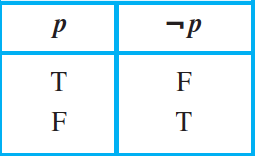
\includegraphics [width=1.5in]{Table-1-1-1-Negation}
   \caption{The Truth Table for the Negation of a Proposition}
   \label{table:negation}
   \end{table}

\begin {definition}[Conjunction]\index{conjunction}
 Let $p$ and $q$ be propositions. The \textit{conjunction} of $p$ and $q$, denoted by $ p \land q$, is the proposition \textit{p and q}. The conjunction $p \land q$ is true when both $p$ and $q$ are true and is false otherwise.
\end {definition}

\begin {definition}[Disjunction]\index{disjunction}
Let $p$ and $q$ be propositIons. The disjunction of $p$ and $q$, denoted by $p \lor q$, is the proposition \textit{p or q}. The disjunction $p \lor q$ is false when both $p$ and $q$ are false and true otherwise.
\end {definition}

Logical disjunction captures part of the meaning of the natural language word "or." But logical disjunction must be carefully observed to have a distinct formal meaning. Contrast this with what is called the exclusive or.

\begin {definition}[Exclusive OR]\index{exclusive OR}
Let p and q b propsition. The \textit{exclusive or} of $p$ and $q$, denoted by $p \oplus q$, is the proposition that is true when exactly one of $p$ and $q$ is true and is false otherwise.
\end {definition}

\subsection {Conditional Statements or Logical Implication}
\begin {definition}\index{implication}\index {antecedent}\index{conditional statement}\index{hypothesis}\index{premise}\index{conclusion}\index{consequent} 
Let $p$ and $q$ be propositions. The conditional statement $p \rightarrow $q is the proposition "if p then q".  The conditional statement $p \rightarrow q$ is false when $p$ is true and $q$ is false, and true otherwise. In the conditional statement  $p \rightarrow q$, $p$ is called the \textbf{hypothesis} (or \textbf{antecedent} or \textbf{premise})( and $q$ is called the \textbf{conclusion}, \textbf{consequent}. There are many ways in which the implication is set in type. Alternatives to what is defined here include  $\implies$ and $\supset$. It is acceptable to use -> when typing. 
\end {definition}

\begin{notes}
logical implication is not causality. When the antecedent is false the expression is always true. The only way the expression is false is when the antecedent is true and the consequence is false. \\

this is a logical operator and must not be confused with the use of the conditional statement in programmng languages. We will discuss this again in the section on Algorithms.

Conditional statements are a backbone of deductive logic and mathematical reasoning. Yet students often fail to grasp how to understand and use these statements. The lack of understanding here will hamper the ability to avoid many errors in understanding and writing mathematical proofs. 

The conditional statement is also called material implication. In a logic class you will also come across this concept as necessary and sufficient conditions. In logic, the necessary condition is the consequent of the conditional statement. We saw that a material implication is only false when the antecedent is true and the consequent is false. So if we find that the consequent is true and the implication is true, the antecedent MUST BE TRUE. 

Logic also teaches sufficient conditions. The sufficient condition is the antecedent. But having the antecedent be true and the implication be true does not guarantee us that the consequent will also be true. For example, "If you get an A on your final, then you will get an A for the course." Is it necessary for you to get an A on the midterm to get an A in the course? The material implication can still be true even when you got a B on the final, that is you get an A even though it is not the case that you got an A on the final. Getting an A on the final is sufficient for you to get an A in the course but it is not necessary for you to earn an A on the final to get an A for the course.

It will help you if you take the time to understand necessary and sufficient in the context of the material implication.
\end{notes}



\begin {definition} [Inverse, Converse and Contrapositive]\index{inverse}\index{converse}\index{contrapositive}
Given a conditional statement $p \rightarrow q$, its \textbf{inverse} is the statement $q \rightarrow p$, its converse is $\lnot p \rightarrow \lnot p$ and its \textbf{contrapositive} is the statement $\lnot q \rightarrow \lnot p $
\end {definition}
 
\begin {definition}[The Bi-Conditional]\index{bi-conditional}
Let $p$ and $q$ be propositions. The \textit{biconditional statement} $p \leftrightarrow q$ is the proposition "$p$ if and only if $q$." The biconditional statement $p \leftrightarrow q$ is true when $p$ and $q$ have the same truth values, an d is false otherwise. Biconditional statements are also called \textit{bi-implicatons}. We can also read this as "p is logically equivalent to q". 
 \end {definition}

 Note that you get the same truth values for the compound expressions $(p \leftrightarrow q)  \land (q \rightarrow p)$ and $p \leftrightarrow q$.
 
\begin{table}[htbp]
   \centering
   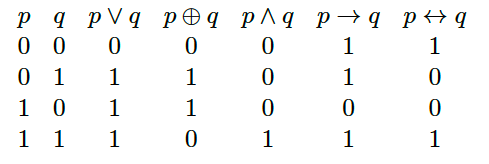
\includegraphics [width=3in]{Table-1-1-9-TableOfBitwiseLogic}
   \caption{Bitwise Logic}
   \label{table:bitwiselogic}
\end{table}

     \subsection{Evaluation of Compound Propositions}
Without parentheses compound logical statements can be ambiguous. But always explicitly including the parentheses leads to large numbers of them and makes the expressions harder to read. To avoid a large number of parentheses we adopt a convention of \textbf{operator precedence}. See Table \ref{table:precedenceOfLogicalOperators}.

\begin{table}[htbp]
   \centering
   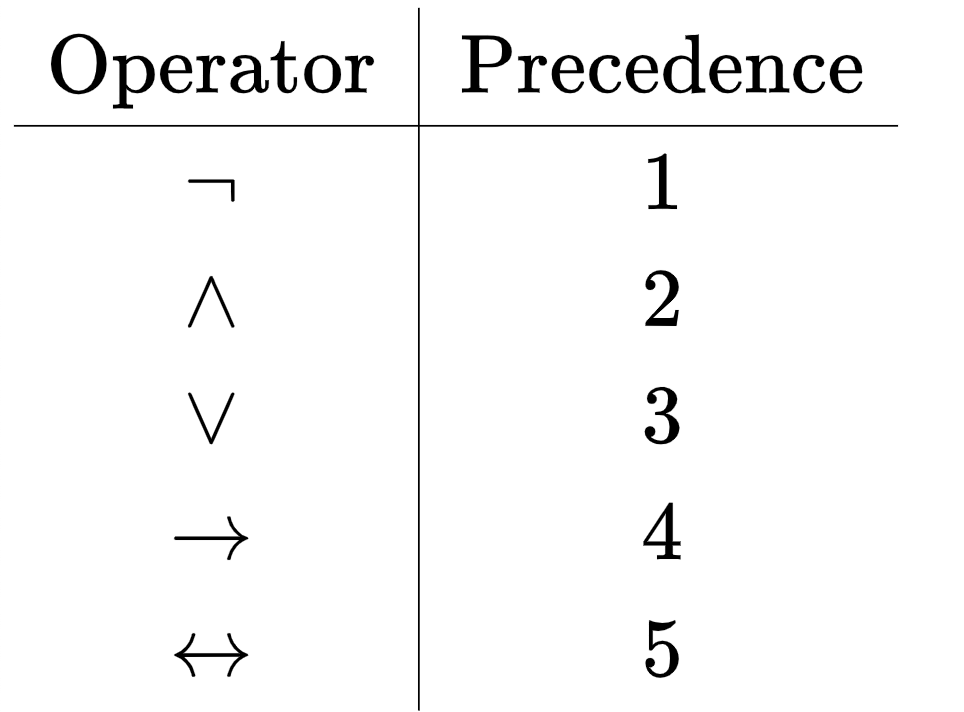
\includegraphics [width=1.5in]{PrecedenceOfLogicalOperators}
   \caption{Precedence of Logical Operators}
   \label{table:precedenceOfLogicalOperators}
\end{table}

      Truth Tables can be used to help derive the truth value of complex compound logic statements. Take the innermost binary operations required by the rules of precedence and create a column. Give the truth values for that small compound statement and then build up until you have the entire statement. 

    \subsection {Propositional Consistency}
consistent statements
    \subsection {Propositional Satisfiability}
\begin{definition}\index{satisfiability}
A compound proposition is \textbf{satisfiable} if there is an assignment of truth values to the variables in the compound proposition that makes the statement form true.
\end{definition}

\subsection{Paradox}
Some declarative statements defy a truth value. For example, ``This statement is false'' cannot be given a consistent truth value. If it is true, that the statement is false, then it must be true contradicting the assertion. Such a statement is called a \textbf{paradox}.


\begin {definition}\index{bit string}
A bit is a binary digit, typically a zero or a one. A bit string is a sequence of zero or more bits. The length of this string is the number of bits in the string. Given two bit strings of the same length we define bitwise operations:
\begin{enumerate}
\item bitwise OR, 
\item bitwise AND, 
\item bitwise XOR.
\end {enumerate}
\end{definition}





\subsection {Propositional Equivalences}

\begin {definition}[Tautology and Contradiction]\index{tautology}\index{contradiction}
A compound proposition that is always true , no matter what the truth value of the poisitons that occur in it, is called a \textit{tautology}. A compound proposition that is always false is called a \textit{contradiction}. A compound proposition that is neither a tautology nor a contradiction is called a \textit{contingency}.
\end {definition}

\begin {definition}[Logical Equivalence]\index{logical equivalence}
The compound proposition $p$ and $q$ are called \textit{logically equivalent} if $p \leftrightarrow q$ is  tautology. The notation $p \equiv q$ denotes that $p$ and $q$ are logically equivalent.
\end {definition}

Note: The symbol $\equiv$ is not a logical connective and $p \equiv q$ is not a compound proposition but a statement that $p \leftrightarrow q$ is a tautology. 

Two distinct propositions may evaluate to the same truth value for each combination of the atomic truth values. These two propositions are said to be logically equivalent or simply equivalent. This can be shown with a truth table and constitutes a valid proof of the equivalence. Logical equivalence leads to the principle that if two compound propositions always have the same truth values regardless of the values of the atomic propositions, then one can be substituted for the other where ever it appears.

  

  \begin{table}[htbp]
  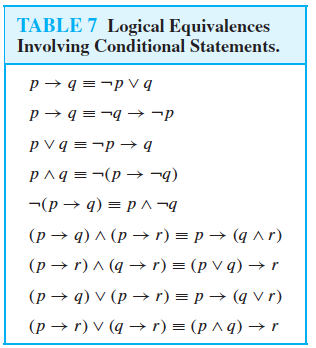
\includegraphics [width=3in]{Table-1-6-7-LogicalEquivalencesInvolvingConditionalStatements}
  \caption{Logical Equivalences Involving Conditional Statements}
  \label{table:logicalequivalencesinvolvingconditionalstatements}
  \end{table}
  
  \begin{table}[htbp]
  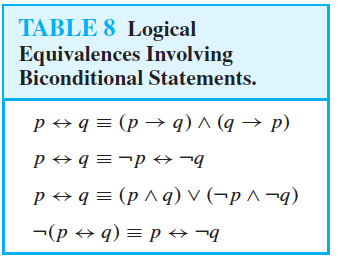
\includegraphics [width=3in]{Table-1-6-8-LogicalEquivalencesInvolvingBiconditonalStatements}
  \caption{Logical Equivalences Involving Bi-Conditional Statements}
  \label{table:LogicalEquivalenceInvolvingBiconditionalStatements}
  \end{table}

\begin{table}[htbp]
  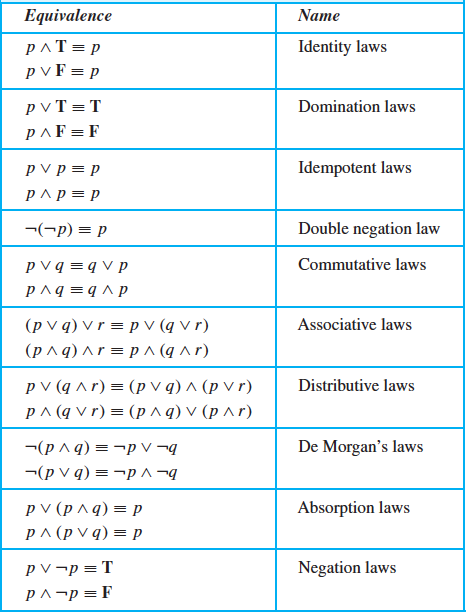
\includegraphics [width=3in]{Table-1-3-6-LogicalEquivalences}
  \caption{Logical Equivalences}
  \label{table:LogicalEquivalence}
  \end{table}




\section {Predicate Logic}
Predicate Logic. First order logic. There are other higher order logics. 
Propositional logic, zero order logic, cannot help with obviously true statements like, "Socrates is a man, all men are mortal, therefore Socrates is mortal". We need to introduce a way to prove such truths. This is called Predicate Logic or Predicate Calculus.

    \subsection {Predicates}
Some objects can have a property. A person may be tall or short. A number may be greater than 100. When we use variables to represent these objects we need a way to test them for the presence or absence of the quality we care about. We call these \textbf{propositional functions} and we call the quality being checked for \textbf{predicates}. 

For example, we may have a variable $x$ which is an integer. We can have a predicate which tests it to see if it is greater than 100. The predicate is "... is greater than 100" and we apply that to the variable $x$.

\begin{definition}[Predicate]\index{predicate}
A \textit{predicate} is a function which when applied to an object will evaluate to true when some property is present and false otherwise. We denote the predicate using a capital letter and write the expression using a functional notation. So the predicate $P$ when applied to the variable $x$ is written $P(x)$ and will take on the value of true or false when the value of $x$ has been fixed (bound).

Predicates are not limited to one argument but can have any number of arguments, called \textit{n-place predicates}. For example the predicate $S$ could be "...have the same color" and can accept pieces of fruit as objects. Then the expression $S(p,q,r,s,t)$ will be true if the color of each piece of fruit $p,q,r,s,t$ matches the others and false otherwise.

We often define a predicate using the notation, $P: x+1 > x$.
\end{definition}

\begin{notes}
More advanced texts may discard the parentheses around the arguments in a propositional function
\end{notes}

\begin{definition}{Value Assignment}
When we wish to indicate that a variable has been bound to a value, we use an assignment statement. We denote the assignment of the value c to the variable x with this notation: $x := c$. Some authors use $x\leftarrow c$ and many programming languages do this wil an equals sign, $x=c$. It helps to notice that there is an implied change of state from before and after the assignment. For example $t:=t+1$ must be understood to refer to the value of $t$ before the assignment while evaluating the expression and changing the value of $t$ with the assignment.
\end{definition}

We saw that the statement $x>2$ was not a proposition since $x$ is a variable. But once the variable is bound to a value it then has a truth value. We can denote this using this notation:
$[x:=1, (x>2)]$ and this will evaluate to false. We can also do this symbolically like this: $G:x>2$, [x:=3, G(x)] which will evaluate to true.

\subsection{Multi-place Predicates}
Some predicates take more than one variable. For example if we want to compare the color of two pieces of fruit, we can do it like so: $ASetOfFruit=\{apple, banana, papaya, grape,strawberry\}$, $SameColor(x,y):x is the same color as y$, $SameColor(apple,strawberry)=trie$, assuming the apple and the strawberry are both red.

Note how we specified that the variables are drawn from some set, which is called the \textbf{domain of discourse}. 

   \subsection {Quantifiers}\index{quantifier}\index{quantification}
Variables can be bound to values. But we often wish to assert a proposition over a range of values or to claim that there is an object with some property. This process of creating a proposition over some range of objects is called \textit{quantification}. The two fundamental quantifications are the universal and the existential.

        \subsubsection {Universal Quantification}\index{universe of discourse}\index{domain}
Many mathematical statements assert that a property is true for all values of a variable in a partiocular doman, called the \textbf{domain of discourse} (or \textbf{universe of discourse}, often just referred to s the \textbf{domain}. Such a statement is expressed using universal quantification. The universal quantification of $P(x)$ for a particular doman in the proposition that asserts that $P(x)$ is true for all values of $x$ in this domain. Note that the domain specifies the possible values of the variable $x$. The meaning of the universal quantification of $P(x)$ changes when we change the domain. The domain must always be specified when a universal quantifier is used; without it, the universal quantification of a statement is not defined.

\begin{definition}[Universal Quantification]\index{universal quantification}
The universal quantification of P(x) is the statement 
$$\text{"}P(x) \text{ for all values of }x \text{ in the domain."}$$
The notation $\forall x P(x)$ denotes the universal quantification of $P(x)$. Here $\forall$ is called the universal quantifier. We read $\forall x P(x)$ as "for all x P(x)" or "for every x P(x)". An element for which $P(x)$ is false is called a counterexample of $\forall x P(x)$.
\end{definition}

\begin{notes}
A domain of discourse must be provided when using universal instantiation. Generally an implicit assumption is made that all domains of discourse for quantifiers are nonempty. Note that if the domain is empty, then $\forall P(x)$ is true for any propositional function $P(X)$ because there are no elements $x$ in the domain for which $P(x)$ is false. 
\end{notes}

The changing the domain of discourse can change the evaluation of the predicate. For example if $P(x): x is purple$, if I wish to say that all eggplants are purple, I can say that when talking about eggplants, $\forall x P(x)$ is true but when talking about apples it is not true that $\forall x P(x)$. If you were to show me an eggplant that is not purple, you have given me a \textbf{counter example} and that will refute my assertion that all eggplants are purple. A single counter example is sufficient to refute a universal claim.

In the domain of natural numbers, what is the truth value of this assertion? $\forall n: n+1 > n$?

Consider $R:x^2 \ge x$ and the assertion $\forall x: R(x)$ in the domain of integers. Now consider it for the domain of reals.

It is sometimes helpful to think of a universal quantification as the conjunction of all elements in the domain when the domain is finite. For example if n is a natural number, $\forall n P(n) \equiv P(0) \land P(1) \land \dots \land P(n)$.

Translation challenge: All apples are sweet. $A(x): x is an apple$, $S(x): x is sweet$. Do you translate as $\forall x A(x) \land S(x)$ if the domain of discourse is the set of all fruits? No. It must be $\forall x A(x) \rightarrow S(x)$. Otherwise you are saying all fruits are sweet apples. 


        \subsection {Existential Quantifier}
Many mathematical statements assert that there is an element with a certain property. For example, for any integer $i$ there is another integer $j$ such that $i+j=0$. Such statements are expressed using existential quantification. With existential quantification, we for a proposition that is true if and only if $P(x)$ is true for at least one value of $x$ in the domain.

\begin{definition}\index{existential quantification}\index{existential quantifier}
The \textit{existential quantification} of $P(x)$ is the proposition
$$\text{"There exists an element }x \text{ in the domain such that } P(x) \text{ ."}$$
We use the notation $\exists x P(x)$ for the existential quantification of $P(x)$. Here $\exists$ is called the \textbf{existential quantifier}.
The domain must always be specified when a statement $\exists P(x)$ is used. The meaning of $\exists P(x)$ changes when the domain changes. without specifying the domain, the statement $\exists P(x)$ has no meaning. The existential quantifier $\exists P(x)$ is read as, "There is an $x$ such that $P(x)$, "There is at least one $x$ such that $P(x)$", or "For some $x P(x)$".
\end{definition}

\begin{notes}
Generally, an implicit assumption is made that all domains of discourse for quantifiers are nonempty. If the domain is empty, the $\exists P(x)$ is false whenever $P(X)$ is a propositional function because when the domain is empty, there can be no element in the domain for which $P(x)$ is true.\\

For finite domains, the existential quantifier can be thought of as a disjunction. For $n$ a natural number, $\exists n P(n)$ can be rewritten as $P(0) \lor P(1) \lor \dots \lor P(n)$.
\end{notes}

    \subsection {Other Quantifiers}
You will sometimes see other quantifiers but the only one which occurs often enough to get notice is the uniqueness quantifier:

\begin{definition}
The \textit{uniqueness quantification} of $P(x)$ is the proposition:
$$\text{"There exists exactly one element }x \text{ in the domain such that }P(x)\text{".}$$
We use the notation $\exists !$ for the uniqueness quantification.
\end{definition}

    \subsection {Quantifiers with Restricted Domains}
An abbreviated notation is sometimes used to specify some subset of the domain. For example $\forall x <0 (x^2 >0)$ in the domain of real numbers places the restrictive clause next to the quantifier.

The truth of an existential statement is proven by demonstrating one object that makes the predicate true. We call that object the \textit{witness}. To show that an existential statement is false we must show that no such object from the domain will make the predicate true. We must prove a negative. For example, if I assert that in the reals, $\exists x: x=x+1$, you cannot produce any such $x$. You could argue that the predicate is a contradiction since the equation $x=x+1$ is equivalent to $1=0$ which is clearly a contradiction. But many existential statements are not that easily proven false.

  

    
\begin{definition}[Binding Variables]\index{binding}
When a variable has been assigned a value, we say the value has been \textbf{bound} to the variable. Any variable that has not yet been bound to a value is said to be \textbf{free}. The \textbf{scope} of the binding is controlled by the use of parentheses or other marks. The value of a variable is also bound by the use of a quantifier and the variable is either within or outside the scope of that quantifier.
\end{definition}

Care must be taken  with quantified statements regarding the scope of the binding. When a variable is bound to a quantifier, all instances of that variable within the scope are bound. Any use of that variable outside the scope is unbound, or free. Within the scope of the binding a variable can be changed with no effect on the logic. For example $\forall a (Q(a) \land P(a))$, the quantifier binds $a$. We can rewrite this as $\forall b(Q(b) \land P(b))$. But if the expression is $\forall a Q(a) \land P(a)$, the first predicate is bound to the universal quantification but the second is not. The second use is \textit{unbound} or \textit{free}. Another example would be $\exists x:(x+y>x)$ the variable $x$ is bound but the variable $y$ is free.

\subsection {Precedence of Quantifiers}
We must update the precedence of the operators. Parentheses are still the  highest. But quantifiers come before propositional operators. The order of precedence places all propositional operators ahead of quantifiers. All quantifiers are equal precendence.


    \subsection {Logical Equivalences Involving Quantifiers}
\begin{definition}
Statements involving predicates and quantifier are \textit{logically equivalent} if and only if they have trhe same truth value no matter which predicates are substitued into these staeent and which domain of discourse is used for the variables in these propositionan functions. We use the notation $S \equiv T$ to indicate that two statements $S$ and $T$ involving predicates and quantifiers are logically equivalent.
\end{definition}

$\forall x (P(x) \land Q(x)) \equiv \forall x P(x) \land \forall x Q(x)$ regardless of the domain. 

    \subsection {Negating Quantified Expressions}
$\neg \forall x P(x) \equiv \exists x \neg P(x)$ is a logical equivalence.
$\neg \exists x P(x) \equiv \forall x \neg P(x)$ is a logical equivalence.
These are DeMorgan's laws again, this time for quantified statements. 
    
    \begin{table}[htbp]
  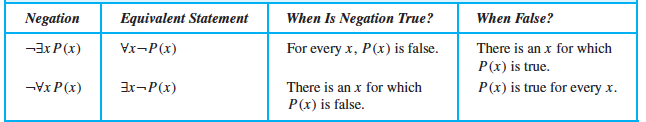
\includegraphics [width=3in]{DeMorgansForQuantifiedExpressions}
  \caption{DeMorgansForQuantifiedExpressions}
  \label{table:DeMorgansForQuantifiedExpressions}
  \end{table}
      
 


   \subsection {Nested Quantifiers and their Order}
   \begin{table}[htbp]
   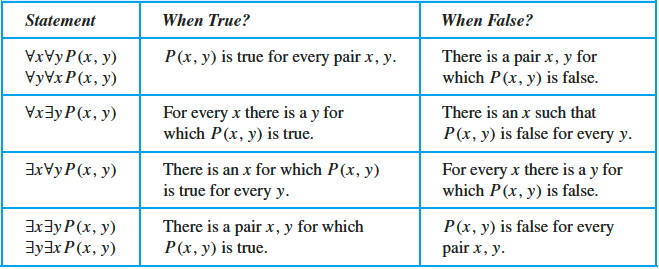
\includegraphics [width=3in]{Table-1-4-1-QuantificationOfTwoVariables}
  \caption{Quantification Of Two Variables}
  \label{table:QuantificationOfTwoVariables}
  \end{table}
  
It is important to note that the order of the quantifiers can make a difference. For example is this statement true or false for the domain of integers? $\forall x \exists y : (x+y=10)$. This is easily proven true with a bit of algebra. But what about $\exists y \forall x : (x+y=100)$. This is false since there is no such integer that will always give 10 when added to any other integer. 
 
  Universal quantifiers at the outermost level can be omitted, i.e., free variables are interpreted as universally quantified at the outermost level. Quantifiers can be applied to more than one variable at once (e.g., forall x,y). The infix equality sign (e.g., x = y) can be used as a shorthand for the equality predicate (e.g., equals(x,y)).
   \newpage 
    \subsection {Negating Nested Quantifiers}

Table-1-5-1-QuantificationsOfTwoVariables
\begin{table}[htbp]
  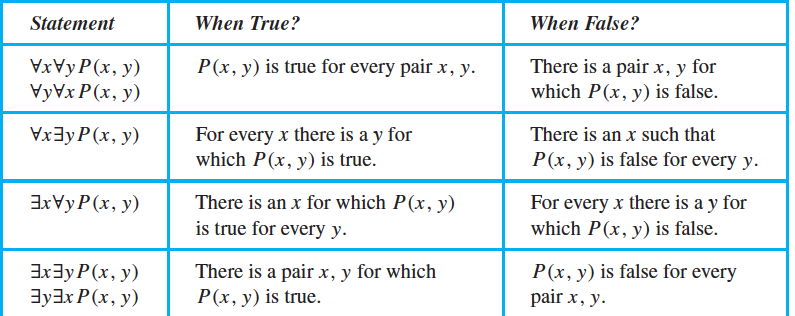
\includegraphics [width=3in]{Table-1-5-1-QuantificationsOfTwoVariables}
  \caption{Quant Of 2 Var}
  \label{table:QuantificationOfTwoVariables}
  \end{table}
  
\subsection{Thinking of Quantification as Loops}

THINKING OF QUANTIFICATION AS LOOPS In working with quantifications of more
than one variable, it is sometimes helpful to think in terms of nested loops. (Of course, if there
are infinitely many elements in the domain of some variable, we cannot actually loop through
all values. Nevertheless, this way of thinking is helpful in understanding nested quantifiers.) For
example, to see whether $\forall x \forall yP(x, y)$ is true, we loop through the values for $x$, and for each $x$
we loop through the values for $y$. If we find that $P(x, y)$ is true for all values for $x$ and $y$, we
have determined that $\forall x\forall yP(x, y)$ is true. If we ever hit a value $x$ for which we hit a value $y$
for which $P(x, y)$ is false, we have shown that $\forall x\forall yP(x, y)$ is false.
Similarly, to determine whether $\forall x\exists yP(x, y)$ is true, we loop through the values for $x$.
For each $x$ we loop through the values for $y$ until we find a $y$ for which $P(x, y)$ is true. If for
every $x$ we hit such a $y$, then $\forall x \exists yP(x, y)$ is true; if for some $x$ we never hit such a $y$, then
$\forall x\exists y P(x, y)$ is false.

To see whether $\exists x\forall yP(x, y)$ is true, we loop through the values for $x$ until we find an $x$ for
which $P(x, y)$ is always true when we loop through all values for $y$. Once we find such an $x$, we
knowthat $\exists x\forall yP(x, y)$ is true. If we never hit such an $x$, then we know that $\exists x\forall yP(x, y)$ is false.

Finally, to see whether $\exists x\exists yP(x, y)$ is true, we loop through the values for $x$, where for
each $x$ we loop through the values for $y$ until we hit an $x$ for which we hit a $y$ for which $P(x, y)$
is true. The statement $\exists x\exists yP(x, y)$ is false only if we never hit an $x$ for which we hit a $y$ such that $P(x, y)$ is true.

$S(x): x is a man$, $M(x): x is mortal$. Express ``all men are mortal, Socrates is a man, therefore Socrates is mortal''. $S(Socrates) \forall x S(x) \rightarrow M(x)$  (move to proofs where inference rule is discussed.)


   \subsection {Logic Programming}
An important type of programming language is designed to reason using the rules of predicate
logic. Prolog (from Programming in Logic), developed in the 1970s by computer scientists
working in the area of artificial intelligence, is an example of such a language. Prolog programs
include a set of declarations consisting of two types of statements, Prolog facts and Prolog
rules. Prolog facts define predicates by specifying the elements that satisfy these predicates.
Prolog rules are used to define new predicates using those already defined by Prolog facts.


	
         %%%%%%%%%%%%%%%%%   PROOFS   %%%%%%%%%%%%%%%%%%%%
\chapter{Introduction to Proofs}
For those who are already comfortable writing formal arguments and mathematical proofs, this chapter can be skipped. But many students approach the subject of proofs with trepidation and this chapter is included to connect the prior subject of formal logic and all the chapters that follow which develop their material with more formal presentations including proofs. 

To introduce proofs we will depend upon a few formal definitions that you learned in high school and prove some other properties using those definitions. 

\begin{definition}[Even and Odd Integers]
An even integer is one that is equal to twice some other integer. An odd integer is one that is equal to twice some other integer plus 1.
\end{definition}

But we must reiterate this text is not designed to teach but to provide a  support to the learning and later reference to the material within our scope. This is seen here in that other than a few examples needed to briefly illustrate some points, one will never learn to prove anything from this chapter. Instead it is a brief survey of basic terminology and cartoons of essential arguments to quickly remind the reader how to structure a proof of that type. We make some attempt in later chapters to give specific examples of the more interesting ways we reason about material using some of the techniques we present in its cartoon form in this chapter.

\section {Inference}
   \subsection {Valid Arguments in Propositional Logic}
\begin{definition}[Argument]
We define an \textit{argument} as some series of statements meant to convince the reader of the truth of some proposition we call the \textit{conclusion}.
\end{definition}

 
   \subsection {Rules of Inference for Propositional Logic}
We already saw how we can show the logical equivalence of two compound propositions using truth tables. However this becomes impractical as the number of atomic propositions grows. It also becomes difficult to follow the argument if this is the only way used to demonstrate the logical equivalence. In a high school geometry course you have already seen a different way that depends upon a series of statements and certain established rules of inference. We show how these are built from the logic.

One of the most basic is represented by this equivalence:
$$p \land (p \rightarrow q) \equiv q$$
This statement can be read as "Given that p is true with the the conditional statement if p is true that q must be true then it is logically equivalent to the value of q." When you construct the truth table you see this logical equivalence. This essential point of logic is called Modus Ponens, which is short for the Latin phrase "\textit{modus ponendo ponens}" which means "mode that affirms by affirming" and goes back to antiquity. It is also called the law of detachment. In more advanced material on logic this is considered beyond the logic presented up to now but we are not going to let that detail trouble us. It is the first of many argument forms that are used in argumentation. 

In antiquity logic came from rhetoric and the recognition that it was the rhetorical form that sometimes gave the truth or falsity of an argument and not the meaning of the propositions. That is why we jumped over natural language and the translations back and forth between symbolic logic and natural language. While an argument may sound persuasive, sometimes when reduced to its symbolic equivalent we can find a flaw in the argument.

The first thing you will notice is that this presentation of these rules of valid argumentation, or rules of inference, are not laid out like the compound propositions we saw before. In fact they are laid out in a way that mimics natural language by mimicing a sentence structure. For example I can state modus ponens in words as:\\
It is the case that whenever p is true that q is also true\\
It is the case that p is true\\
Therefore it is the case that q must be true. \\

It is customary to place a horizontal rule between the argument and the conclusion which is stated following the word, "therefore". Mathematicians have a symbol to mean therefore which is $\therefore$  . 

   \begin{table}[htbp]
   \centering
   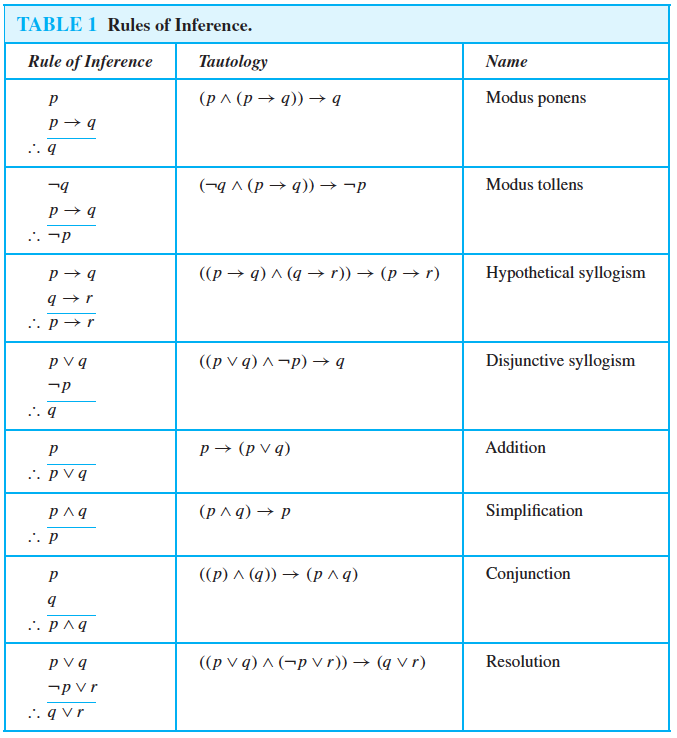
\includegraphics [width=5in] {Table-1-6-1-RulesOfInference}
   \caption{Common Rules of Inference}
   \label{table:rulesofinference}
   \end{table}

   \subsection {Using Rules of Inference to Build Arguments}
\begin{definition}[Argument Form]\index{argument form}
An argument in propositional logic is a sequence of propositions. All but the final proposition in the argument are called premises and the final proposition is called the conclusion. An argument is valid if the truth of all its premises implies that the conclusion is true.

An argument form in proposition logic is a sequence of compoutn propositions involving propositional variables. An arguent form is valid if no matter which particular propositions are substituted for the proposition variables in its premise, th econclusion is true if the premises are all true. (valid v sound??)
\end{definition}


If you look you will note that a great many properties in mathematics are stated as either conditional or bi-conditonal statements. "If $i$ is an even integer, then $i+1$ is an odd integer." If you want to mount an argument as to why this assertion must be true, you must demonstrate a series of equivalent statements that cannot be refuted until you reach the conclusion. In this case you will already have some definitions or other propositions that are not refuted, in this case the definiton of what it means to be even or odd. You must then offer the next assertion and be prepared to defend it. For example, "well if $i$ is an even integer then there is some other integer which I'll call $k$ such that $i=2k$ by the definition of what it means to be an even integer." Note that I have given both a new assertion, "there is some integer $k$ such that $i=2k$" and a justification, "\dots by the definition of what it means to be an even integer." In a classic two column presentation of the argument you would have one column which has the assert and another which has the justification for that assertion. You may have been taught this form in your high school geometry class. It helps you when you are first learning this style of formal argumentation since it forces you to support your argument (and makes grading so much easier!!!). Continuing our example, my next statement can be "$i+1=2k+1$, equals plus equals gives equals." We then can observe that "$2k+1$ is odd, by the definition of odd." Finally we conclude with "Therefore $i+1$ is an odd integer since it is equal to $2k+1$" and we have now completed the argument. A classic flourish in the presentation of such an argument is to put Q.E.D. which is the abbreviation for \textit{Quod Erat Demonstrandum}, a Latin phrase that means "that which was to be demonstrated." In textbooks this is often replace with a blackened or open square to signify that we reached the conclusion and the argument is over ($\blacksquare$ or $\square$). typographicallycalled a tombstone or Halmos.

Formal arguments like this are called proofs.

Note an important logical point about the prior argument. We claim it is application of the modus ponens inference. But where is the truth of the antecedent? Reconsider the implication, if $p$ then $q$. We already know that when the antecedent is false we evaluate the implication as true. That is to say in the last example that if it is the case that $i$ is NOT an even integer, that we make no claim about $i+1$. Once you ignore the two cases where the antecedent is false you only have two cases where it is true. For the conditional statement to be true we must argue that the case where the consequent is true is necessarily true and that the consequent must necessarily never be false. This allows us to accept the antecedent as true since we are only interested in conditionals with a true antecedent. If this does not make sense on the first reading, don't fret. But sooner or later it will occur to you that many conditional statements apply modus ponens without dealing with false antecedents. 

You will rarely see advanced mathematics texts with proofs set in a two column format. After your first introduction you are expected to be able to use a more natural prose method of presenting your formal arguments with no loss of precision in your logic. As you progress your need to justify each inference is reduced as you are writing for a more sophisticated reader who can make the most basic leaps of inference without aid. But like all non-fiction writing, you must know your audience. For a class like this one the expected reader needs to be a fellow student who may be slightly ahead or behind you. If you have any doubt that the rules of inference used are not obvious you need to put in remarks that do not interrupt the flow of the argument but support why the next assertion is valid.

From this point on in these notes where arguments are needed, you will see them presented in this fashion and we have tried to give you good examples of how to both structure your argument as well as lay them out on a page in a way that is consistent with tradition so as to make them easily understood by another mathematician. 

   \subsection {Resolution}\index{resolution}
Computer systems have come a long way in being able to do proofs. While it is not possible to do it in the general, they have been successful in many applicaitons. It should be noted that they make heavy use of one rule of interence called \textbf{resolution}. That rule of interence uses this tautology:
$$((p \lor q) \land (\neg p \lor r)) \rightarrow (q \lor r).$$
The consequent is called the resolvent. 

   \subsection {Fallacies}\index{fallacy}
Fallacies are important in rhetoric. Some mentioned in a rhetoric course are logical fallacies and not just rhetorical fallacies. It is important that you recognize the logical fallacies when they are presented. In discussing conditional statements we saw one which is mistaking the converse for the contrapositive. While $[(p \rightarrow q) \land p] \rightarrow q$ is a valid inference, it is NOT the case that $[(p \rightarrow q) \land q] \rightarrow p$. This second statement is the converse of the conditional assertion and we saw that the truth tables do not match. In rhetoric this is called the \textbf{fallacy of affirmig the conclusion}. 

In a very similar way, given the conditional statement $(p\rightarrow q)$ and $\neg p$ does NOT allow you to assert $q$. This is called the \textbf{fallcy of denying the hypothesis}. One of the strengths of symbolic logic over rhetoric is that seeing these fallacies is much easier in their symbolic form than when they are made in natural language. 

One other common fallacy is that of \textbf{affirming the disjunct}. Recall that for the logical \textit{or}, one or both of the terms may be true to give a true disjunction. But some people falsely argue that if one of the disjuncts is true the other must be false. This confuses the disjunction with the exclusive or.


   \subsection {Rules of Inference for Quantified Statements}
Up to now we have only looked at the rules of valid inference for propositional statements. Including predicate logic adds a few more. They are summarized in Table \ref{table:RulesOfInferenceForQuantifiedStatements}
   
  \begin{table}[htbp]
  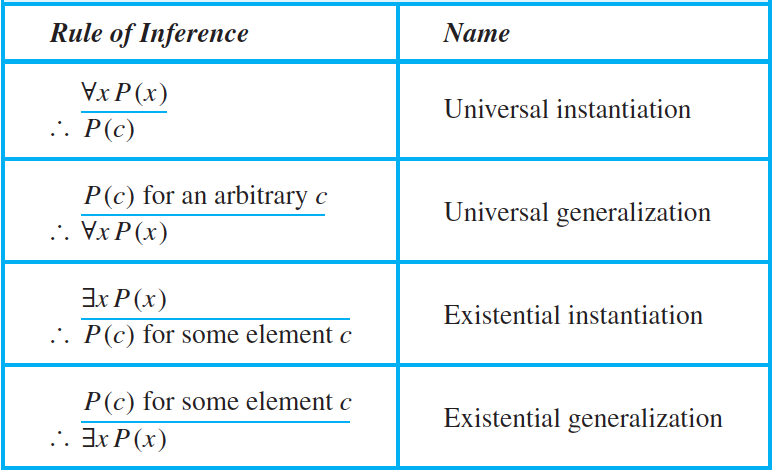
\includegraphics [width=3in]
  {Table-1-6-2-RulesOfInferenceForQuantifiedStatements}
  \caption{RulesOfInferenceForQuantifiedStatements}
  \label{table:RulesOfInferenceForQuantifiedStatements}
  \end{table}
  
   \subsection {Combining Rules of Inference for Propositions and Quantified Statements}
Here is one example of how the rules of inference for propositional logic can be applied with rules of inference for quantified statements as well. 

Given:
For all positive integers $n$, if $n$ is greater than 4, then $n^2$ is less than $2^n$,
Prove:
$$100^2 < 2^{100}$$


One inference rule that uses both propositional and predicate logic is \textbf{universal modus ponens}. This rule tells us that if $\forall x(P(x) \rightarrow Q(x))$ is true, and if $P(a)$ is true where $a$ is some specific member of the domain, then $Q(a)$ will also be true. Here is an example:

\begin{example}
Given that for all positive integers $n$, if $n$ is greater than 4, then $n^2$ is less than $2^n$, prove that $100^2 < 2^{100}$.
\begin{proof}
Let $P(n)$ denote "$n>4$" and let $Q(n)$ denote "$n^2$". The statement "For all positive integers $n$, if $n$ is greater than 4, then $n^2$ is less than $2^n$ can be represented by $\forall n(P(n) \rightarrow Q(n)$, where the domain consists of all positive integers. We start by assuming that $\forall n(P(n) \rightarrow Q(n)$ is true. Note that $P(100)$ is true because $100 > 4$. It follows by universal modus ponens that $Q(n)$ is true, namely that $100^2 < 2^{100}$. 
\end{proof}
 \end{example}
 
Note that this proof proceeded from its premises to its conclusion by applying one rule of inference or logic sequentially until the conclusion was affirmed. This is an example of a \textbf{Direct Proof}. Here is another example.

\begin{example}
Prove that if $n$ is an odd integer, then $n^2$ must be odd.
\begin{proof}
Note that this problem states $\forall n (P(n) \rightarrow Q(n))$, where "$P(n)$ is an odd integer" and "$Q(n)$ is $n^2$ is odd". The proof procedes by proving the implication. We begin the proof by assuming the antecedent of the implicaiton, that $P(n)$ is true and that $n$ is an odd integer. By the definition of an odd integer we have $\exists k : n=2k+1$, where $k$ is an integer. If we square both sides of the equation $n=2k+1$ we get $n^2=(2k+1)^2$ which gives us $4k^2+4k+1$. Factoring out 2 gives us $2(2k^2+2k) + 1$. We know that $k$ is an integer, that squaring an integer gives us an integer and that $2k$ will also be an integer and that adding an integer to an integer gives us an integer. Therefore we know that $(2k^2+2k)$ is an integer. This shows that the right side of the equation has the form twice some integer plus one which we know to satisfy the defintion of what it means to be odd. This proves that $n^2$ must be an integer satisfying the proof obligation to show that squaring an odd number must necessarily give us an odd integer. 
\end{proof}
\end{example}

There are times when the attempt to perform a direct proof  of an implication seems to lead to a dead end. When this happens it is sometimes easier to prove the contrapositive of the implication. This form of proof is called \textbf{Proof by Contraposition} as we demonstrate here:

\begin{example}
Prove that if $n$ is an integer and $3n+2$ is odd, then $n$ is odd.
\begin{proof}
We might proceed with the usual practice of assuming the antecedent and trying to derive the conclusion. This gives us that $3n+2$ is odd which means that $3n+2 = k+1$ where $k$ is some integer. We want to prove that $n$ is odd but there does not seem to be an easy way to proceed. We will try proving the contraposition instead. First we must state the contrapositive of the implication which we state as, if it is not the case that $n$ is odd, then it is not the case that $3n+2$ is odd.($\neg q\rightarrow \neg p$) We can use the fact that if something is not odd it must be even and restate the contraposition as, if $n$ is even, then $3n+2$ is even. If $n$ is even it can be restated as $2k$ where $k$ is some integer. Substituting we can restate the conclusion as $3(2k)+2$ or $6k+2$. We can factor out the 2 giving $2(3k+1)$ which fits the definition of an even number proving the consequent and concluding the proof.
\end{proof}
\end{example}

\begin{example}
Prove: If pigs can fly, then I sing better than Justin Bieber.
\begin{proof}
We are asked to prove another implication. In this case the antecedent of the implication is clearly false since we know that pigs cannot fly. Recall that an implication with a false antecedent is always true. A false premise can be used to "prove" anything.
\end{proof}
\end{example}

This is an example what is called a vacuuous proof. Here is a more interesting example.

\begin{example}
Prove that if $n = ab$, where $a$ and $b$ are positive integers, then $a \le \sqrt {n}$ or $b \le \sqrt{n}$
\begin{proof}
Because there is no obvious way of showing that $a \le \sqrt{n}$ or $b \le \sqrt{n}$
 directly from the equation $n = ab$, where $a$ and $b$ are positive integers, we attempt a proof by contraposition.
The first step in a proof by contraposition is to assume that the conclusion of the conditional statement “If $n = ab$, where $a$ and $b$ are positive integers, then $a \le \sqrt{n}$ or $b \le \sqrt{n}$'' is false.  That is, we assume that the statement $(a \le \sqrt{n}) \lor (b \le \sqrt{n})$ is false. Using the meaning of disjunction
together with De Morgan’s law, we see that this implies that both $(a \le \sqrt{n})$ and $(b \le \sqrt{n})$ are false.

This implies that $a > \sqrt{n}$ and $b > \sqrt{n}$. We can multiply these inequalities together (using the fact that if $0 < s < t$ and $0 < u < v$, then $su < tv$) to obtain $ab > \sqrt{n} \dots \sqrt{n} =n$. This shows that $ab \neq n$, which contradicts the statement $n = ab$. Because the negation of the conclusion of the conditional statement implies that the hypothesis is false, the original conditional statement is true. Our proof by contraposition succeeded; we have proved that if $n = ab$, where $a$ and $b$ are positive integers, then $a \le\sqrt{n}$ or $b \le \sqrt{n}$.
\end{proof}
\end{example}


The last section introduced a great deal of terminology and basic logical structure. But many feel that real mathematics, including logic, does not begin until one begins to reason about the material and attempt to determine new truths from the truths that are either accepted as true or which can be arrived at through reason. This chapter is a fast introduction to this mode of reasoning.

The chapter introduces the basic terminology of deductive reasoning and its presentation in the form of formal proofs. Various proof methods and strategies are summarized with classic examples. The remainder of the book will build upon this basis and demonstrate good proof style.

\section {Introduction to Proofs}
  \subsection {Why Write Proofs?}
Mathematics can be distinguished from other scientists by the kind of reasoning that we do. For reasons that this course explains, computer science is mostly a form of applied mathematics and therefore learning how to do mathematical proofs is a needed skill for a true computer scientist. Reasoning is often split into two types, inductive and deductive. Inductive reasoning is that which tries to generalize from a series of observations while deductive uses logic to conclude that an assertion must be true based on other statements that are already accepted as true. When someone gives a series of assertions that each build on what has come before and using accepted reasoning, we say they have proven their assertion and that the argument is a valid proof of the assertion. This has been a part of logic since at least Euclid's geometry and continues to be a cornerstone of undergraduate education. This chapter will be a poor substitute for a full semester course on the subject but should at least prepare the student for more formal work.

  \subsection{What Am I Allowed to Assume for this Proof?}
Given the emphasis on using accepted truths as premises, the student quickly finds themselves asking, what am I allowed to assume as either a premise or a rule of inference? The last chapter gave the most common ones from logic but often the student must use some high school algebra. The simple answer is that anything you could do in high school as valid algebra can be done in a proof for this course. More formally it must be something that can be justified by some argument to authority, which will be some previously published property. And of course it needs to be applied correctly. What cannot be done is to introduce a truth that in any way assumes the conclusion one is trying to make. We deal with that in this chapter when talking about fallacies.

Some students are uncomfortable with the handwaving of allowing that which was admitted in high school math. For reasons beyond the scope of this book it is not possible to put all of arithmetic onto a firm axiomatic basis. But to help the nervous here is a brief list of high school algebra: 
\begin{itemize}
  \item Closure Laws for Addition and Multiplication
  \item Associative Laws for Addition and Multiplication
  \item Commutative Laws for Addition and Multiplication
  \item Additive and Multiplicative Identity Laws
  \item Identity Elements Axiom
  \item Inverse Laws for Addition and Multiplication
  \item Distributive Laws
  \item Trichotomy Law
  \item Transitivity Law
  \item Additive Compatibility Law
  \item Multiplicative Compatibility Law
 \end{itemize}

For this text we take one more axiom that may not always be covered in a high school class but which we will need in the section on induction. That is called the \textit{completeness property}. This includes the definition of the upper bound and least upper bound. 

\begin{definition}[Completeness Property]\label{CompletenessProperty}
Every nonempty set of real numbers that is bounded above has a least upper bound.
\end{definition}


    informal proofs, theorem, propositions, facts, results, proof, axioms, postulates, lemma, corollary, conjecture
    \subsection {Understanding How Theorems Are Stated}
Often there is an \textbf{assertion} we want to make, some \textbf{proposition} which must either be true or false. Assertions often start as \textbf{conjectures}, propositions which we do not yet know are either true or false and which we would like to have a proof but do not yet have one. We often start with basic definitions which are essentially \textbf{axioms} that we accept as true without question. We must then construct a series of statements that each make new assertions by using the prior axioms and the \textbf{accepted rules of inference}. If we are successful, the final assertion is the proposition we wanted to prove which we call the \textbf{conclusion} of the argument. When we are presenting the assertion with the list of infered assertions that lead to the conclusion, we call this a \textbf{proof}. \textbf{Theorems} are nothing more than assertions we find helpful presented with their arguments as to why the assertion must be true. 

It is not uncommon that something accepted as an axiom is later found to be untrue, that is false. Or that a proof which depended upon a prior theorem which is found to contain a flaw. This leads to an important point about proofs, one can present a \textbf{valid} argument, one which uses only valid rules of inference, yet is found to depend upon one or more premises that are false. The argument is still said to be valid but the argument unsound. To be a \textbf{sound} argument one must have valid reasoning plus true premises. 



\section{Common Argument Forms}
\subsection {Direct Proofs}
In the chapter on Logic, there was a table of logical equivalences, Table \ref{table:LogicalEquivalenceInvolvingBiconditionalStatements}. The equivalence was demonstrated by showing that no matter the truth condition of the propositions, both expressions would evaluate to the same truth value. That is, the truth tables for both columns under the expressions matched on every row. This is a proof by truth table. However the number of rows will grow exponentially with the number of propositions so this kind of proof cannot be done by hand and often not even by machine for large numbers of propositions. 

This leads to the more common style of proof which is the series of statements grounded on the prior truths but making a new and equivalent statement. We stated the rule of inference known as Modus Ponens which says that given a true conditional statement and the fact that the antecedent of the conditional is known to be true, that the consequent of the conditional must be true. 

$$p \land (p \rightarrow q) \equiv q  \text{    (Modus Ponens)}$$
    
    
  \subsection {Direct Proofs}
\begin {theorem}
The sum of two even numbers is even
\begin{proof}[Two-Column Formal]
Let n,m be the two even numbers (premise given)\\
Then n=2*k and m=2*j where k and j are integers (def of even)\\
Then n+m=2*k + 2*j (basic law of arithmetic)\\
Then n+m=2*(k+j) (associative law of arithmetic)\\
Then n+m is even (def of even)   \\
\end{proof}
\end{theorem}

\begin{theorem}
The sum of two even numbers is even.
\begin{proof}[Prose Style]
Let $a$ and $b$ be the two even integers. We know by the definition of even that both can be expressed as twice two other integers $c$ and $d$ such that $a=2c$ and $b=2d$. Then the sum of $a+b$ can be expressed as $2c+2d$. After factoring out  the 2 we see that the sum fits the definition of even.
\end{proof}
\end {theorem}


    \subsection {Proof by Contraposition}\index{proof by contraposition}
    indirect proofs, vacuous and trivial proofs
    \subsection {Proofs by Contradiction}\index{proof by contradiction} 
    A proposition must be either true or false (rule of excluded middle). If it can be shown that a proposition cannot be false, then it must be true. To do this assume the opposite of what is to be proven and then show that it leads to a contradiction. Recall that a contradiction is false regardless of the truth values of the propositions. Once this is done you can assert that the contradiction is false and then conclude that the hypothesis must be true.
    \subsection {Exhaustive Proof and Proof by Cases}
    without loss of generality (WLOG)
    \subsection {Mistakes in Proofs}
    begging the question, circular reasoning


    
    

    \subsection {Looking for Counterexamples}
    \subsection {Proof Strategy in Action}
    \subsection {Additional Proof Methods}


\section{Proof Styles}
  \subsection{Proof by Truth Table}
If you can show that two statements always have the same truth value regardless of the truth value of the variables in the expression, you have demonstrated logical equivalence and one can always be substituted for the other where ever it appears. This can be done by creating a truth table with each expression at the top of a column and a row for every combination of truth values of the atomic propositions and show that the two columns have the same values on every row. But since the number of rows in a truth table grows exponentially with the number of atomic propositions, this method is only useful for small equivalences.
  \subsection{Two-Column Proofs}
High-school geometry teaches a two-column method. Some algebra classes use a similar approach to evaluating algebraic expressions. Most introductions to proofs begin with this form of proof presentation. Each line is a statement that is derived deductively from the lines above it. This is less tedious than a truth table proof and seems to correspond with how humans can follow detailed logic. In the most rigorous approach each line must list the inference explicitly in the right hand column to justify the statement just made. This has the advantage of making a student carefully understand how they are using logic to make the statements and easier for a grader to see that valid logic has always been applied. But the insistence on listing every rule applied makes the proof tedious for longer proofs as trivial points of logic clutter the work.
  \subsection{Prose Style Proofs}
Traditional mathematicians used a prose style of proof. The best of this technique applies all the rules of non-fiction writing. You make reasonable assumptions of what your reader will easily follow and which leaps of inference require some parenthetic remark to aid the reader. Good proof presentations in this form use natural language in a rigorous way yet will still suffer from an occassional slip  in inference. Yet by the end of the first introduction to proofs this is the way undergrads are expected to present their proofs. The vital point to recall is that any proof in this form could be reduced to a two-column proof if demanded. Experienced graders will look for large leaps and critically examine the inference to see if it is valid. If you feel it is correct but cannot justify it to yourself, take the time to break it into two or more steps that you can see the rule application.
  \subsection{Other Proof Styles}
There is an example of proof by combinatorial argument and a couple others in this and other texts. After the student becomes comfortable with these basics of formal argumentation we believe she will be well prepared to expand her ability to learn new techniques of mounting formal arguments.

Machine proofs are an area of research and many more rigorous proof styles have been described in the past 100 years. This is beyond the scope of an introductory proof class but we mention some of the notational forms used to prepare you for more advanced work. 

Note that many proofs are presented in this fashion and will use a notation called a turnstile $\vdash$:
    
\begin{comment}
\section {Methods of Proving Theorems}
This section describes the most basic form of proof style which is the direct proof and introduces the language with which we discuss proofs.
    \subsection {Direct Proofs}
In the chapter on Logic, there was a table of logical equivalences, Table \ref{table:LogicalEquivalenceInvolvingBiconditionalStatements}. The equivalence was demonstrated by showing that no matter the truth condition of the propositions, both expressions would evaluate to the same truth value. That is, the truth tables for both columns under the expressions matched on every row. This is a proof by truth table. However the number of rows will grow exponentially with the number of propositions so this kind of proof cannot be done by hand and often not even by machine for large numbers of propositions. 

This leads to the more common style of proof which is the series of statements grounded on the prior truths but making a new and equivalent statement. We stated the rule of inference known as Modus Ponens which says that given a true conditional statement and the fact that the antecedent of the conditional is known to be true, that the consequent of the conditional must be true. 

$$p \land (p \rightarrow q) \equiv q  \text{    (Modus Ponens)}$$
    
    \subsection {Proof by Contraposition}
    indirect proofs, vacuous and trivial proofs
    \subsection {Proofs by Contradiction}
    A proposition must be either true or false (rule of excluded middle). If it can be shown that a proposition cannot be false, then it must be true. To do this assume the opposite of what is to be proven and then show that it leads to a contradiction. Recall that a contradiction is false regardless of the truth values of the propositions. Once this is done you can assert that the contradiction is false and then conclude that the hypothesis must be true.

\subsection {Indirect Proof: Proof Using Contraposition}
Many proofs can be difficult to prove directly. But sometimes they are easier to prove using the contrapositive statement of the proof. This is just one common example of what is called an indirect proof. Recall that the contrapositive is the logical equivalent of any conditional statement. If you can prove the contrapositive, you have proven the conditional.

\subsection {Indirect Proof: Proof by Contradiction}
Not all proofs are given in the form of a conditional. Sometimes it is a direct assertion. Sometimes these statements can be proven using a technique called proof by contradiction or reducto absurdum. Do not confuse this with contrapositive. A contrapositive is the proof of a conditional statement while proof by contradiction is usually not. Proof by contradiction depends upon some basic truths of logic. A proposition must be either true or false, there is no other choice. This is called the law of the excluded middle. So if you can show that a statement MUST be false, then it must be true. How do you show that a statement must be false? If the statement can be restated as a contradiction, then it is false. 

The most famous example of a proof by contradiction is that the square root of 2 is irrational. This proof requires another definition from high school algebra that we state in a more casual fashion:

\begin{definition}[An Informal Definition of  Rational Number]
A rational number is one that can be expressed as the quotient of two integers.
\end{definition}

\begin{definition}[An Informal Definition of a Rational Number in Lowest Common Terms]
A rational number is in lowest terms when the numerator and denominator have no factors in common.
\end{definition}


\begin {theorem}
The square root of 2 is irrational.
\begin{proof}[Prove by contradiction: Assume the square root of 2 is rational.]
Since the square root of 2 is rational it can be expressed as the quotient of two integers. Let us call the two integers $a$ and $b$. If we divide out all common factors between $a$ and $b$, we are left with a new quotient $c/d$ of two integers with no common factor. This gives us $\sqrt{2}=c/d$ where $c/d$ is in lowest common terms. Squaring both sides give us $2=c^2/d^2$ which gives $2(d^2)=c^2$. The value $d^2$ must have an even number of the factor 2. Since we multiply this by 2 the value of $c^2$ has an odd number of the factor 2. However since $c^2$ is a square, it too must have an even number of the factor 2. This cannot be since an even number cannot also be a odd. We have derived a contradiction. In logic something cannot be both false and true and if we derive a contradiction we must reject the assumption we made as false and affirm its opposite, in this case that the square root of two must be irrational.
\end{proof}
\end {theorem}



Using the rule of substitution, we can use the rules of equivalence to give us an algebra of propositional logic. Any equivalence rule gives us an alternative way to write the expression that preserves the truth value. Note that in a truth table any two propositions will have identical columns in a truth table. In general while a truth table can be used to show equivalence, once you have more than 4 atomic propositions proving that two expressions are equivalent is more easily done with algebra than with truth tables.

argument: a set of propositions (premises) that is asserted to result in another proposition (conclusion). We formalize this to "prove" things. We say that an argument is valid when the conclusion is true whenever all the premises are true. An argument which is not valid is said to be a fallacy. A valid argument where all the premises are true is said to be sound.

We can write this in two ways:
Let P1, P2, P3, etc be a set of axioms and let Q be the conclusion

sentential, and this is equivalent to the logical statement
$P1 ^ P2 ^ P3^ ... |- Q$
and sometimes it is written as P1, P2, P3, ... |- Q where the conjunction is understood.

or 

P1
P2
P3
(underline)
therefore Q
QED

QED is short for Quod Erat Demonstrandum which means "that which was to be demonstrated. In typeset material the QED is often replaced with a black square.

There are a set of arguments that are used so often they have been given names. For example 

p, p -> q, |- q 

is known as Modes Ponens. These common arguments are summarized in Table 1.2: Rules of Inference. Note you are always free to create a new rule of equivalence.

Modus Ponens
Modus Tolens

Proof
A proof is an argument such that it accepts a certain number of propositions (axioms) which are taken to be true and using valid rules of inference and rules of equivalence results in stating the conclusion. To be a valid proof each line in the proof must be either an axiom or it must be supported by some rule of equivalence or inference. All students begin writing proofs by exhaustively showing the rules they used in a line-by-line format. But as you become more sophisticated you are allowed to skip steps that you assume the reader can follow. However if challenged you must always be prepared to give the step-by-step explanation of the reasoning.


What Can You Assume in Writing a Proof?
Students new to the formalism of mathematics can become confused as to what logical steps do not need support. In general for this class you can assume that everything you learned in secondary school can be used without support. Within a week (for the summer session) you can begin to drop the simplest logical steps and combine them. If there is doubt that the reader (your grader) will be able to see the steps you took to get to your conclusion, it is always ok to over simplify. And if you are unsure of the steps, it is always helpful to over simplify since the grader can point to the specific step you took which was invalid.

other ways are called indirect proofs
    \subsection {Proof by Contraposition}
        \subsubsection {Vacuous and Trivial Proofs}
 
\subsection {Proof Methods and Strategy}
  \subsection {Exhaustive Proof and Proof by Cases}
  \subsection {Existence Proofs}
  \subsection {Uniqueness Proofs}
    \subsection {Mistakes in Proofs}
    begging the question, circular reasoning
    \subsection {Just a Beginning}
  
\section {Proof Methods and Strategy}
    \subsection {Exhaustive Proof and Proof by Cases}
    without loss of generality (WLOG)
    
    
    \subsection {Proof Strategies}
    \subsection {Looking for Counterexamples}
    \subsection {Proof Strategy in Action}
    \subsection {Additional Proof Methods}
\end{comment}

\subsection {Proof Strategies}
  \subsection {Looking for Counterexamples}
Any assertion using a universal quantification can be refuted by citing a single counterexample.


\section{Formal Methods}
An important application of proof techniques is found in the study of what is called formal methods which includes proofs of program correctness


  \subsection {Program Verification}A program is said to be correcrt if it produces the correct output for every possible input. A proof of correctness for a program consists of two parts. The first part shows that the correct answer is obtained if the program terminates. This part is said to establish the partial correctness of the program. The second part proves that the program always terminates. When working with proofs of program correctness we use two propositions. The first, called the pre-conditions, gives a proposition that all input values must satisfy. In addition the second proposition is called the post-condition and if the program has correctly computed the value it will evaluate to true. The pre- and post-conditions are sometimes called the initial and final assertions.

\begin{definition}
A program, or program segment, $S$ is said to be partially correct with respect to the initial assertion $p$ and the final assertion $q$ if whenever $p$ is true for the input values of $S$ and $S$ terminates, then $q$ is true for the ouptut values of $S$. The notation $p[S]q$ indicates that the program, or program segment, $S$ is partially correct with respect to the initial assertion $p$ and the final assertion $q$. The notation $p[S]q$ is known as a \textit{Hoare triple}.
\end{definition}

 {Rules of Inference}
composition rule
   {Conditional Statements}
  {Loop Invariants}
        
\newpage





	


  



                          %%% SETS %%%
\chapter {Sets}

\section {Set Definition}
%This is only an introduction to set theory as originally presented by Georg Cantor, now known as naive set theory to set it apart from later work which attempts to put it onto an axiomatic basis. 

\begin {definition}
A \textit{set} is an unordered but well defined collection of objects which are called the \textit{elements/members} of the set.  The objects in a set are called the \textit{elements} or \textit{members}, of the set. A set is said to \textit{contain} its elements. We write $a \in A$ and say, ``a is an element of the set A'' to mean that $A$ contains $a$ and $a \notin A$ to mean that the element $a$ is not contained by the set $A$.
\end {definition}

\begin{notes}
   Sets are unordered. \{a, b\} is the same as \{b, a\}. The number of times an object is enumerated makes no difference, it is still one element.
\end{notes}


  \section{Set Specification}
    \subsection {Set Enumeration}
  The easiest way to describe small sets is to enumerate (list) the elements. This is done by writing the elements between braces with a comma between them. For example let $V$ be the set of English vowels. We can write $V=\{a,e,i,o,u\}$ to define the set $V$. If we want to talk about the positive odd integers less than 10 as the set $O$, we can define it as the set $\{1,3,5,7,9\}$. 
The set $M=\{1, "1", \text{my dog Rover}, \text{red-head}\}$ can be a set. The notation $a_1,a_2,a_3 \in A$ is the same as $a_1 \in A, a_2 \in A, a_3 \in A$. We can start a pattern and use the ellipses symbol to indicate that the reader should infer the pattern. R=\{3,6,9,12,15, \dots\}. $\{0,1,2,3, \dots ,100\}$ The enumeration can be a description of the elements. \{addresses on Pine Street\} defines a set of addresses that are on Pine Street. $O=\{ \text{positive odd integers less than 10} \}$. 


     \subsection {Set Builder Notation}
Set comprehension, set intension. Three parts, a variable, a colon or vertical bar and a logical predicate.  


$\{a | \text{  a is a positive integer }\} $

or 

$E: \text{is even}$, 
$A= \{a | E(a)\}$\\
We read this as 
set A is defined as the set of all $a$ such that $a$ is even. The vertical bar is read "such that". To the left are the variables that represent the set members and to the right is the condition that all members must satisfy.

Example: $A = \{x | \lnot E(x),x<10\}  $

\begin{notes}
Predicates separated by commas are implied conjunction.
\end{notes}
  
Sometimes we restrict the domain of a quantified statement explicitly by making use of a particular notation. For example, $\forall x \in S (P(x))$       %∀x∈S(P(x)) 
denotes the universal quantification of $P(x)$ over all elements in the set $S$. In other words, $\forall x \in S (P(x))$  is shorthand for $\forall x (x \in S(P(x)) \rightarrow P(x))$    
%∀x∈S(P(x)) is shorthand for ∀x(x ∈ S → P(x)).
Similarly, $\exists x \in S(P(x))$ denotes the existential quantification of $P(x)$ over all elements in $S$. That is, $\exists x \in S(P(x))$ is shorthand for $\exists x (x \in S \land P(x))$.
%Similarly, ∃x∈S(P(x)) denotes the existential quantification of P(x) over all elements in S.
%That is, ∃x∈S(P(x)) is shorthand for ∃x(x ∈ S ∧ P(x)).


\section {Common sets and their Notation in Mathematics and Computer Science}
 $\mathbb{N}=\{1,2,3, \dots \} \text {the set of \textbf{natural numbers} } $ \\
 $\mathbb{Z}=\{\dots -3,-2,-1,0,1,2,3, \dots\}  \text{The set of } \textbf{integers}$ \\
 $\mathbb{Q}=\{\dfrac{p}{q} | p \in \mathbb{Z}, q \in \mathbb{Z}, q \neq 0 \} \text{The set of \textbf{rational numbers}}$ \\
 $\mathbb{R}=\{ \text{the set of }\textbf{real numbers}   \} $ \\
 $\mathbb{C}=\{ \text{the set of }\textbf{complex numbers} \} $ \\
 $\mathbb{B}=\{0,1\} \text{ the set of \textbf{a set of binary symbols} } $ \\
 





\begin {notes}
 We can restrict the universe from which the objects are drawn to the right of the "$|$" like so: \\
 $O=\{\mathbb{Z}^+ | x \text{ is odd and } x<10 \}$  \\
This is read as "The set O is equal to the set of all x drawn from the set of positive integers such that x is less than 10."
The superscript indicates that only the positive members of the domain are to be considered.
Zero may or may not be considered a natural number depending upon the author. For this course we accept zero as a natural number and use the notation $\mathbb{Z}^+$ for the set of positive integers. The special font used for these special sets is called Blackboard Bold. Z is used for integers because the German word for numbers is Zahlen.
\end{notes}

  A set is an object. Therefore we can have a set which contains other sets:
  $$ \text{Basic data types} = \{\mathbb{B}, \mathbb{N}, \mathbb{Z}, \mathbb{R} \}$$
This fact leads to interesting paradoxes which mark the difference between what is known as Naive Set Theory and more advanced forms.

\begin{notes}
Sets and data types in programming languages are related.\\
There is a shortcut used sometimes to assert a universal truth for a set. For example $\forall x \in S(P(x))$ which asserts that all elements of the set $S$ have property $P$. It can also be stated as $\forall x(x \in S \rightarrow P(X))$
\end{notes}

\section {Truth Sets}
\begin {definition}[Truth Sets]\index{truth set}
Given a predicate $P$, and a domain $D$, we define the \textbf{truth set} of $P$ to be the set of elements $x$ in $D$ for which $P(x)$ is true. The truth set of $P(x)$ is denoted by$ \{ x \in D | P(x) \} $.
\end {definition}

  
\section {Set Equality}
\begin {definition}[Set Equality]\index{set equality}
Two sets are \textit{equal} if and only if they have the same elements. That is, if $A$ and $B$ are sets, then $A$ and $B$ are equal if and only if $\forall x(x \in A \leftrightarrow x \in B)$. We write $A=B$ if $A$ and $B$ are equal sets.
\end {definition}
\begin{notes}
Some authors will use $\subset$ specifically to designate a proper subset and use $\subseteq$ for subsets that could be equal. We only use $\subset$ in these notes to indicate either a proper subset or an equal set.
\end{notes}
  
\begin{definition}[Empty Set]\index{empty set}
A set that contains no elements is called \textit{null set} or \textit{empty set}and is denoted by $\emptyset$. The empty set can also be denoted by $\{ \}$
\end{definition}

\section{Subsets}
  If a set is composed of elements of another set, we call the new set a \textbf{subset}. The subset may have all the same elements as the first set. If it has fewer elements, we may call it a \textbf{proper sub-set}.
  
\begin {definition}[Subset]\index{subset}
A set $A$ is said to be a \textit{subset} of $B$ if and only if every element of $A$ is also an element of $B$.  We write $A \subset B$ to indicate that $A$ is a subset of $B$ and $A \not\subset B$ to indicate that $A$ is not a subset of $B$. $\forall x(x \in A \rightarrow x \in B)$ is true whenever $A$ is a subset of $B$.
\end {definition} 

\begin {theorem}
$A=B$  if and only if $A \subset B$ and $B \subset A$
\end {theorem}

 \subsection{Intervals of Reals}  
  We frequently talk about subsets of the reals or integers  as intervals. There are conflicting notations.

\begin{align*}
 \big( a,b\big) = &\big] a,b\big[ &= \{ x \in \mathbb{R}   |   a < x < b       \}, \\
 \big[a ,b\big) = &\big[ a,b\big[ &=  \{ x \in \mathbb{R}  | a \le x<b      \}, \\
 \big(a ,b\big] = &\big] a,b\big] &=  \{ x \in \mathbb{R}  | a < x \le b       \}, \\
 \big[ a,b\big] = &\big[ a,b\big]  &=  \{ x \in \mathbb{R} | a \le x \le  b  \}.
\end{align*}
For intervals that extend to infinity toward the negative or positive infinity, we substitute $-\infty$ for $a$ or $+\infty$ for $b$.

 \subsection{Integer Intervals}
 The notation $\big[ a \ldots b\big] $ when $a$ and $b$ are integers, or $\big\{a\ldots b\big\}$ , or just $a\ldots b$ is sometimes used to indicate the interval of all integers between $a$ and $b$, including both. This notation is used in some programming languages; in Pascal, for example, it is used to formally define a subrange type, most frequently used to specify lower and upper bounds of valid indices of an array.
 
 An integer interval that has a finite lower or upper endpoint always includes that endpoint. Therefore, the exclusion of endpoints can be explicitly denoted by writing $a\ldots b-1$,$a+1\ldots b$, or $a+1\dots b-1$. Alternate-bracket notations like $[a\ldots b)$ or $[a\ldots b[$ are rarely used for integer intervals.

\begin{definition}
We denote the set $\{0,1,\dots m-1\}$ with the notation $\mathbb{Z}_m$.
\end{definition}

  
\section {Universal and Empty Sets}
\begin {definition}[Universal and Empty Sets]\index{universal set} \index{empty set}
The \textit{universal set} or universe is a set that represents some domain of discourse. There is no symbol that everyone accepts as the symbol for the universal set. We adopt $\mathbb{U}$ to designate the universal set.
The set which contains no elements is the \textit{null} or \textit{empty set} and is disignated by $\emptyset$. 
\end {definition}

\begin{notes}
Never confuse $\emptyset$ with \{$\emptyset$\}. The first is a set which contains no elements. The second is a set which contains one element and that element is a set which contains no elements. Think of file folders on a disk as sets and files as elements.
\end{notes}

 \begin {theorem}
For any set S, the following are true:\\
$\emptyset \subset S$ , \\
$S \subset \mathbb{U}$, \\
$\emptyset \text{ is unique}$\\
For any set $S, \emptyset \subset S \subset \mathbb{U}$
\end {theorem}


\section {Set Operators}

\begin {definition} [Set Union]\index{set union}
Let $A$ and $B$ be sets. The \textbf{union} of the sets $A$ and $B$, denoted by $A \cup B$, is the set that contains those elements that are either in $A$ or in $B$, or in both. $A \cup B=\{x:x \in A \lor x \in B\}$
\end {definition}

\begin{figure}[htbp]
   \centering
   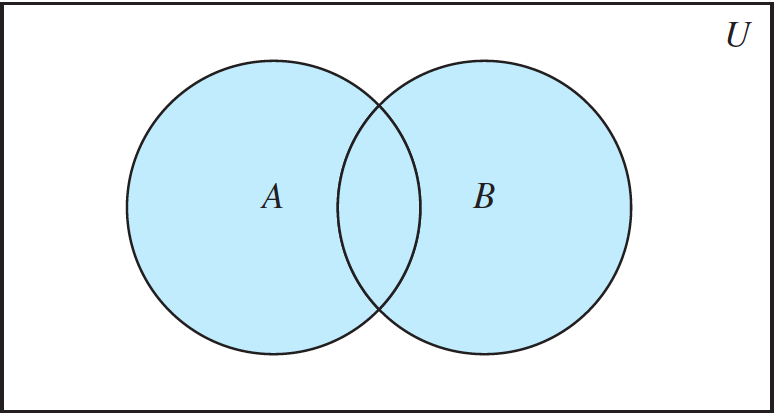
\includegraphics [width=3in]{Figure-2-2-1-VennDiagramOfAUnionB}
   \caption{Venn Diagram Of A Union B}
   \label{figure:Venn Diagram Of A Union B}
\end{figure}
   
\begin {definition}[Set Intersection]\index{set intersection}
Let $A$ and $B$ be sets. The \textbf{intersection} of the sets $A$ and $B$, denoted by $A \cap B$, is the set containing those elements in both $A$ and $B$.
$A \cap B = \{x:x \in A  \land x \in B\}$
\end {definition}

\begin{figure}[htbp]
   \centering
   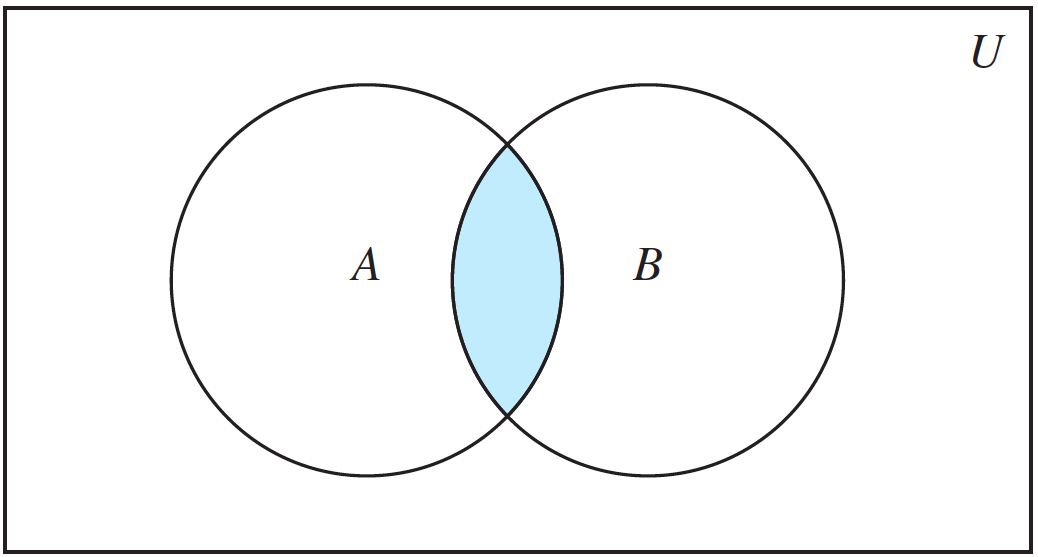
\includegraphics [width=3in]{Figure-2-2-2-VennDiagramOfTheIntersectionOfAandB}
   \caption{Venn Diagram Of The Intersection Of A and B}
   \label{figure:Venn Diagram Of The Intersection Of A and B}
\end{figure}

\begin {definition}[Disjoint Sets]\index{disjoint sets}
Two sets are disjoint if and only if $A \cup B = \emptyset$
\end {definition}

\begin {definition}[Set Difference]\index{set difference}
Let $A$ and $B$ be sets. The \textit{difference} of $A$ and $B$ denoted by $A - B$ and sometimes by $A \setminus B$ according to the ISO 31-11 standard, is the set containing those elements that are in $A$ but not in $B$. The difference of $A$ and $B$ is also called the \textit{complement of B with respect to A}.
$A - B = \{x | x \in A \land x \notin B\}$.
\end {definition}

 It is sometimes written $B - A$, but this notation is ambiguous, as in some contexts it can be interpreted as the set of all elements $b - a$, where b is taken from B and a from A.

\begin{definition}[Symmetric Difference]\index{symmetric difference}
The symmetric difference of $A$ and $B$, denoted by $A \oplus B$, is
the set containing those elements in either $A$ or $B$, but not in
both $A$ and $B$.
\end{definition}

\begin {definition} [Set Complement]\index{Set Complement}
$A^C$ or $ \bar{A} $ is called a set complement. It is all elements of the universal set which are not contained in the set $A$.
\end {definition}

\section {Identities of Set Algebra}
Set operators give identities that can be proven. The following are a list of the most basic identifies and the names they are given. Any of these can be proven using the formal definition of the operator and the rules of equivalence and inference from logic.


   \begin{table}[htbp]
   \centering
   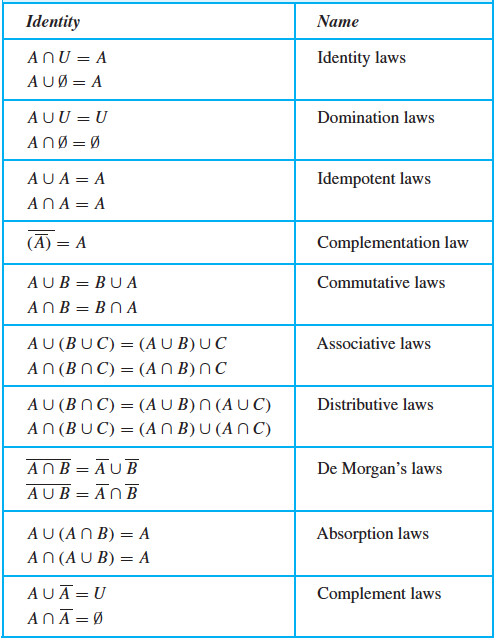
\includegraphics [scale=0.5]{Table-2-2-1-SetIdentities}
   \caption{Set Identities}
   \label{table:Set Identities}
   \end{table}


\begin{notes}
Note the similarity to Identities of Logic 
\end{notes}

\section {Venn Diagrams}
    Diagrams that represent sets as ovals within a square box with or without labeled elements are called Venn diagrams. The outer box represents the universe of discourse, $U$, for the sets.   In a Venn diagram, the universal set is th einterior of a rectangle. If $A \subset B$, then the area of $A$ will be contained within the area of $B$.
If $A$ and $B$ are disjoint, then the area of $A$ will overlap art of the area of $B$.

   \begin{table}[htbp]
   \centering
   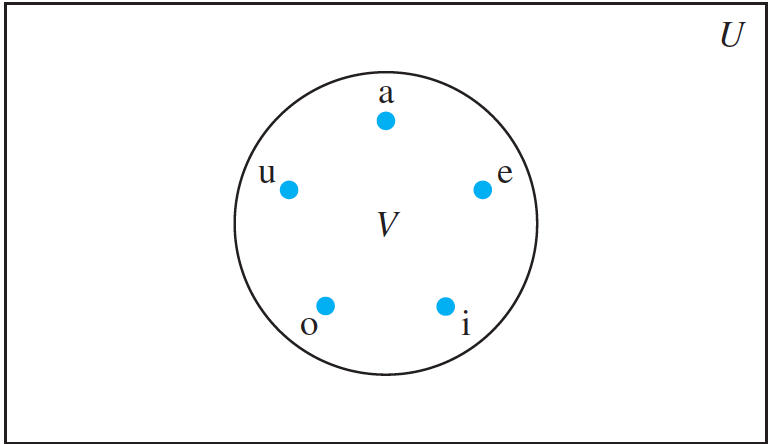
\includegraphics [width=2in]{Figure-2-1-1-VennDiagramOfVowels}
   \caption{VennDiagramOfVowels}
   \label{figure:VennDiagramOfVowels}
   \end{table}



    \begin{definition}[Set Cross Product or Cartesian Cross Product]\index{set cross product}
The ordered n-tuple $(a_1, a_2, . . . , a_n)$ is the ordered collection that has $a_1$ as its first element, $a_2$ as its second element, . . . , and $a_n$ as its $n$th element.
Two tuples are considered equal if and only if all corresponding elements of the two tuples match.

$$A \times B = \{(a,b)\mid a \in A \land b \in B\}$$
    \end{definition}

    \begin{definition}
    Let $A$ and $B$ be sets. The Cartesian product of $A$ and $B$, denoted by $A \times B$, is the set of all
ordered pairs $(a, b)$, where $a \in A$ and $b \in B$. Hence,
$A \times B = \{(a, b) \vert a \in  A \land b \in B\}$.
    \end{definition}
    
$A \times B$
\begin{notes}
The elements of a tuple are ordered. $(a,b)$ is not the same as $(b, a)$.\\
Cross products of sets to themselves can be represented with superscripts. $A^2=A \times A$.\\
The cross product is a SET of TUPLES.
\end{notes}

    \begin {definition}
    The Cartesian product of the sets $A_1,A_2, . . . , A_n$, denoted by $A_1 \times A_2 \times \dots \times A_n$, is the
set of ordered n-tuples $(a_1, a_2, . . . , a_n)$, where $a_i$ belongs to $A_i$ for $i$ = 1, 2, . . . , n. In other
words,
$A_1 \times A_2 \times \dots \times A_n = \{(a_1, a_2, . . . , a_n) | a_i \in A_i$ for $i = 1, 2, . . . , n\}$.
    \end {definition}

\section {Set Cardinality}
\begin {definition}[Set Cardinality]\index{set cardinality}
The size of the set is the number of elements in the set for sets with a finite number of elements. We will defer infinite sets until later. This is called the set \textit{cardinality}. It is denoted by $\mathbf{card}(S)$ or $|S|$.
\end{definition}

\begin{definition}[Powerset]\index {powerset}
A special set called the power set is that set which includes every possible and unique subset of some set $S$. 
Note: the easiest way to enumerate the subset is by the number of elements in the set. List all the subsets with zero members (only one, the null set). Then all the subsets of size 1, 2, etc. 
\end{definition}
\begin {theorem}
If the size of set $S$ is $m$, there are $2^m$ posible subsets.
\end{theorem}

Special symbol  $\mathcal{P} (A)$ designates the power set of set A.

\begin{notes}
the powerset IS A SET of SETS
\end{notes}


\section {Indexed Sets/Indexed Classes of Sets and Generalized Set Operations }
%NOTE: the requires functions!!
Let $I$ be any nonempty set (not necessarily a numeric set), and let $S$ be a collection of sets. An indexing function from $I$ to $S$ is a function $f:I \rightarrow S$. For an $i \in I$, we denote the image $f(i)$ by $A_i$. Thus we can say:

$\{A_i : i \in I\} or \{A_i\} \in I$, or simply $\{A_i\}$

The set $I$ is called the \textbf{indexing set} and the elements of $I$ the \textbf{indices}. 

When many sets are joined or intersected, we introduce an indexed notation:


$\cup _{ i=1} ^ n a _{i}$

$\cap_{ i=1} ^ n a _{i}$


(give Venn diagram)

Representations of sets, set membership tables.


\begin{definition}[Fundamental Product of Sets]\index {Fundamental Products of Sets}
Consider a set of sets $A_1$, $A_2$, etc that are all unique. 
Now let $A_i^*$ mean either $A_i$ or  $A_i^c$, that the notation $A_i^*$ either means $A_i$ or it means $A_i^c$.
The fundamental product of the set $S$ is that is the union of all sets denoted by $A^*$
\end{definition}
\begin{notes}
there are m sets, $2^n$ such fundamental products (why?)
any two fundamental products are disjoint
the union of all the fundamental products is the universal
\end{notes}



\begin{definition}[Partitions of a Set]\index{partitions of a set}
A \textbf{partition} of a set $S$ is a collection of disjoint nonempty subsets of $S$ that have $S$ as their union. Equivalently we can say the collection of subsets $A_i$, $i \in I$ where $I$ is an index set) forms a partition if and only if
$$A_i \neq \emptyset \text{  for  } i \in I$$
$$A_i \cup A_j =  \emptyset \text{  when  } i \neq j$$
$$\bigcup_{i \in I} A_i = S$$
\end{definition}

\section {Multisets and Bags}\index{multiset} \index{bag}
A \textit{multiset} is a set that does not require each object to be unique. It can be represented by a set of pairs with the first element of the pair representing the object and the second representing the \textit{multiplicity} of that object in the multiset. These are sometimes called \textit{bags}

Sometimes the number of times that an element occurs in an unordered collection matters. Multisets are unordered collections of elements where an element can occur as a member more than once. The notation $\{m_1 \cdot a_1, m_2 \cdot a_2, \dots ,m_r \cdot a_r\}$ denotes the multiset with element $a_1$ occurring $m_1$ times, element $a_2$ occurring $m_2$ times, and so on. The numbers $m_i, i=1,2,3, \dots r$ are called the multiplicies of the elements $a_i, i=1,2,3, \dots ,r$.

%Sometimes the number of times that an element occurs in an unordered collection matters. Multisets are unordered collections of elements where an element can occur as a member more than once. The notation {m1 · a1, m2 · a2, . . . , mr · ar } denotes the multiset with element a1 occurring m1 times, element a2 occurring m2 times, and so on. The numbers mi , i = 1, 2, . . . , r are called the multiplicities of the elements ai , i = 1, 2, . . . , r.

\section{Strings}\index{string}
We noted that a set cross product may not have a numeric sets but may map to some arbitrary set of symbols. The set of English letters can be the set. If we let the symbol $\Sigma$ represent a set of unique symbols then we can represent the set of all pairs as $\Sigma^2$, all triples as $\Sigma^3$, etc and we call $\Sigma$ an \textbf{alphabet}. We can extend this concept to a set of strings that do not all need to be the same length. Since members of $\Sigma$ are distinct and unique, there is no ambiguity in dropping the parentheses when representing the set of strings. 

Strings have some special notation and definitions. The string that contains no elements is the empty string, represented by a lower case lambda, $\lambda$. A string may be called a word.





    \subsection {Kleene Star notation}\index{Kleene Star}
Sometimes we wish to discuss all the possible strings that could be constructed  We can construct exactly one sequence of length zero from a alphabet $\Sigma$ which we represent as $\lambda$. If the domain of the sequence has $m$ elements, it is possible to construct $m$ strings (words) of length 1, $m^2$ of length 2, $m^3$ of length 3, etc. We will often want to talk about strings that can be of any length but only contain elements drawn from the codomain. This will be the union of the set of length zero, the sets of length 1,2,3, ... to infinity. This set of all possible strings drawn from the set is called the Kleene closure and designated $K_*$

We can talk about binary numbers as strings. 
$\mathbb{B}^2$ designates the set of binary strings of two bits.  \{00,01,10,11\}\\
$\mathbb{B}^8$ designates the set of 8 binary strings $\{00000000, 00000001, 00000010, \dots ,11111111\}$ \\
$\mathbb{B}^*$ represents the set of all possible binary strings.

\section{From Paradox to Types}
A point that is much better addressed in an advanced class is the fact that the naive theory of sets is bounded by Russell's paradox. To avoid that paradox in programming languages there is a theory of types which permeates programming languages. We make the notational observation here which is used for the remainder of the text. Each variable is drawn from some set. The convention which is largely adopted is to place that set, which we call type, following the declaration of the variable like so: \textit{operand1:real} to designate that the variable \textit{operand1} is understood to contain a number drawn from $\mathbb{R}$. However we quickly get beyond mathematical sets in this text to define variables like $S:graph$ where $graph$ is understood to be a set/type of mathematical graph. 

\newpage

	
%%%%%%%%%%%%%%%%%%%%%%%%%%%%%%%%%%%%%%%%%%%
                     %%% FUNCTIONS %%%
\chapter {Functions}
Sets are collections. Functions take you from one set to another.



\begin {definition} [Function] \index{function} \index{mapping} \index{transformation}
Let $A$ and $B$ be non-empty sets. A \textit{function} $f$ from $A$ to $B$ is an assignment of exactly one element in $B$ to each element in $A$. The set $A$ is called the domain of the function and the set $B$ is called the co-domain. The element from the domain, $a$ is called the pre-image and the element $b$ from the co-domain is called the target or image. The set of all images is called the range (note difference from co-domain). Functions are sometimes called \textbf{mappings} or \textbf{transformations}. The notation $a \mapsto b$ is used to denote the association of a pre-image $a$ to an image $b$.
\end {definition} 

\begin {definition}[Domain, codomain, preimage, image, range] \index{domain}\index{codomain}\index{preimage}\index{image}\index{range}
If $f$ is a function from $A$ to $B$, we say that $A$ is the \textit{domain} of $f$ and $B$ is the \textit{codomain} of $f$. If $f(a)=b$, we say that $b$ is the \textit{image} of $a$ and $a$ is the \textit{preimage} of $b$. The \textit{range},or \textit{image}, of $f$ is the set of all images of elements of $A$. Also, if $f$ is a function from $A$ to $B$,we say that $f$ \textit{maps} $A$ to $B$.

 We denote the image of $S$ by $f(S)$, so
 $$f(S)=\{t \mid \exists x \in S (t=f(s))\}$$
 We also use the shorthand $\{f(s) \mid s \in S\}$ to denote this set. 
\end {definition}

\begin {definition}[function equality]\index{function equality}
Two functions are \textbf{equal} when they have the same domain, have the same codomain, and map each element of their common domain to the same element in their common codomain.
\end {definition}
Note that if we change either the domain or codomain they are different functions.

Note that $f_1 + f_2)$ and $f_1 f_2$ are defined for real and integer valued functions.

\subsection {Set Builder Notation for Functions}



\subsection {Function signature, Function definition}
The signature of the function gives the function name, the domain and the co-domain and is written as:
$$f:A \rightarrow B$$ 
where $f$ is the function name, $A$ is the domain and $B$ is the co-domain and is read ``the function f from A to B''. \\
assigned\_grade: \{students\} $\rightarrow$ \{grades\}\\
The function definition gives the information needed to determine which element from the co-domain is the image of the element from the domain. This is called the function definition. 
$$f(a)=b$$

In pseudocode function signature is represented in the header for a function
$$floor (someValue:real): integer $$
The function definition is usually given in the block which follows but sometimes the signature can be used by itself as is done with C. Note that the type definitions are equivalent to the domain and codomains of the function.

\subsection {Function Equality}\index{function equality}

\subsection {Functions are subsets of set cross products, maplets}
All functions are subsets of the cross product of the domain and co-domain. A listing of all pairs is a valid function definition as is a table. Some authors will note specific mappings from an element a in the domain to the element b in the co-domain with the maplet notation:
$$ a \mapsto b$$ 



Sometimes we want to 

domain, co-domain, image, target, maplet, scope
function signature versus definition
graphic representation, arrow diagrams
well defined/proper function, partial functions
functional equality
graphic representation, analytic geometry (recognizing incomplete functions and non-functions)
Function versus operator

$f:S \rightarrow T$
The function f is a function that takes an argument from the set S and gives a result from the set T. S is the domain and T is the co-domain.

For function application we typically write $f(s)=t$ where $t$ is some expression based on $s$ and a method by which we can determine the unique element $t$ that $s$ maps to and can define the function using this notation. For example the function f might double the argument and add one which can be expressed as:

$f(x) = 2*x + 1$

When x is bound to a value, it results in a maplet from a member of the domain to some member in the codomain.

$f(2)=5$
or maplet $2 \mapsto 5$

For finite functions note that a function can be fully defined just by listing all the maplets of the function.

 

\


\section {Properties of Functions}
    \begin{definition}[Onto or Surjective]\index{onto} \index{surjective}
    A function $f$ from $A$ to $B$ is called \textit{onto}, or a \textit{surjection}, if and only if for every element $b \in B$ there is an element $a \in A$ with $f(a)=b$. A function $f$ is called \textit{surjective} if it is onto.
    \end{definition}

    \begin{notes}
    A function $f$ is onto if $\forall y \exists x(f(x)=y)$, where the domain for $x$ is the domain of the function and the doman for $y$ is the codomain of the function.
    \end{notes}

\begin{definition}[One-to-One, Into, Injective] \index{one-to-one} \index{into} \index{injective}
A function $f$ from $A$ to $B$ is said to be \textit{one-to-one}, \textit{into}, or \textit{injective}, if and only if $f(a)=f(a)$ implies that $a=b$ for all $a$ and $b$ in the domain of $f$. A function is said to be an \textit{injection} if it is one-to-one.
\end{definition}

\begin{definition}[One-to-One-Correspondence, One-to-One-Mapping, Bijective] \index{one-to-one correspondence}\index{bijective}
A function $f$ from $A$ to $B$ is said to be \textit{one-to-one correspondence}, or \textit{bijection}, if it is both one-to-one and onto. 
\end{definition}

\begin{figure}[htbp]
   \centering
   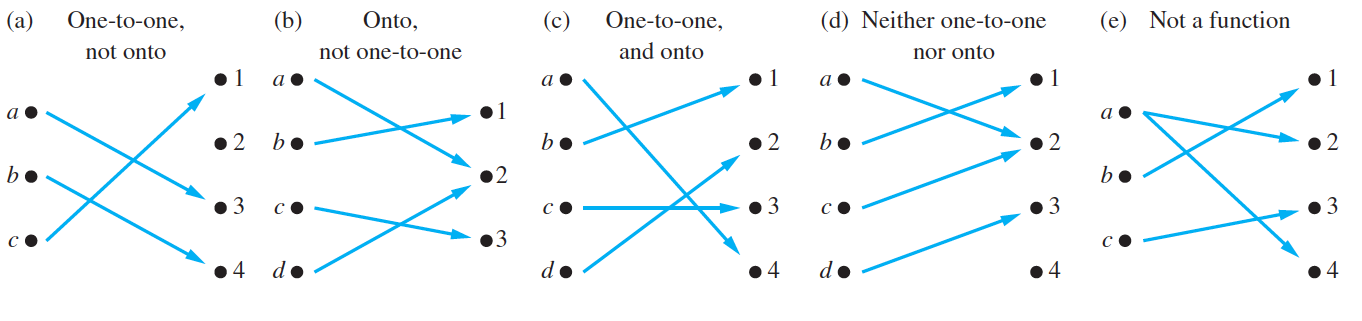
\includegraphics [width=6.5in]{Figure-2-3-5-TypesOfCorrespondences}
   \caption{Types Of Correspondences}
   \label{figure:Figure-2-3-5-TypesOfCorrespondences}
\end{figure}

    \subsection {Inverse of a Function}
    \begin{definition}[Inverse of a Function] \index{inverse of a function}
    Let $f$ be a One-to-One-Correspondence from the set $A$ to the set $B$. The inverse function of
$f$ is the function that assigns to an element $b$ belonging to $B$ the unique element $a$ in $A$
such that $f (a) = b$. The inverse function of $f$ is denoted by $f^{-1}$. Hence, $f^{-1} (b) = a$ when
$f (a) = b$.
    \end{definition}

\begin{definition}[Increasing and Strictly Increasing Functions]
A function $f$ whose domain and codomain are subsets of the set of real numbers is called \textit{increasing} if $f(x) \le f(y)$, and \textit{strictly increasing} if $f(x) < f(y)$, whenever $x<y$ and $x$ and $y$ are in the domain of $f$. (The word \textit{strictly} in this definition indicates a strict inequality.)
\end{definition}

\section {Composition of Functions}
\begin{definition} [Composition of Functions] \index{function composition}
Let $g$ be a function from the set $A$ to the set $B$ and let $f$ be a function from the set $B$ to the set $C$. The \textit{composition} of the functions $f$ and $g$, denoted by $f \circ g$, id defined by 
$$(f\circ g)(a)=f(g(a)).$$
\begin{notes}
Note that function composition is right-associative and that $f\circ g \ne g \circ f$. Note that the composition operator is a function which takes other functions as operands and returns a function. This is called treating functions as first-class objects in object oriented languags. Not all programming languages offer this ability.
\end{notes}
\end{definition}




\section {Common functions in computer science}

We are used to the functional notation of algebra
$$  g(x,y)$$
We are also accustomed to operators from programming languages
$$x+y$$
If the function g is defined as the sum of the two arguments, the two notations mean the same thing. The second form is called operation notation and works well for both binary and unary operators. But for arguments of more than 2 it is difficult to use. Note that the usual form is infix. But if we adopt a different convention, putting the operator after all the arguments, it is now possible to have functions of any number of arguments written in operator notation with no loss of precision. If the operator follows the operands, the notation is called post-fix. If the operator preceeds the operands, it is called prefix. Thus the function notation, prefix, infix, and suffix notation for addition are
$$+(a,b)$$
$$ab+$$
$$a+b$$
$$+ab$$
Note that the C language has a way of converting a symbol into an infix operator for a binary function.

We make special note of the important distinctions between common programming languages and the mathematical functions they implement. First, it is obvious that the mathematical convention of juxtaposing operands as implied multiplication does not work for computer languages which are not constrained to single character variables. Therefore the usual convention of an explicit multiplication operation, most always *, is adopted. Next is the challenge of differentiating between regular division and integer division. Several operators are employed in various languages and texts and sometimes is only implied by the type of the returned value. In many languages the type of the value to be returned value is infered by the types of the operands. Therefore an integer divided by an integer returns an integer, a case of integer division. To overcome this we see the apparently odd truth that $4/3 \ne 4.0/3$ in many languages. A more rigorous approach is delayed until the chapter on number theory but we define integer division in this chapter to connect the material more closely to contemporary coding practice.

	\subsection{Functions between Natural Numbers or Integers}
	\begin{displaymath}
	\text{Factorial}(n) = \prod_{i=1}^n i
	\end{displaymath}
	The remainder function is that function which returns the remainder when doing integer division. We will formally define this in the unit on Integers.
	
    \subsection {Functions of Real to Integer}
    
    \begin{definition} [Floor and Ceiling Functions]
    The \textit{floor function} assigns to the real number $x$ the largest integer that is less than or equal to $x$. The value of the floor function at $x$ is denoted by $\lfloor x \rfloor$. The \textit{ceiling function} assigns to the ral number $x$ the smallest integre that is greater than or equal to $x$. The value of the celing function at $x$ is denoted by $\lceil x \rceil$.
    
    The floor function is sometimes called the \textit{greates integer function}. It may be denoted by $[x]$. 
    \end{definition}
    
    
   \begin{table}[htbp]
   \centering
   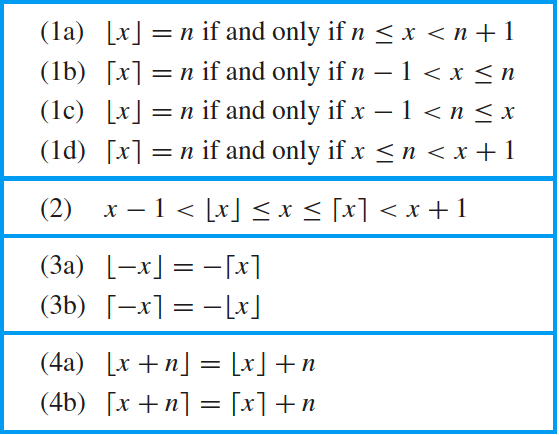
\includegraphics [width=3in]{Table-2-3-1-PropertiesOfFloorAndCeilingFunctions}
   \caption{Useful Properties of the Floor and Ceiling Functions}
   \label{table:UsefulPropertiesOfTheFloorAndCeilingFunctions}
   \end{table}

    

    \subsection{Functions between Boolean and Integer}
    ASCII is a 7-bit character set containing 128 characters. It contains the numbers from 0-9, the upper and lower case English letters from A to Z, and some special characters. The character sets used in modern computers, in HTML, and on the Internet, are all based on ASCII.
    
Boolean $\leftrightarrow$ Integer
\begin{table}[htbp]
   \centering
   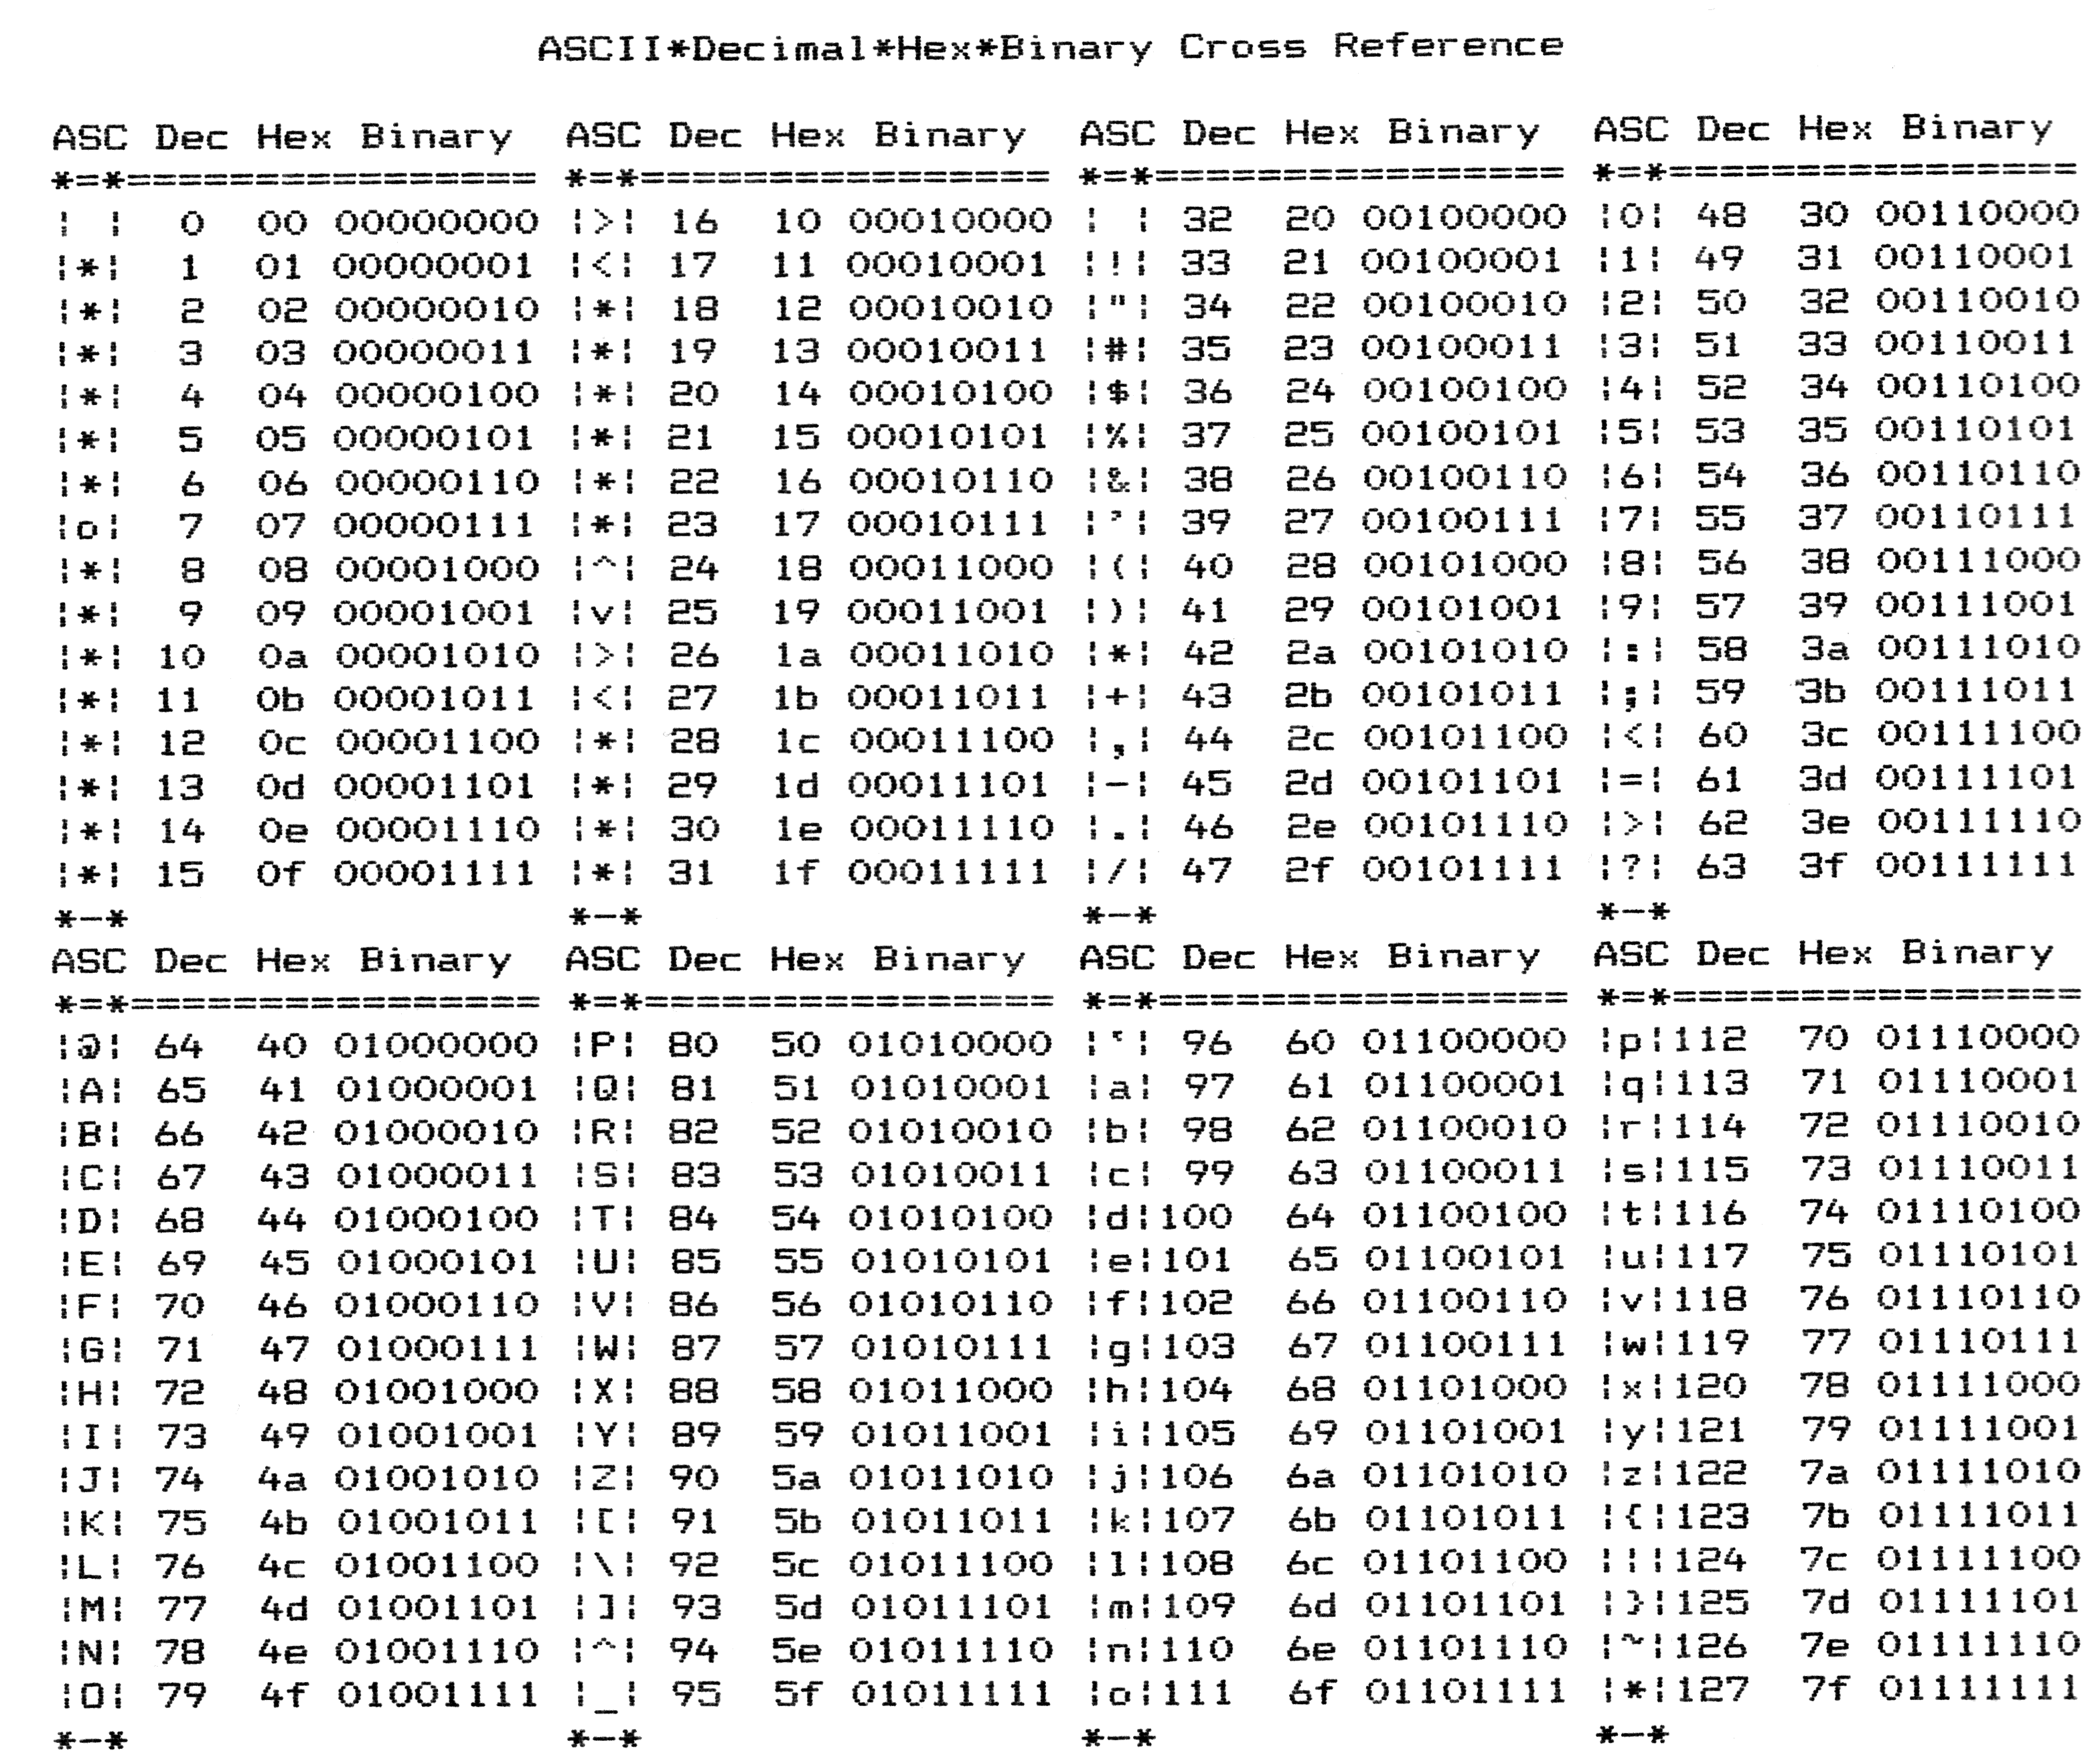
\includegraphics [width=5in]{asciifull}
   \caption{ASCII: American Standard Code for Information Interchange, 7-bit}
   \label{table:ASCIITable}
   \end{table}

    \subsection {Functions Between Boolean and Real}
Boolean $\leftrightarrow \mathbb{R}$ 

    \subsection {Functions of Real to Real}
polynomial, log, log-linear, exponential
increasing/decreasing versus strictly increasing and decreasing
cipher function
permutation function

	\subsection{Other Useful Functions}
	\begin{definition}[Characteristic Function]
	Let $S$ be a subset of a universal set $U$. The \textbf{characteristic function} $f_S$ of $S$ is the function from $U$ to the set $\mathbb{B}$ such that $f_S(x) =0$ if $x$ does not belong to $S$ and $f_S(x)=1$ when $x$ does belong to $S$.
	\end{definition}



\section {Composition of Functions}

Properties of Functions: Onto, One-to-One, One-to-One Correspondence, Invertible
An invertible function is called a permutation

Elementary Functions Used in Computer Science and Engineering
exponential and logarithmic, floor and ceiling, integer and absolute value, remainder function (MOD operator in programming), integer to binary and binary to integer, from natural numbers to integers.

It helps to note that when specifying function composition we begin to speak of the function like an operand. For example we can define a function $h$ as the composition of two other functions $f$ and $g$ using the composition operator. In functional notation we call this treating a function as a first class object, that is, the function is an object no different than other operands but simply drawn from the set of functions.

\begin{figure}[htbp]
   \centering
   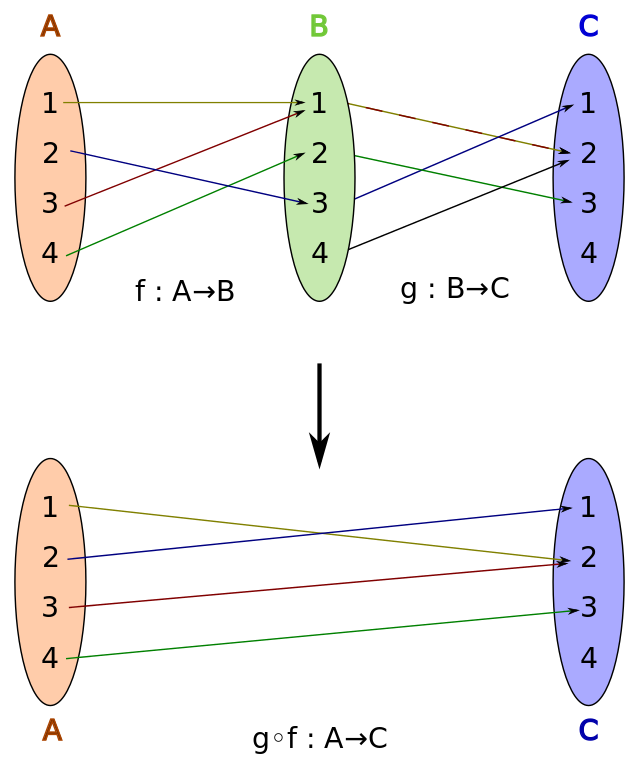
\includegraphics [width=3in]{Example_for_a_composition_of_two_functions}
   \caption{Function Composition}
   \label{figure:ExampleForACompositionOfTwoFunctions}
\end{figure}


subsection {Total and Partial Functions}
A total function is one that has a maplet for every element in the domain. These are called well defined functions. Some functions are undefined for some elements in the domain and these are called partial functions. Note that division on two numbers is a partial function. It is represented by an line through the arrow from domain to co-domain.

Not every element in the co-domain may be the image of an element in the domain. The set of all images is called the scope of the function.

\begin{definition}[Partial Function]\index{partial function}
A \textit{partial function} $f$ from a set $A$ to a set $B$ is an assignment to each element $a$ in a subset of $A$, called the \textit{domain of definition} of $f$ , of a unique element $b$ in $B$. The sets $A$ and $B$ are called the \textit{domain} and \textit{codomain} of $f$ , respectively. We say that $f$ is \textit{undefined} for elements in $A$ that are not in the domain of definition of $f$. When the domain of definition of $f$ equals $A$, we say that $f$ is a \textit{total function}. The notation $h:A \nrightarrow B$ is often used as a notation to designate a partial function $h$ that maps the set $A$ to $B$ where the set $A$ has undefined elements for the function $h$. However some authors use the same notation for partial functions as they do for partial functions.
\end{definition}



\section {Visual Representations of Functions: Set~mappings~and~analytic~geometry}
    In analytic geometry we speak of the graph of a function when we talk about ploting it against two or more axes. Note that in discrete math we will use the term \textit{graph} in a different way which does not mean the same thing.  
    
   \begin{figure}[htbp]
   \centering
   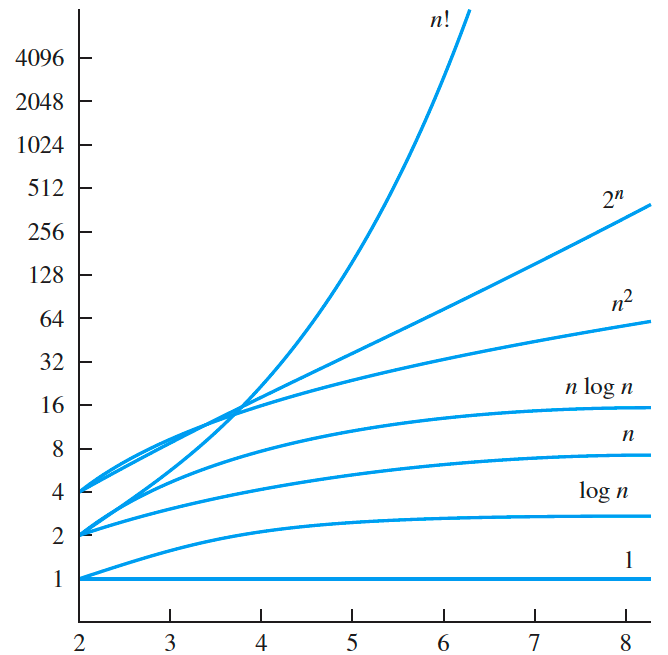
\includegraphics [width=4in]{Figure-3-2-3-GrowthOfFunctions}
   \caption{Graphs of Common Functions Needed In Computer Science}
   \label{figure:GraphsOfCommonFunctions}
\end{figure}

\section {Sequences}
Formally, a sequence can be defined as a function whose domain is either the set of the natural numbers (for infinite sequences) or the set of the first n natural numbers (for a sequence of finite length n). The position of an element in a sequence is its rank or index; it is the natural number from which the element is the image. It depends on the context or a specific convention, if the first element has index 0 or 1. When a symbol has been chosen for denoting a sequence, the nth element of the sequence is denoted by this symbol with n as subscript; for example, the nth element of the Fibonacci sequence is generally denoted $F_n$.

Like tuples, these are ordered lists. Unlike tuples, they vary in length and notation.

\begin{definition} [Sequence] \index{sequence}\index{term}
A \textit{sequence} is a function from a subset of the integers to a set $S$. We use the notation $a_n$ to denote the image of the integer $n$. We call $a_n$ a \textit{term} of the sequence. 

We use the notation $\{a_n\}$ to describe the sequence. Note how this conflicts with set notation. Note how there is no requirement that the set $S$ be numeric. We often describe sequences by listing the terms of the sequence in order of increasing subscripts.
\end{definition}

\begin{definition}[Geometric Progression]\index{geometric progression}\index{initial term}\index{common ratio}
A \textit{geometric progression} is a sequence of the form
$$ar^0,ar^1,ar^2, \dots ,ar^n, \dots$$
where the \textit{initial term} $a$ and the \text{common ratio} $r$ are real numbers.
\end{definition}

Sequences of the form $a_1, a_2, . . . , a_n$ where the terms are drawn from some set of symbols rather than numbers are often used in computer science. These finite
sequences are also called \textit{strings}. This string is also denoted by $a_1a_2 . . . a_n$. (Recall that bit strings, which are finite sequences of bits, were introduced in Section 1.1.) The length of a
string is the number of terms in this string. The empty string, denoted by $\lambda$, is the string that has no terms. The empty string has length zero.

\subsection{Special Integer Sequences}
A common technique needed in programming is finding an algorithm that will generate a particular sequence. This is the same as finding a function to do the same substituting the index variable for the loop counter. 

Trying to guess the function that can be used to create the sequence is a common test item. Note that an infinite number of sequences can be created that begin with the same few terms that are given. Still it is important to be able to quickly recognize the most common sequences and functions such as arithmetic and geometric progressions. 




In mathematics a \textit{finite sequence} is usually defined as any function $f$ whose domain is a finite initial set $\{1,2,3, \dots ,n\}$ of positive integers. The number $n$ of integers in the domain of $f$ is the \textit{length} of $f$. When considering $f$ as a finite sequence it is customery to write
$$f_1,f_2, \dots$$
rather than
$$f(1),f(2), \dots$$
in designating the value of $f$ at 1,2, \dots.

Along with this subscript notation there is the \textit{n-tuple} notation
$$(f_1,f_2, \dots f_n)$$


$f_i$ is the $i_{th}$ \textit{entry} or \textit{term} of $f$. This \textit{n-tuple} notation indicates how explicit short finite sequences can be defined and pictured. For example, the equation  
$$x=(5,1,4,0)$$
tells us that $x$ is the finite sequence of length 4 whose values on its domain \{1,2,3,4\} are given by
$$x_1=x(1)=5$$
$$x_2=x(2)=1$$
$$x_3=x(3)=4$$
$$x_4=x(4)=0$$

The most common domain for a sequence is $\mathbb{N}$. However it is frequently more convenient to use natural numbers including zero. There is an edge case where sometimes the domain is the null set in which case the sequence is empty and can be shown using a pair of empty parentheses to emphasize that there are no terms in the sequence
$$(  )$$

Consider a function $\sigma:\mathbb{N} \rightarrow \mathbb{Z}$
For example sigma(x)=2*x
this gives maplets 1|->2, 2|->4, etc
Since the domain is understood to be natural numbers it is easier to just write the images as a list:
2,4,6,8, etc
We can use subscript notation and state this more abstractly:

A sequence A is a(1),a(2),a(3),...a(i) 
or
$\{a(n) n \in N\}$  or even more compactly as $\{a(n)\}$ when it is understood we intend a sequence. It is common in sequences to base not strictly on natural numbers but natural numbers plus the member zero. 

Note that this definition of sequence allows for non-numeric sequences.



\begin{definition}[Geometric Progression]\index{geometric progression}
A \textit{geometric progression} is a sequence of the form
$$ar^0,ar^1,ar^2, \dots ,ar^n, \dots$$
where the \textit{initial term} $a$ and the \textit{common ratio} $r$ are real numbers.
\end{definition}

\begin{definition}[Arithmetic Progression] \index{arithmetic progression}
An \textit{arithmetic progression} is a sequence of the form
$$a+0d,a+1d,a+2d, \dots ,a+nd, \dots$$
where the \textit{initial term} $a$ and the \textit{common difference} $d$ are real numbers.
\end{definition}



   \begin{table}[htbp]
   \centering
   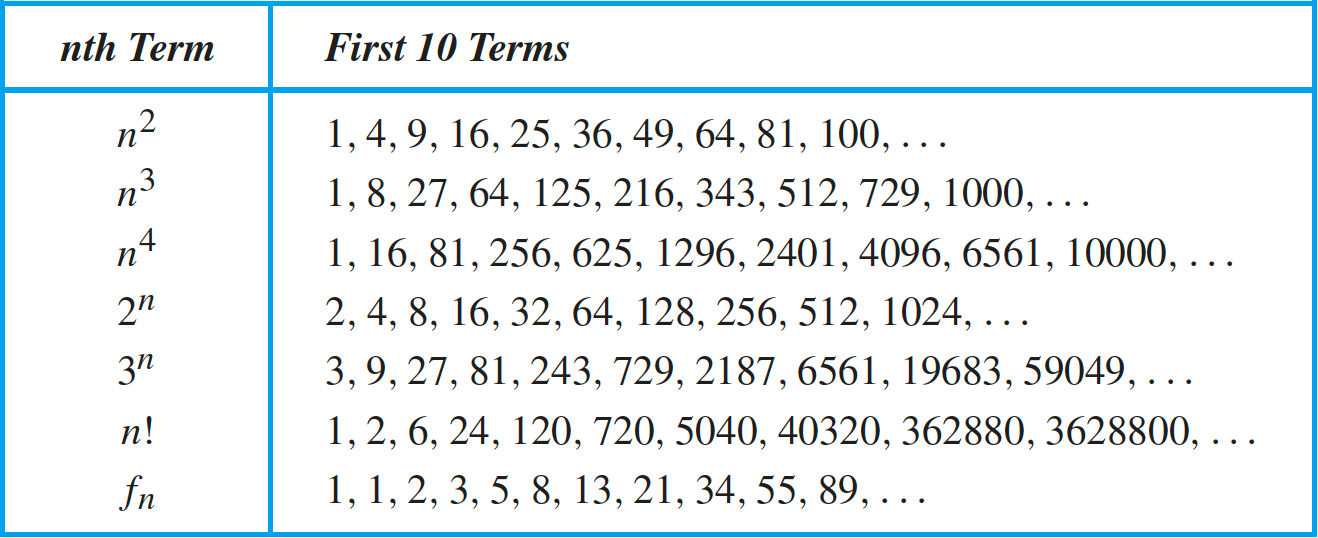
\includegraphics [width=5in]{Table-2-4-1-SomeUsefulSequences}
   \caption{Some Useful Sequences}
   \label{table:Some Useful Sequences}
   \end{table}

The reader interested in integer sequences will want to look at the Online Encyclopedia of Integer Sequences originally created by Neil Sloane and available online.

\subsection{Strings}
Sequences sometimes have a co-domain of symbols that can be listed in a sequence such that each symbol is a distinct symbol. This allows sequences of symbols to be represented without commas without confusion. The set of symbols is usually called the alphabet and commonly represented with the capital sigma, $\Sigma$. Finite equences of symbols are called strings and represented by $a_1a_2a_3 \ldots a_n$ 


\subsection{Evaluation of Functions}
Note that functions have one notation that just gives the function a name and identifies the domain and codomain but does not define how one maps to the image given the pre-image. 
Some functions are trivially evaluated. The other notation defines how that is done and it is often a mathematical expression. But it need not be. It can be any procedure that will ensure a value from the codomain is returned when requested. 

This has a historical point. Prior to the middle of the 20c the word computer was a job description not a machine. It was the job of the mathematician to give the computers the instructions on how to compute the functions that were needed. More often than not these values were compiled into books and used as reference when the function needed to be evaluated. Turing was one of the first to ask what limits a machine would have if the mathematician gave instructions that could be executed by a machine. We now call these procedures the algorithms that are used to evaluate a function given it aguments. 




\section {Sigma Notation, Summations and Open Form Formulas}
Given a function which produces a sequence, one operation we frequently wish to do is sum the terms. We define notation for this.

\begin{definition} [Summation] \index{summation}
Given a sequence $\{a_n\}$, we use the notation $\sum_{j=m}^{n} a_j $ to represent $a_m + a_{m+1}+ ... + a_n$. The variable $j$ is called the \textit{index of summation}, the value $m$ the  \textit{lower limit} and the value $n$ the \textit{upper limit}. 
\end{definition}

Shift the index of summation. 
Ex: What is the evaluation of $\sum_{j=1}^5 j^2$ with an index of summation that runs from 0 to 4 instead of 1 to 5? Substitute $k=j-1$ so the old index of summation would run from 1 to 5 but the new index of summation will run from  0 to 4 and the new summand will be $(k+1)^2$.
Sol: 

\subsection{Properties of Summation}

\begin{align}
\sum_{i=m}^n ca &=  c \sum_{i=m}^n a\\
\sum_{i=m}^n (a \pm b) &= \sum_{i=m}^n a \pm  \sum_{i=m}^n b \\
\sum_{i=m}^n a &= \sum_{i=m+p}^{n+p} a
\end{align}



It may start at something other than 1 and may sum to infinity. The letter $j$ is called the \textit{index of summation}, and the choise of the letter $j$ as variable is arbitrary; that is, we could have used any other letter, such as $i$ or $k$. Or, in notation, 
$$\sum_{j=m}^n a_j = \sum_{i=m}^n a_i = \sum _{k=m}^n a_k$$
where $m$ is the \textbf{lower limit} and $n$ is the \textit{upper limit}.

\subsection{Closed form solution}
For finite sequences, it is always possible to add the terms to calculate the sum. But these sequences can be very long making the summation an expensive operaton. And it is impossible if the sequence is infinite. Another way must be found and this brings us to closed form solutions. Many summations can be restated as formulas that are functions of the upper limit of summation. These are less burdensome computationally and are possible for infinite sequences with calculus.  
A closed form soluiton will have a finite number of operations and does not require the articulation of every term of the sequence.

\begin{theorem}
If $a$ and $r$ are real numbers with $r\ne 0$, then
\[   
\sum_{j=0}^n ar^j  = 
     \begin{cases}
       \frac{ar^{n+1}-a}{r-1}, &\quad\text{if $r \ne 1$,}\\ 
       $(n+1)a$,               &\quad\text{if $r=1$.} \\
     \end{cases}
\]
\end{theorem}

telescoping

\subsection{Useful Closed Form Solutions}
\begin{align}
\sum_{k=1}^n k & = \frac{n(n+1)}{2}\\
\sum_{k=1}^n k^2 & =\frac{n(n+1)(2n+1)}{6}\\
\sum_{k-1}^n k^3 & =\frac{n^2(n+1)^2}{4}\\
\sum_{i=0}^n 2^i & = 2^0+2^1+\dots 2^{n-1}+2^n= 2^{n-1} -1
\end{align}


\section {Growth of Functions and Asymptotic Notation}
As we saw when we talked about the graphs of common graphs  (Figure \ref{figure:GraphsOfCommonFunctions}) we see that there is a difference among these functions in how quickly the function values climb as the argument, $n$, grows. For example you know that a quadratic polynomial will overtake a linear polynomial. But many linear functions will evaluate to higher numbers for small values. We want some way to express the concept that a quadratic is in some sense bigger. This leads to a new notation, the Big-O or asymptotic notation or \textbf{Bachmann-Landau notation} and the $O$ is sometimes called the \textbf{Landau} symbol. Knuth extended this notation in his work.
Characterize functions according to their growth rates. different functions with the same growtwth rate may be represented using the same O notaiotn. the order of the function. O is used to specify an upper growth bound. Since a slower growing function may give a higher value for low values of the argument but pull ahead and forever remain ahead for large values, it is not sufficient to offer a few values to demonstrate. 

\begin{definition}
Let $f$ and $g$ be functions fromthe set of integers or reals to the set of real numbers. We say that $f(n)$ is $O(g(n))$ if there are constants $C$ and $k$ such that 
\begin{displaymath}
\lvert f(x)\rvert \le C\lvert g(n)\rvert
\end{displaymath}
whenever $n>k$. We read this as ``$f(n)$ is big-oh of $g(n)$''. The constants $C$ and $k$ are called the \textbf{witnesses} to the relationship $f(n)$ is to $O(g(n))$. To demonstrate that $f(n)$ is big-oh  we only need to produce one set of witnesses. Note that it is an abuse of the notation to say $f(n)=O(g(n))$ since no equality is established, only an assertion that the functions belong to the same class of functions. 
\end{definition}

$$f(n) = O(g(n)) \text{ as } n\rightarrow \infty$$
if and only if for all sufficiently large values of $n$, the absolute value of $f(n)$ is at most a positive constant multiple of another function $g(n)$. That is $f(n)=)(g(n))$ if and only if there existss a positive realy number C and a real number $n_0$ such that
$$\lvert f(n) \rvert \le cg(n) \text{for all } n\ge n_0$$
Instead of looking at at the function itself, it is helpful to look at a function as a family of functions. For a linear function $f(n)=n$ we can define a set of functions based on that by introducing constants $c_0$ and $c_1$ like this: $f(n)=c_1n+c_0$. This can be done for all the common functions giving us this list:\\
$
\begin{array}{lll}
\text{log} &  O (\log n) & \\
\text{log linear} & O(n \log n) & \\
\text{linear} & O(n)& c_1n+c_0\\
\text{quadratic} &On^2& c_2n^2 +c_1n + c_0 \\
\text{cubic}&O(n^3) & c_3n^3 + c_2n^2 + c_1n + c_0\\
\text{exponential} &O(2^n) & \\
\text{factorial} & O(n!) &
\end{array}
$

If there are constants such that a function can be restated as one of these families of functions then we say it is \textit{of the same order of magnitude} as 

Given two linear polynomial equations, we can always do this by changing the values of the constants. But no matter how you change the constants of a linear polynomial, a quadratic polynomial will always overtake it. This shows that a quadratic will ALWAYS beat a linear function, that they are in some sense in different categories regardless of the choice of constants. This gives us the concept of the category of the function or the order or magnitude designated by Big O. We can change any linear function into another linear polynomial function by changing the constants. We group all of these together and call them linear polynomial functions or polynomial functions on n, written O(n). We can prove that there are at least 7 categories that are important to the study of computer science, constant O(1), linear O(n), log O(log n), log-linear O(n log n), quadratic O(n**2), exponential O(2**n), and factorial O(n!). Note that each of these is a grouping of functions that include all the variations of different constants. By choosing the constants, we can always find some n sub 0 such that a quadratic will beat a linear. This gives us an ordering of these categories

$O(1) < O(\log n) < O(n) < O(n \log n) < O(n^2) < O(2^n) < O(n!)$

For any two specific functions of different categories one can find the n sub 0 at which the larger function overtakes the smaller and forever remains ahead. This way of viewing the relative size of functions will be used when we study the complexity of algorithms later.

\begin{theorem}
Let 
\begin{displaymath}
p(n)=a_kn^k+a_{k-1}n^{k-1}+\ldots +a_1n^1+a_0
\end{displaymath}
be a polynomial in $n$ of degree $k$, where each $a_i$ is nonnegative. Then
\begin{displaymath}
p(n)=\Theta(n^k).
\end{displaymath}
\begin{proof}

\end{proof}
\end{theorem} 


\begin{definition}[Big-Omega]
Let $f$ and $g$ be functions from the set of integers or reals to the set of reals. We say that $f(n)$ is $\Omega(g(n))$ if there are positive constants $C$ and $k$ such that 
\begin{displaymath}
\lvert f(n)\rvert \ge C\lvert g(n)\rvert
\end{displaymath}
whenever $x>k$. Read this as ``$f(n)$ is big-Omega of $g(n)$''.
\end{definition}

\begin{definition}[Big Theta]

\end{definition}

\newpage

	






                      %%% RELATIONS %%%
\chapter {Relations}
Relations support comparisons or connections between elements within a set or between two or more sets, or between members of the same set. For example ``less than or equal'', ``is perpendicular to'', ``is a cousin to'' are relations on a set of numbers, lines, or people. 

Relations are closely associated with functions but we looked at those first since you are familiar with them from before. Relations are a superset of functions, all functions are relations but not all relations are functions.

The fundamental restriction to a function is that it needed to evaluate to exactly one value. A relation can be a many-to-many mapping from the domain to the codomain. In its most abstract statement, all valid subsets of the cross product of the domain and codomain are relations.

A fundamental paradigm is one called objects/relations and is found in programming languages today. We saw that sets are collections of objects and we saw that predicates take on the value true when a particular property is found in that object. Objects can have relationships among them and the most basic is the binary relationship. In a binary relationship we way that the two objects either are in or not in that relationship with each other. This chapter explores the consequences of this and its many applications.



\section {Relations}
\begin {definition}[Binary Relations]\index{binary relations}
Let $A$ and $B$ be sets. A \textit {binary relation $\mathrel{R}$ between $A$ and $B$} is a subset of the Cartesian Product $A \times B$. We can denote the binary relation on two elements $a$ and $b$ by $a\mathrel{R}b$, or by $(a,b)\in \mathrel{R}$. We can denote the lack of relationship $\mathrel{R}$ between the two elements with the notation $a\not\mathrel{R}b$ or $(a,b) \not \in R$. The sets $A$ and $B$ may be the same set in which case we say $\mathrel{R}$ is a relation on $A^2$ or on the set $A$. We read ``a is in relation to b'' or ``a is related to b'' to indicate they are related. \\

Relations are not limited to relations on two sets but can be applied to any number of sets. The relation is still defined as a subset of the n-tuples formed from the cross product of the sets.

Relations are sets of tuples of the cross product and set operators can be used on them.

Given a set $A$, the relation $\{(a,a)|a\in A\}$ is the equality or identity relation and is denoted by $\Delta_A$.
\end {definition} 

Note that functions are a subset of relations. Note that plotting graphs of functions uses the Cartesian plane which is a relation of $\mathbb{R}^2$. 

\subsection{Inverse Relation}
The \textit{inverse of a relation} $\mathrel{R}$ from set $A$ to $B$ is the relation denoted by $R^{-1} = \{(b,a)|(a,b)\in \mathrel{R}\}$.

    \subsection {Relational operators}
    Equality, inequality, greater than, greater than or equal, less than, less than or equals are all relational operators that every programmer learns. To these we introduce one that is not often seen in programming, the divides relation.
    
    \begin{definition}[Divides]\index{divides}
    If $a$ and $b$ are integers with $a\ne 0$, we say that \textit{$a$ divides $b$} if there is an integer $c$ such that $b = ac$, or equivalently $\frac{b}{a}$ is an integer. When $a$ divides $b$ we say that $a$ is a factor or divisor of $b$, and that $b$ is a multiple of $a$. The notation $a \mid b$ denotes that $a$ divides $b$. We write $a\nmid b$
when $a$ does not divide $b$.
    \end{definition}


\section {Properties of Relations}
    \begin {definition}[reflexive relation]\index{reflexive relation}
    A relation $R$ on a set $A$ is called \textit{reflexive} if $(a,a) \in R$ for every element $a \in A$. The relation $R$ is reflexive if $\forall a((a,a) \in R)$.
    \end {definition}
    
    \begin {definition}[Symmetric Relation]\index{symmetric relation}
    A relation $R$ on a set $A$ is alled \textit{symmetric} if $(b,a) \in R$ for all $a,b \in A$.
    \end {definition} 
    
    \begin {definition}[Antisymmetric]\index{antisymmetric}
    A relation $R$ on set $A$ such that for all $a,b \in A$, if $(a,b) \in R$ and $(b,a) \in R$, then $a=b$ is called \textit{antisymmetric}
    \end {definition}
    
    \begin {definition}
    A relation $R$ on a set $A$ is called \textit{transitive} if whenever $(a,b)\in R$ and $(b,c) \in R$, then $(a,c) \in R$. The relation $R$ on a set $A$ is transitive if we have $\forall a \forall b \forall c (((a,b) \in R \land (b,c) \in R) \rightarrow (a,c) \in R)$
    \end {definition}
    
    \begin{definition}[Anti-Reflexive Relation]\index{anti-reflexive relation}
    \end{definition}


\section {Composition of Relations}
Combining Relations in Rosen

\begin{definition}[Composition of Relations]\index{composition of relations}
Let $R$ be a relation from set $A$ to set $B$ and $S$ a relation from $B$ to a set $C$. The \textit{composite} of $R$ and $S$ is the relation consisting of ordered pairs $(a,c)$ such that $(a,b) \in R$ and $(b,c) \in S$. We denote the composite of $R$ and $S$ by $S \circ R$.
\begin{notes}
Carefully note the order of the operand in the composition operation.
\end{notes}
\end{definition}


\section {Graphic Representation of Relations}
For relations onto themselves, this gives what we will later call a directed graph. We cover graphs more formally in a later chapter.
    \subsection {Digraphs}
    A convenient pictorial representation of relations is to represent the domain and co-domain as ovals with the elements labeled. A pair that is in the relation is then represented by an arc from the element in the domain to the element in the co-domain. When the co-domain is the same as the domain the oval is sometimes omitted. We call this a \textit{directed graph}. We will cover directed graphs more formally in the chapter on Graphs.  

\section {Closure Property of Relations}
   \subsection {Transitive Closure of Relations}
   
   \begin{definition}
   Let $R$ be a relation on a set $A$. The \textit{connectivity relation $R^*$} consists of the pairs $(a,b)$ such that there is a path of length one from $a$ to $b$ in $R$.
   \end{definition}
   \subsection {Kleene Closure and Order}

\section {N-ary Relations}
We have only spoken of binary relations up to now. But more than two elements can be in a relation. 
\begin{definition}
Let $A_1,A_2, \dots ,A_n$ be sets. An \textit{n-ary relation} on these sets is a subset of $A_1 \times A_2 \times \dots \times A_n$. The sets $A_1,A_2, \dots ,A_n$ are called the \textit{domains} of the relation, and $n$ is called its \textit{degree}.
\end{definition}

\begin{definition}
Let $R$ be an $n$-ary relation and $C$ a condition that elements in $R$ may satisfy. Then the \textit{selection operator $s_C$} maps the $n$-ary relation $R$ to the $n$-ary relation of all $n$-tuples from $R$ that satisfy the condition $C$.
\end{definition}

\begin{definition}
The \textit{projection} $P_{i_1i_2, \dots ,i_m}$ where $i_1 < i_2 < \dots i_m$, maps the $n$-tuple ($a_1,a_2, \dots , a_n$) to the $m$-tuple ($a_{i_1},a_{i_2}, \dots ,a_{i_m}$), where $m \le n$.
\end{definition}

    \subsection {Application to Databases}

\section {Matrices and Linear Algebra}
Many include matrices in Discrete Mathematics. We exclude this since it is offered as a separate course.











\section{Representations of Relations}
The definition of relations are as a subset of the cross product $A \times B$. But two alternate representations of relations are useful.
  \subsection{Representing Relations Using Matrices}
  Given a subset of $A \times B$, one can represent the relation by creating a matrix with the elements of the sets $A$ and $B$ along the two axes of the matrix and entering a 1 when that pair is in the relation and 0 if not. 
  
  
  
  \subsection{Representing Relations Using Digraphs}
  \subsection{Paths in Directed Graphs}

\section{Closures on Relations}
  \subsection{Closures}
Sometimes an operation will return something that is outside the set from which the argument was drawn. For example, you can perform division on two integers but not get an integer as a return value. You can solve an equation like $2\cdot 2x+1=0$ with 2 and 1 both being valid rational numbers yet find you have a number that is outside the set of rational numbers. We say that the set is not closed under these operation                                  s. 

When we look at the properties of relations sometimes we see that a given relation is closed, that is every pair needed to satisfy that relation are found in the relation. When we find that to be true, we say the set is closed under that relation.

Let $R$ be a relation on a set $A$. $R$ may or may not have some property \textbf{P}, say reflexivity. If the set $A$ does not possess the property, it is possible to add pairs to the relation such that the union of the two relations (which after all are just sets of pairs) will possess that property. We are now ready to offer a formal definition.

\begin{definition}[Closure]\index{closure}
A set that is closed under an operation or collection of operations is said to satisfy a closure property. When a set $S$ is not closed under some operations, one can usually find the smallest set containing $S$ that is closed. This smallest closed set is called the closure of $S$ (with respect to these operations). For example, the closure under subtraction of the set of natural numbers, viewed as a subset of the real numbers, is the set of integers. The closure of a set $S$ which does not posses the closure property under the reflexion relation can be created by summing the relation with all pairs that make the relation reflexive.
\end{definition}
The reflexive closure of a relation$R$can be formed by adding to $R$ all pairs of the form $(a,a)$with$a\in A$,not already in$R$. The addition of these pairs produces a new relation that is reflexive, contains$R$,and is contained within any reflexive relation containing $R$. We see that the reflexive closure of $R$ equals $R \cup \Delta$, where $\Delta=\{(a,a)\vert a\in A\}$is the diagonal relation on$A$.
 
  \subsection{Transitive Closures}

\begin{definition}
Let $R$ be a relation on a set $A$. The \textit{connectivity relation $R^*$} consists of the pairs $(a,b)$ such that there is a path of length at least one from $a$ to $b$ in $R$.
\end{definition}

\begin{theorem}
The transitive closure of a relation $R$ equals the connectivity relation $R^*$.
\end{theorem}

\begin{lemma}
Let $A$ be a set with $n$ elements, and let $R$ be a relation on $A$. If there is a path of length at least one in $R$ from $a$ to $b$, then there is such a path with length not exceeding $n$. Moreover, when $a \ne b$, if there is a path of length at lteast one from $R$ from $a$ to $b$, then there is such a path with length not exceeding $n-1$.
\end{lemma}

  \subsection{Computing Transitive Closures} 
  The most well known algorithm to compute the transitive closure of a relation is Warshall's Algorithm.

 
\section {Equivalence Relations}
reflective, symmetric, transitive
remainder function partitions

    \subsection {Equivalence Classes and Set Partitions}

\begin{definition}
The elements $a$ and $b$ that are related by an equivalence relatin are called \textit{equivalent}. The notation $a \sim b$ is often used to denote that $a$ and $b$ are equivalent elements with respect to a particular equivalence relation.
\end{definition}

\begin{definition}
Let $R$ be an equivalence relation on a set $A$. The set of all elements that are related to an element $a$ of $A$ is called the \textit{equivalence class} of $a$. The equivalence class of $a$ with respect to $R$ is denoted by $[a]_R$. When only one relation is under consideration, we can delete the subscript $R$ and write $[a]$ for this equivalence class.

If $b \in [a]_R$, then $b$ is called a \textbf{representative} of this equivalence class.
\end{definition}


\begin{theorem}
Let $R$ be an equivalence relation on a set $A$. These statements for elements $a$ and $b$ of $A$ are equivalent:
\begin{enumerate}[label=(\roman*)]
\item
$aRb$
\item
$[a]=[b]$
\item
$[a] \cap [b] \neq \emptyset$
\end{enumerate}
\end{theorem}

\begin{theorem}
Let $R$ be an equivalence relation on a set $S$. Then the equivalence classes of $R$ form a partition of $S$. Conversely, given a partition $\{A_i | i \in I\}$ of the set $S$, there is an equivalence relation $R$ that has the sets $A_i, i \in I$, as its equivalnece classes.
\end{theorem}

    \subsection {Partial Ordering Relations}
\begin{definition}[Posets]\index{poset}\index{partial order}
A relation $R$ on a set $S$ is called a \textit{partial ordering} or \textit{partial order} if it is reflexive, antisymemetric, and transitive. A set $S$ together with a partial ordering $R$ is called a \textit{partially ordered set} or \textit{poset}, denoted by $(S,R)$. Members of $S$ are called \textit{elements} of the poset.
\end{definition}

Many different relations on sets create posets such as $\ge$, evenly divides (|), and $\subset$. We create a new relation symbol $\preceq$.

\begin{definition}
Given a poset $(S,R)$ and two elements $a$, $b$, we use the notation $a \preceq b$ to indicate that $(a,b)\in R$. We use $\preceq$ to designate any relation of a poset. The elements $a$ and $b$ of a poset $(S,\preceq)$ are called \textit{comparable} if either $a\preceq b$ or $b\preceq a$. When $a$ and $b$ are selements of $S$ such that neither $a \preceq b$ nor $b \preceq a$, $a$ and $b$ are called \textit{incomparable}. If $a \preceq b$ and $a \neq b$, we use the notation $a \prec b$.
\end{definition}

\begin{notes}
Object oriented programming languages allow you to code relations. Note that since two elements of a set may be incomparable given the relation $\preceq$, we call it a partial ordering.
\end{notes}
    
\begin{definition}
If $(S,\preceq)$ is a poset and every two elements of $S$ are comparable, $S$ is called a \textit{totally ordered} or \textit{linearly ordered set}, and $\preceq$ is called a \textit{total order} or a \textit{linear order}. A totally ordered set is also called a \textit{chain}.
\end{definition}

\begin{definition}[Well-Ordered Set]\index{well-ordered set}
The poset $(S,\preceq)$ is called a \textit{well-ordered set} if it is a poset such that $\preceq$ is a total ordering and every nonempty subset of $S$ has a least element, (something defined in a few sections).
\end{definition}

\begin{theorem} [The Principle of Well-Ordered Induction]
Suppose that $S$ is a well-ordered set. Then $P(x)$ is true for all $x \in S$, if
INDUCTIVE STEP: For every $y\in S$, if $P(x)$ is true for all $x\in S$ with $x \prec y$, then $P(y)$ is true.
\begin{proof}
Suppose it is not the case that $P(x)$ is true for all $x\in S$. Then there is an element $y\in S$ such that $P(y)$ is false. Consequently, the set $A=\{x\in S | P(x) is false \}$ is nonempty. Because $S$ is well ordered, $A$ has a least element $a$. By the choice of $a$ as a least element of $A$, we know that $P(x)$ is true for all $x\in S$ with $x\prec a$. This implies by the inductive step $P(a)$ is true. This contradiction shows that $P(x)$ must be true for all $x\in S$.
\end{proof}
\begin{notes}
We do not need a basis step in a proof using the principle of well-ordered induction because if $x_0$ is th eleast element of a well ordered set, the inductive step tells us that $P(x_0)$ is true. This follows because there are no elements $x\in S$ with $x\prec x_0$.
\end{notes}
\end{theorem}


    \subsection {Lexicographic Order}\index{lexicographic order}
You may have already noticed that the way words get arranged in a dictionary are different than the way they would be sorted if they were numbers. This ordering of strings is called a lexicographic ordering. Consider two posets $(A_1,\preceq_1)$ and $(A_2,\preceq_2)$. The \textbf{lexicographic ordering} $\preceq$ on $A_1 \times A_2$ is defined by specifing how one pair, $(a_1,a_2)$ is less than another $(b_1,b_2)$. We say $(a_1,a_2) \prec (b_1,b_2)$ if either $a_1 \prec_1 b_1$ or if both $a_1= b_1$ and $a_2 \prec b_2$.

\begin{notes}
This came from Rosen. why are there two different relationships in this presentation?
\end{notes} 

\begin{definition}[Lexicographic Ordering]
Given strings $a_1a_2 \dots a_m$ and $b_1b_2 \dots b_n$ on a partially ordered set $s$. Suppose these strings are not equal. Let $t$ minimim of  $m$ and $n$. We define the string $A$ as less than $B$ if and only if
$$(a_1,a_2, \dots ,a_t) \prec (b_1,b_2, \dots ,b_t),$$
or
$$(a_1,a_2, \dots ,a_t) = (b_1,b_2, \dots ,b_t) \land m<n$$
\end{definition}

    \subsection {Haase Diagrams}\index{Haase diagram}
Consider Figure 9-6-3a of a small poset $(\{1,2,3,4,6,8,12\}, |)$. This Recall that a poset is a partial ordering and that means it is reflexive, anti-symmetric and transitive. If we know that the di-graph is of a poset we can then remove the reflexive edges. This gives us Figure 9-6-3b which has the reflexive edges removed. Since we know it must also be transitive we can safely remove those edges as well. If we use the convention that vertices that are "less than" in the ordering be placed lower on the graph we can also remove the directed edges and replace them with undirected edges. This gives Figure 9-6-3c which is known as a Haase Diagram or ordering diagram and represents the poset in an economical visual fashion.

   \begin{table}[htbp]
   \centering
   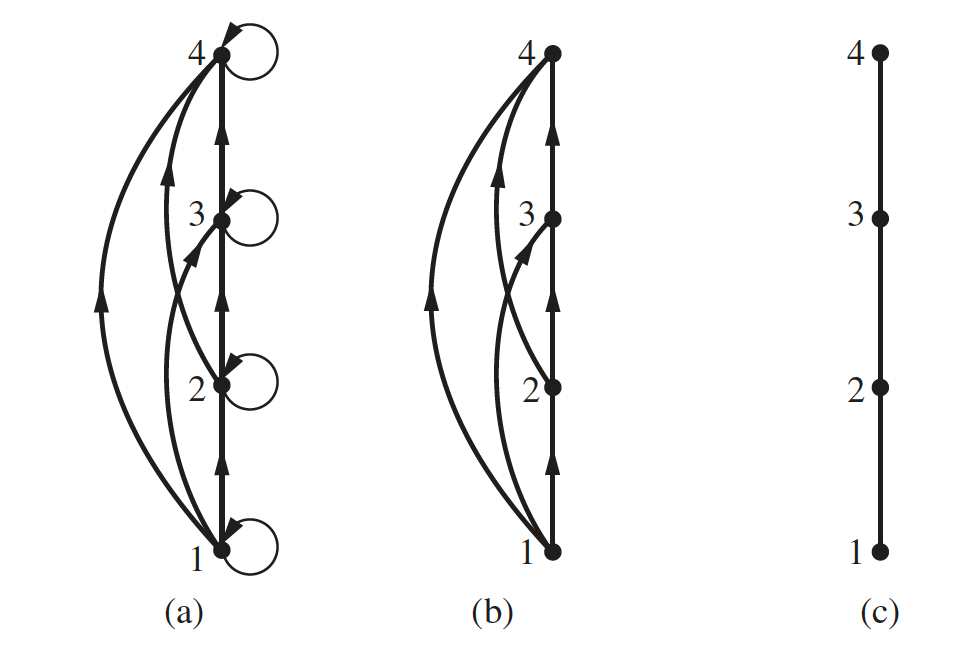
\includegraphics [width=3in]{Figure-9-6-2-ConstructionOfHaaseDiagram}
   \caption{Construction of a Hasse Diagram }
   \label{figure:Construction of a Hasse Diagram }
   \end{table}


    \subsection {Maximal and Minimal Elements}
When discussing the basic axioms of arithmetic that a student can assume in proofs, we introduced the Completeness Property (Definition \ref{CompletenessProperty}). We now add to that.

Posets have properties that are useful to some applications, in particular maximal and minimal elements. 

\begin{definition}[Upper and Lower Bounds]
An element of  a poset is called maximal if it is not less than any element o f the poset. That is, $a$ is \textbf{maximal} in the poset $(S,\preceq)$ if there is no $b\in S$ such that $a \prec b$. Similarly, an element of a poset is called minimal if it is not greater than any element of the poset. That is, $a$ is \textbf{minimal} if there is no element $b\in S$ such that $b \prec a$. Maximal and minimal elements are the top and bottom elements in a Haase Diagram.

If an element $a$ is called the \textbf{greatest element} of the poset $S$ if $b\preceq a$ for all $b \in S$. The greatest element is unique when it exists. Likewise, an element is called the least element if it is less than all the other elements in the poset. The element $a$ of a poset is the \textbf{least element} of $(S,\preceq)$ if $a\preceq b$ for all $b\in S$. The least element is unique when it exists.
\end{definition}

\begin{definition}[Least Upper Bound]\index{least upper bound}
The element $x$ is called the \textbf{least upper bound} of the subset $A$ if $x$ is an upper bound that is less than every other upper bound of $A$. Because there is onlyu one such element, if it exists, it makes sense to call this element \textit{the} least upper bound. That is, $x$ is the least upper boundf of $A$ if $a\preceq x$ whenever $a \in A$, and $x \preceq z$ whenever $z$ is an upper bound of $A$. Similarly, the ...
We denote these as glb($A$) and lub($A$). 
\end{definition}

\subsection{Lattices}
\begin{definition}[Lattice]\index{lattice}
A partially ordered set in which every pair of elements has both a least upper bound and a greatest lower bound is called a \textbf{lattice}.
\end{definition}

    \subsection {Topological Sorting}
\begin{definition}[Topological Sort]\index{topological sort}
A total ordering $\preceq$ is said to be \textbf{compatible} with the partial ordering $R$ if $a \preceq b$ whenever $aRb$. Constructing a compatible total ordering from a partial ordering is called \textbf{topological sorting} or as some mathematicians will say, a linearization of a partial ordering.
\end{definition}

\begin{lemma}\label{ExistenceOfMinimalElementInAPoset}
Every finite nonempty poset $(S,\preceq)$ has at least one minimal element.
\end{lemma}



\section{$n$-ary Relations and Their Applicaiton for Databases}
An innovation of database technology was the application of relations.

\begin{definition}
Let $A_1,A_2,\ldots,A_n$ be sets and an $n$-ary relation on these sets as a subset of $A_1\times A_2\times \ldots \times A_n$. The sets $A_1,A_2, \ldots, A_n$ are called the domains of the relation, and $n$ is called its \textit{degree}.
\end{definition}

Let the terms of the $n$-tuple represent datafields. Then each domain is a set of values that the datafield can take on. Each tuple in the relation can be treated like a record in a data processing system and the collection of them can be presented in a table where each column represents each of the elements drawn from the domains. By putting them into an $n$-tuple, we establish a relationship among those elements. We call this part of a relational data model. 

Often the fields have a functional relation to one or more other elements. That is, given the key field, the other element in the domain is uniquely determined. When such a functional relationship exists from one of the domains to another, we say the pre-image is the key to the table. If this holds for all the terms in the tuple we call this field the primary key for the table. 

We define an operation on a table called selection:
\begin{definition}
Let $\mathrel{R}$ be an $n$-ary relation and $C$ a predicate that elements of $\mathrel{R}$ may satisfy. Then the selection operator $s_c$ maps the $n$-ary relation $\mathrel{R}$ to the $n$-ary relation from $\mathrel{R}$ of all $n$-tuples from $\mathrel{R}$ that satisfy the predicate C.
\end{definition}
 
\newpage



	                      %%% ALGORITHMS %%%
\chapter {Algorithms}
Relative to many texts on discrete math, this chapter is sparse because most of the material overlaps with a standard undergraduate course that will focus on algorithms and their analysis. The emphasis for these notes is simply the mathematical concept and its relationship to the structures needed to approach computation from a theoretical perspective.

Function definitions must determine a unique value for the argument(s) given. While mathematical formulas are common, they are not required. What IS required is a definite process by which one finds the value in the co-domain to return as the function.

Consider that the argument does not need to be a single value. It can be a structure such as a sequence. The function can be on that sequence and return another sequence that possess some property. The classic example is a sort of that sequence. The input is some perhaps unsorted sequence and what is returned has the property that each element of the sequence is less than or equal to the ones later in the sequence. This is the beginning point for the study of those processes which defines functions like sort.

A pre-requisite to this class is at least one programming course so the student is expected to understand the conventions of a procedural language used to describe an algorithm. There is no universal way to describe an algorithm since programming languages will often use different ways of doing the same thing. The conventions of this book come from Rosen which represents a common notation that uses conventions from mathematics as well as programming languages.

\begin{definition}[Definition of Algorithm from Rosen]
An \textit{algorithm} is a finite set of precise instructions for performing a computation or for solving a problem.
\end{definition}
\begin{definition}[Definition of Algorithm from Schaums]
An algorithm $M$ is a finite step-by-step list of well-defined instructions for solving a particular problem, for instance to evaluate a function $f$ given an argument $X$ where $X$ may be any mathematical structure. Frequently there may be more than one algorithm to computer $f(X)$ and we need tools to analyze the differences between the different algorithms.
\end{definition}

\begin{definition}[PseudoCode]\index{pseudocode}
Pseudo code is a form of non-fiction prose that attempts to provide a rigorous definition of an algorithm using a natural language. Computer languages such as C or Algol are formal languages that conform to a syntax that allows them to be translated into computer code. But when discussing algorithms the overhead of those formal languages does not help understanding. 

The assignment statement will perform a binding of a value to a variable, called a state transition. Most computer languages use the equal sign (=) to indicate assignment. That is unfortunate since it is easy to confuse it with the equality relationship  operator which must use a different operator (typically == in many popular languages). Historically there are two other symbols used to indicate assignment including ":=" and "$\leftarrow$". 

Originally algorithms only needed to be understood by a human who had the job title of computer. The other statements should be easily understood by a student who has taken a programming course. 
\end{definition}

\begin{algorithm}
\caption{Finding the Maximum Element in a Finite Sequence}\label{base b}
\begin{algorithmic}[1]
\Procedure{max}{$a_1,a_2, \dots a_n$: integers}
\State $max\gets a_1$
\For{$i\gets 2, n$}\Comment{We have the answer if r is 0}
\If {$max < a_i$}
   
    \State $max\gets a_i$
    \EndIf
\EndFor\label{xxx} \\
\Return{$max$}
\EndProcedure
\end{algorithmic}
\end{algorithm}




\begin{algorithm}
\caption{Constructing Base $b$ Expansions}\label{base b}
\begin{algorithmic}[1]
\Procedure{base b expansion}{$n$: positive integer}\Comment{The g.c.d. of a and b}
\State $q\gets n$
\State $k\gets 0$
\While{$q\not=0$}\Comment{We have the answer if r is 0}
\State $a_k\gets q \bmod b$
\State $q\gets \lfloor q/b\rfloor$
\State $k\gets k+1$
\EndWhile\label{xxx} \\
\Return{$(a_{k-1} \dots a_1a_0)_b$}
\EndProcedure
\end{algorithmic}
\end{algorithm}

\section{Searching Algorithms}
\section{Sorting Algorithms}


\section{Topological Sort Algorithm}
\begin{algorithm}
\caption{Topological Sorting}\label{TopologicalSort}
\begin{algorithmic}[1]
\Procedure{topological sort}{$(S,\preceq)$: a finite poset}\Comment{}
\State $k\gets 1$
\While( $S \neq \emptyset$)
  \State $a_k \gets$ a minimal element of $S$  \Comment{guaranteed to exist by Lemma \ref{ExistenceOfMinimalElementInAPoset} }
  \State $S \gets S - \{a_k\}$
  \State $k \gets k+1$
\EndWhile
\Return{$a_1,a_2, \dots ,a_n$}  \Comment {a compatible total ordering of $S$}
\EndProcedure
\end{algorithmic}
\end{algorithm}



\section{The Halting Problem}
As a practical matter we know that programs that do not halt are of little use when it comes to computing functions. At a theorectical level it is interesting to consider whether it would be possible to construct a compiler that could recognize a program that would not halt. This leads us to this famous theorem of computer science.

\begin{theorem}[Halting Problem]
There is no algorithm that accepts an algorithm and some input data set as input and determines whether it will halt.
\end{theorem}

Every function has a method by which a value can be calculated. This often comes from calculus for many of the functions used in engineering but not always. For example we have a way of calculating the factorial function that uses only basic arithmetic. Regardless of how it is calculated you will note that they all have very specific steps that must be executed in some order that are well defined. This is called an algorithm. Computer science began with the proof that any well defined algorithm could be mechanically executed by a machine instead of a human. The term computer originally meant a human using computation tools like an adding machine to execute the steps needed to determine the values. These values of the functions were published in books and the function was evaluated by a lookup in a table instead of on-the-spot calculation.

Not all functions take in single parameters. Some, like the permutation function, will take in a large number of values and produce some permutation of those numbers. Sorting is just such a function. Clearly the work done by the sorting function will depend on the size of the input set which we call n. 

For practical reasons, we are interested in how long an algorithm will take given a particular set of numbers as input. This becomes a different function T for this algorithm which has as input the size of the input set, n. The time a specific algorithm will work on a particular input set before giving a result is the functionT(n). You might naively assume that T(n) will always result in the same value for any size input but you would be wrong. The T function will vary with both the size but also the specific input. For example some sort algorithms will have T(n) in the category of O(n) for sorted input but O(n**2) for out of order input. The big O of the algorithm will vary with the algorithm and its input.

While we are sometimes interested in the best-case scenario for the algorithm and its input set, we most often are more interested in the worst case scenario. What will be the big O for this algorithm over all the possible inputs it could get? This defines an upper bound for the complexity of this algorithm. Since the worst and best case for an algorithm may have functions from different categories, the best case may be in a different big O category. When analyzing algorithms, we call this the lower bound for that function on T(n). We give this the name Omega. When we find one category that contains both the upper and lower bound, we call this the Theta of that function. When we find a Theta for an algorithm we say we have found the tight upper bound 

We defer the further study of algorithmic complexity to your course on Algorithms in your undergrad program.


\section {Analysis of Algorithms}
This section overlaps with a course usually required on the analysis of algorithms. We attempt to limit the material here to only the most basic concepts. 
  \subsection{The Time Function of an Algorithm}
  We want to analyze how long an algorithm takes, called the time complexity of the algorithm. First note that many algorithms will use different numbers of steps depending upon the input they are given. So this is not a fixed function from algorithm to time but instead a range of values. The time might be computable for specific algorithm and a specific input but in general what we want is the range of possible times for this algorithm. Of all the possible ways we can analyze the performance of an algorithm the most basic is to look at the relationship between the ``size'' of the input and the time ignoring all other considerations. We represent this ``size'' as $N$. We call the time function $T$ so we want to perform asymptotic analysis on the function $T(N)$. You might naively expect that a given algorithm will have a fixed relationship to the size of the input but that is wrong. Sorting algorithms in particular will have different time functions for the same size input but input in different orders. This complicates the analysis of the time function of an algorithm and gives us a range of functions.
  
We know that a computer does not perform all instructions with the same amount of time. A division function will be slower than a move instruction. But the relationship between the time and the instruction can be set at a max and all instructions treated as the same length. This is not useful for predicting how long the algorithm will take but it can be used to determine the order of magnitude since the fixed multiple will not impact the growth. With this in mind, we simply count how many times each instruction is executed by the algorithm with no consideration for the actual time the computer will take with each one. 

Given this range, we might be interested in the best possible time, the worst possible time and/or the average time this algorithm will use over some set of input values. The most frequently analyzed is the worst case time and we present how that is described. We will use asymptotic function analysis (chapter on functions) to do this. 

While it is true that the time required to execute an instruction varies with the machine and even within a machine the instruction to be executed. For example a divide instruction is longer than a move. But this relationship is fixed, for the most part, and can be ignored for the purposes of asymptotic analysis. 

The most common analysis is relative to the economic reality of time. But a comparable analysis can be done for space requirements too. In fact any resource needed to run the algorithm can be subjected to analysis in a comparable way.

Since time functions will vary in their order based on the input, we are often asked to consider the best case and worst case performance of these algorithms when presented with input. It is common with sorting algorithms that the best case and worst case will be of different orders. It is often trivial to say that a given function $g$ is of a higher order, for example a quartic polynomial will beat a quadratic, but we often want to know the LEAST upper bound function. To do the analysis we must have a concept of a lower bound as well. We use \textbf{Big-Omega (big-$\Omega$) notation}. If, and only if, we find a single function that serves as both an upper and lower bound, we say that the function is Big Theta.


As a practical matter we usually state big-O, big-Omega and big-Theta in terms of a limited number of reference functions that come up  frequently in algorithms.

Determining the dominant factor of a polynomial which determines the order is easy.

We stop our discussion of algorithmic analysis here and leave it to a course devoted to this subject.
\newpage





	



 


%%%%%%%%%%%%%%%%%%%%%%%%%%%%%%%%%%%
                       %%%   INTEGERS   %%%
%%%%%%%%%%%%%%%%%%%%%%%%%%%%%%%%%%%
\chapter {Integers}
A math major will be expected to complete a course in Number Theory but few computer science programs require it. Yet there are a few concepts from number theory that are important for a computer science or software engineering student to understand to be prepared for either a career in software engineering or the pursuit of graduate school in computer science. This chapter seeks to limit the material to those two objectives only.

\section{Division}
We introduced the division relationship in a prior chapter. Here it is again.
\begin{definition}
If $a$ and $b$ are integers with $a \neq 0$, we say that \textit{a divides b} if there is an integer $c$ such that $b=ac$. When $a$ divides $b$ we say that $a$ is a \textit{factor} of $b$ and that $b$ is a \textit{multiple} of $a$. The notation $a \vert b$ denotes that $a$ divides $b$. We write $a \not\vert b$ when $a$ does not divide $b$.

When the domain of discourse is the set of integers, we can express $a\vert b$ as $\exists c(ac=b)$.
\end{definition}

\begin{theorem}
Let $a$, $b$, and $c$ be integers. Then 
\begin{enumerate}
\item if $a \vert b$ and $a \vert c$, then $a \vert (b+c)$;
\item if $a \vert b$, then $a \vert bc$ for all integers $c$;
\item if $a \vert b$ and $b \vert c$, then $a \vert c$.
\end{enumerate}
\end{theorem}

\begin{corollary}
If $a$, $b$, and $c$ are integers such that $a \vert b$ and $a \vert c$, then $a \vert mb+nc$ whenever $m$ and $n$ are integers.
\end{corollary}

\begin {theorem} [The Division ``Algorithm'']  Let $a$ be an integer and $d$ a positive integer. Then there are unique integers $q$ and $r$, with $0 \leq r < d$, such that $a=dq+r$.
\end {theorem}

\begin {definition}
In the equality given in the divison algorithm $d$ is called the \textit{divisor}, $a$ is called the \textit{dividend}, $q$ is called the \textit{quotient} and $r$ is called the \textit{remainder}. This notation is used to express the quotient and remainder:
     $$ q=a\; \mathbf{div} \;d,    r=a  \textbf{ mod }\; d. $$
\end {definition}

\begin{notes}
The binary operator \textbf{div} in this definition is the same as a programming integer divide. 
Some languages use the percentage sign ("\%") as the remainder operator.
This definition of $\bmod$ defines a function since $r$ is uniquely determined.\\ 
Note how this is calculated for negative integers.\\
Note how some programming languages had not always calculated this properly.
\end{notes}

\section {Modular Arithmetic}
In some applications, we only care about the remainder. Consider time or degrees. We have special notation for this concept.

\begin{definition}\index{congruence}
If $a$ and $b$ are integers and $m$ is a positive integers, then $a$ is \textit{congruent to b modulo m} if $m$ divides $a-b$. We use the notation $a \equiv b$ (modulo $m$) or $a \equiv b (mod m)$
\end {definition}

\begin{notes}
Be careful not to confuse \textbf{mod}, a function with (mod $m$). The first is a binary function used as an infix operator while the second is a qualification for the entire equivalence. Authors use different notations to mean one or the other. The (modulo $m$) equivalence is NOT a function since one integer can be in equivalence to multiple integers, modulo $m$.
\end{notes}

\begin{theorem}
Let $a$ and $b$ be integers, and let $m$ be a positive integer. Then $a   \equiv b$ (mod $m$) if and only if $a   \mathbf{mod} m = b   \mathbf{mod} m$ 
\end{theorem}

\begin{theorem}
Let $m$ be a positive integer. The integers $a$ and $b$ are congruent modulo $m$ if and only if there is an integer $k$ such that $a=b+km$.
\end{theorem}

\begin{theorem}
Let $m$ be a positive integer. Then: \\
for any integer $a$, we have $a\equiv a \pmod{m},$\\
if $a\equiv b\pmod{m}$, then $b \equiv a\pmod{m},$ \\
if $a\equiv b\pmod{m}$ and $b\equiv c\pmod{m}$, then $a\equiv c\pmod{m}$.
\end{theorem}

\begin{notes}
Any integer $a$ is congruent modulo $m$ to a unique integer in the set \\
$$\{0,1,2,\dots ,m-1\}$$
The uniqueness comes from the fact that $m$ cannot divide the difference of two such integers.\\
Any two integers $a$ and $b$ are cngruent module $m$ if and oly if they have the same remainder when divided by $m$.
\end{notes}

\subsection {Residue Classes} \index{residue class}
Congruence modulo $m$ is an equivalence relation and therefore partitions $\mathbb{Z}$ into disjoint equivalence classes called the \textit{residue classes modulo $m$}. There are $m$ such classes and each contains exactly one of the elements of the set $\{0,1,\dots m-1\}$. A set of $m$ integers $\{a_1,a_2,\dots ,a_m\}$ is called a \textit{complete residue system modulo $m$} if each $a_i$ comes from a distinct residue class. In such a case, each $a_i$ is called a \textit{representative} of its equivalnece class. We denote such a class as $[x]_m$, or sometimes $[x]$for those integers.
$$[x] = \{a\in \mathbb{Z} \vert a \equiv x \pmod{m}\}$$
The residue classes can be denoted by 
$$[0],[1],\dots ,[m-1]$$
or any other integers drawn from a complete residue system.

Addition and multiplication of residue classes modulo $m$ behaves like equality:
$$[a] + [b] = [a+b]$$
$$[a]\cdot[b]=[ab]$$

\begin{theorem}[Modified Cancellation Law for Congruences]
Suppose $ab \equiv ac\pmod{m}$ and $\gcd{a,m}=d$, then $b\equiv c\pmod{m/d}$ (where the division $m/d$ is integer division).
\end{theorem}

\begin{corollary}
Suppose $p$ is prime and $ab\equiv ac\pmod{p}$ and $a \ne 0\pmod{p}$, then $b\equiv c\pmod{p}$.
\end{corollary}

\begin{theorem}[Congruence Arithmetic]\index{congruence artihmetic}
Let $m$ be a positive integer. If $a \equiv b$ (mod $m$) and $c \equiv d$ (mod $m$), then $a+c \equiv b+d$ (mod $m$) and $ac \equiv bd$ (mod m).
\end{theorem}

\begin{definition}[Congruence Classes]\index{congruence classes}
The set of all integers congruent to an integer $a$ modulo $m$ is called the \textbf{congruence class} of $a$ modulo $b$ or the \textbf{congruence classes modulo $m$}.
\end{definition}

Under the congruence relation, addition and multiplication behave like addition.
\begin{corollary}[Congruence Arithmetic]\index{congruence arithmetic}
Let $m$ be a positive integer and let $a$ and $b$ be integers. Then
$$(a+b) (\mod {m}) = ((a \mod {m}) + (b \mod  {m} )) \mod {m}$$
and
$$ab \mod{m} \equiv ((a \mod{m})(b \mod{m}) \mod{m}$$
\end{corollary}
\begin{notes}
Suppose $p(x)$ is a polynomial with integral coefficients, repeated use of this corollary will prove that if $s\equiv t\pmod{m}$ then $p(s) \equiv p(t)\pmod{m}$.
\end{notes}

\begin{definition}
The number of residue classes relatively prime to $m$ or, equivalently, the number of integers between 1 and $m$(inclusive) which are relatively prime to $m$ is denoted by $\phi(m)$. Any list of  $\phi(m)$ numbers which are coprime to $m$ is called the \textit{reduced residue system modulo m}.
\end{definition}


\section{Cryptology}

\section {Primes and Greatest Common Divisors}
\begin{definition}[Prime Numbers]\index{prime number}
A positive integer $p$ greater than 1 is called \textit{prime} if the only positive factors of $p$ are 1 and $p$. A positive integer than is greater than 1 and is not prime is called \textit{composite}.
\end{definition}

\begin{notes}
The integer $n$ is composite if and only if there exists an integer $a$ such that $a \vert n$ and $1<a<n$.
\end{notes}

\begin{theorem} [The Fundamental Theorem of Arithmetic]
Every positive integer greater than 1 can be written uniquely as a prime or as the product of two or more primes where the prime factors are written in order of nondecreasing size.
\end{theorem}

\begin{theorem}[Composite Number]
If $n$ is a composite integer, then $n$ has a prime divisor less than or equal to $\sqrt{n}$
\end{theorem}

\begin{theorem}[The Infinitude of Primes]
There are infinitely many primes.
\end{theorem}

\begin{definition}
The number of primes not exceeding some real number $x$ is defined as the function $\pi(x)$.
\end{definition}

\begin{theorem}[The Prime Number Theorem]
The ratio of $\pi(x)$, the number of primes not exceeding $x$, and the expression $\frac{x}{\ln{x}}$ approaches 1 as $x$ grows without bound.\\
$\frac{\pi(x)}{x / ln x}$
\end{theorem}

  \subsection {Greatest Common Divisors and Least Common Multiples}
\begin{definition}[GCD, Greatest Common Divisor]\index{greatest common divisor}\index{GCD}
Let $a$ and $b$ be integers, not both zero. The largest integer $d$ such that $d \vert a$ and $d \vert b$ is called the \textit{greatest common divisor} of $a$ and $b$. The greatest common divisor of $a$ and $b$ is denoted by gcd(a,b).
\end{definition}

\begin{definition}
The integers $a$ and $b$ are \textit{relatively prime} if their greatest common divisor is 1.
\end{definition}

\begin{definition}
the integers $a_1,a_2, \dots a_n$ are \textit{pairwise relatively prime} if gcd($a_i,a_j$)=a whenever $1\le i < j \le n$.
\end{definition}

\begin{definition}[Least Common Multiple]\index{least common multiple}\index{LCM}
The \textit{least common multiple} of the positive integers $a$ and $b$ is the smallest positive integer that is divisible by b oth $a$ and $b$. The least common multiple of $a$ and $b$ is denoted by lcm($a$,$b$).
\end{definition}

\begin{definition}[Euler phi Function] \index{Euler phi function}
The value of the \textbf{Euler $\phi$-function} at the positive integer $n$ is defined to be the number of positive integers less than or equal to $n$ that are relatively prime to $n$. 
\end{definition}

\section {Integers and Algorithms}
  \subsection {Representation of Integers}
\begin{theorem}[Base b Expansion of n]
Let $b$ be a positive integer greater than 1. Then if $n$ is a positive integer, it can be expressed uniquely in the form
$$n=a_kb^k+a_{k-1}b^{k-1}+ \dots +a_1b + a_0,$$
where $k$ is a nonnegative integer, $a_0,a_1, \dots,a_k$ are nonnegative integers less than $b$, and $a_k\neq0$. Choosing $b=1$ gives the conventional decimal expansion and choosing $b=2$ gives the binary expansion. Choosing $b=16$ gives the hexadecimal expansion. Choosing $b=8$ give the octal expansion.
\end{theorem}

\begin{notes}
Each hexadecimal digit is represented by four binary digits. Each octal digit is represented by three binary digits.
\end{notes}

Algorithm for the construction of a base b expansion.

Algorithm for the addition of integers.
\begin{algorithm}
\caption{Algorithm for the Addition of Integers}
\begin{algorithmic}[1]
\Procedure{integer addition}{$a,b$: positive integers}\\
\Comment {the binary expansions of $a$ is}\\
\Comment {$(a_{n-1}a_{n-2} \dots a_1a_0)_2$}\\
\Comment {and the binary expansion of b is}\\
\Comment {$(b_{n-1}b_{n-2} \dots b_1b_0)_2$.}\\
\State $c \gets 0$
\For {$j \gets 0 , n-1$}
  \State $d    \gets \lfloor(a_j+b_j+c)/2\rfloor$
  \State $s_j \gets a_j+b_j+c-2d$
  \State $c   \gets d$
\EndFor 
\State $s_n \gets c$\\
\Return {$s_n$}\\
\Comment{where $s_ns_{n-1} \dots s_0)_2$}
\EndProcedure
\end{algorithmic}
\end{algorithm}

Algorithm for the multiplication of integers.
Algorithm for the computation of div and mod.

  \subsection {Modular Exponentiation}
Algorithm for modular exponentiation.
You will find that in cryptography it is important to be able to find $b^n \mathbf{mod} m$ efficiently...

\section {The Euclidean Algorithm}
\begin{lemma}
Let $a=bq+r$, where $a$,$b$,$q$, and $r$ are integers. Then gcd($a$,$b$)=gcd($b$,$r$)
\end{lemma}
Algorithm, The Euclidean Algorithm

\begin{algorithm}
\caption{The Euclidean Algorithm}
\begin{algorithmic}[1]
\Procedure{gcd}{$a,b$: positive integers}
\State $x \gets a$
\State $y \gets b$
\While {$y \ne 0$}
  \State $r  \gets x \bmod y$
  \State $x \gets y$
  \State $y \gets r$
\EndWhile
\State \Return {$x$} 
\EndProcedure
\end{algorithmic}
\end{algorithm}




\begin {theorem}[Bézout's Theorem]\index{Bézout's theorem}
If $a$ and $b$ are positive integers, then there exist integers $s$ and $t$ such that gcd($a$,$b$)=$sa+tb$
\end {theorem}
Algorithm, the extended Euclidean algorithm to find linear combinations.

\begin{lemma}
If $a$,$b$, and $c$ are positive integers such that gcd($a$,$b$)=a and $a \vert bc$, then $a \vert c$.
\end{lemma}

\begin{lemma}
If $p$ is a prime and $p \vert a_1a_2\dots a_n$ where each $a_i$ is an integers, then $p\vert a_1$ for some $i$.
\end{lemma}

\begin{theorem}
Let $m$ be a positive integer and let $a$,$b$ and $c$ be integers. If $ac\equiv bc(\mod m$) and gcd($c$,$m$)=1, then $a\equiv b(\mod m$)
\end{theorem}

\section {Linear Congruences}
A congruence of the form
$$ax \equiv b (\mod m),$$
where $m$ is a positive integer, $a$ and $b$ are integers, and $x$ is a variable, is called a \textbf{linear congruence}. 

\begin{definition}
The \textbf{inverse of $a$ modulo $m$} is that integer $\bar{a}$ such that $\bar{a} a\equiv 1 (\mod m)$, when $\bar{a} exists$.
\end{definition}

\begin{theorem}
If $a$ and $m$ are relatively prime integers and $m>1$, then an inverse of $a$ modulo $m$ exists. Furthermore, this inverse is unique module $m$. (That is, there is no other inverse smaller than $m$).
\end{theorem}

\section {The Chinese Remainder Theorem}
The Chinese Remainder Theorem has an important application in the arithmetic of large numbers.

\begin{theorem}[Chinese Remainder Theorem]
Let $m_1,m_2, \dots ,m_n$ be pairwise relatively prime positive integers and $a_1,a_2, \dots ,a_n$ be arbitrary integers. Then the system
\begin{equation}
\begin{aligned}
x & \equiv a_1 (\mod m_1) \\
x & \equiv a_2 (\mod m_2) \\
   & \vdotswithin{\equiv}\\
x & \equiv a_n (\mod m_n)
\end{aligned}
\end{equation}
has a unique solution modulo $m=m_1m_2 \dots m_n$.
\end{theorem}


\section {Computer Arithmetic with Large Integers}

To perform arithmetic with large integers, we select moduli $m_1,m_2,\dots , m_n$, where each $m_i$
is an integer greater than 2, $\gcd(mi,mj ) = 1$ whenever $i= j$, and $m=m_1m_2\dots m_n$ is greater
than the results of the arithmetic operations we want to carry out.

Once we have selected our moduli, we carry out arithmetic operations with large integers by
performing componentwise operations on the $n$-tuples representing these integers using their
remainders upon division by $m_i, i = 1, 2, . . . , n$. Once we have computed the value of each
component in the result, we recover its value by solving a system of $n$ congruences modulo
$m_i, i = 1, 2, . . . , n$. This method of performing arithmetic with large integers has several valuable
features. First, it can be used to perform arithmetic with integers larger than can ordinarily
be carried out on a computer. Second, computations with respect to the different moduli can be
done in parallel, speeding up the arithmetic.

Particularly good choices for moduli for arithmetic with large integers are sets of integers of
the form $2k-1$, where $k$ is a positive integer, because it is easy to do binary arithmetic modulo
such integers, and because it is easy to find sets of such integers that are pairwise relatively prime.
A second reason is a consequence of the fact that $\gcd(2a-1,2b-1)=2\gcd(a, b)-1$. 


\begin{theorem}[Fermat's Little Theorem]
If $p$ is prime and $a$ is an intege not divisible by $p$, then
$a^{p-1} \equiv 1 (\mod p).$
Furthermore, for every integer $a$ we have
$a^p \equiv a(\mod p)$
\end{theorem}

  \subsection{Pseudo Primes}
\begin{definition}
Let b be a positive integer. If n is a composite positive integer, and $b^{n-1} \equiv 1 (\mod n)$, then
\textit{$n$ is called a pseudoprime to the base $b$}.
\end{definition}

\begin{definition}
A composite integer $n$ that satisfies the congruence $b^{n-1} \equiv (\mod n)$ for all positive inteers $b$ with $\gcd(b,n)=1$ is called a \textit{Carmichael number}. 
\end{definition}

Although there are infinitely many Carmichael numbers, more delicate tests, described in
the exercise set, can be devised that can be used as the basis for efficient probabilistic primality
tests. Such tests can be used to quickly show that it is almost certainly the case that a given
integer is prime. More precisely, if an integer is not prime, then the probability that it passes a
series of tests is close to 0. We will describe such a test in Chapter 7 and discuss the notions
from probability theory that this test relies on. These probabilistic primality tests can be used,
and are used, to find large primes extremely rapidly on computers.

\section{Cryptography}
Number theory plays a key role in cryptography, the subject of transforming information so that
it cannot be easily recovered without special knowledge. Number theory is the basis of many
classical ciphers, first used thousands of years ago, and used extensively until the 20th century.
These ciphers encrypt messages by changing each letter to a different letter, or each block of
letters to a different block of letters. We will discuss some classical ciphers, including shift
ciphers, which replace each letter by the letter a fixed number of positions later in the alphabet,
wrapping around to the beginning of the alphabet when necessary. The classical ciphers we will
discuss are examples of private key ciphers where knowing how to encrypt allows someone to
also decrypt messages.With a private key cipher, two parties who wish to communicate in secret
must share a secret key. The classical ciphers we will discuss are also vulnerable to cryptanalysis,
which seeks to recover encrypted information without access to the secret information used to
encrypt the message.We will show how to cryptanalyze messages sent using shift ciphers.
Number theory is also important in public key cryptography, a type of cryptography invented
in the 1970s. In public key cryptography, knowing how to encrypt does not also tell someone
howto decrypt. The most widely used public key system, called the RSA cryptosystem, encrypts
messages using modular exponentiation, where the modulus is the product of two large primes.
Knowing how to encrypt requires that someone know the modulus and an exponent. (It does
not require that the two prime factors of the modulus be known.) As far as it is known, knowing
how to decrypt requires someone to know how to invert the encryption function, which can only
be done in a practical amount of time when someone knows these two large prime factors. In
this chapter we will explain how the RSA cryptosystem works, including how to encrypt and
decrypt messages.
The subject of cryptography also includes the subject of cryptographic protocols, which are
exchanges of messages carried out by two or more parties to achieve a specific security goal.We
will discuss two important protocols in this chapter. One allows two people to share a common
secret key. The other can be used to send signed messages so that a recipient can be sure that
they were sent by the purported sender.

  \subsection {Public Key Cryptography}
All classical ciphers, including shift ciphers and affine ciphers, are examples of \textbf{private key
cryptosystems}. In a private key cryptosystem, once you know an encryption key, you can
quickly find the decryption key. So, knowing how to encrypt messages using a particular key
allows you to decrypt messages that were encrypted using this key. For example, when a shift
cipher is used with encryption key $k$, the plaintext integer $p$ is sent to
$$c=(p+k) \bmod 26$$
Decryption is carried out by shifting by $-k$; that is,
$$p=(c-k) \bmod 26$$
So knowing how to encrypt with a shift cipher also tells you how to decrypt.
When a private key cryptosystem is used, two parties who wish to communicate in secret
must share a secret key. Because anyone who knows this key can both encrypt and decrypt
messages, two people who want to communicate securely need to securely exchange this key.
(We will introduce a method for doing this later in this section.) The shift cipher and affine cipher
cryptosystems are private key cryptosystems. They are quite simple and are extremely vulnerable
to cryptanalysis. However, the same is not true of many modern private key cryptosystems. In
particular, the current US government standard for private key cryptography, the Advanced
Encryption Standard (AES), is extremely complex and is considered to be highly resistant to
cryptanalysis. (See [St06] for details on AES and other modern private key cryptosystems.)
AES is widely used in government and commercial communications. However, it still shares
the property that for secure communications keys be shared. Furthermore, for extra security, a
new key is used for each communication session between two parties, which requires a method
for generating keys and securely sharing them.
To avoid the need for keys to be shared by every pair of parties that wish to communicate
securely, in the 1970s cryptologists introduced the concept of \textbf{public key cryptosystems}. When
such cryptosystems are used, knowing how to send an encrypted message does not help decrypt
messages. In such a system, everyone can have a publicly known encryption key. Only the
decryption keys are kept secret, and only the intended recipient of a message can decrypt it,
because, as far as it is currently known, knowledge of the encryption key does not let someone
recover the plaintext message without an extraordinary amount of work (such as billions of
years of computer time).

  \subsection {The RSA Cryptosystem}
  In 1976, three researchers at the Massachusetts Institute of Technology—Ronald Rivest, Adi
Shamir, and Leonard Adleman—introduced to the world a public key cryptosystem, known as the
RSA system, from the initials of its inventors. As often happens with cryptographic discoveries,
the RSA system had been discovered several years earlier in secret government research in the
United Kingdom. Clifford Cocks, working in secrecy at the United Kingdom’s Government
Communications Headquarters (GCHQ), had discovered this cryptosystem in 1973. However,
his invention was unknown to the outside world until the late 1990s, when he was allowed to
share classified GCHQ documents from the early 1970s. (An excellent account of this earlier
discovery, as well as the work of Rivest, Shamir, and Adleman, can be found in [Si99].)
In the RSA cryptosystem, each individual has an encryption key $(n, e)$ where $n = pq$, the
modulus is the product of two large primes $p$ and $q$, say with 200 digits each, and an exponent
$e$ that is relatively prime to $(p-1)(q-1)$.To produce a usable key, two large primes must be
found. This can be done quickly on a computer using probabilistic primality tests, referred to
earlier in this section. However, the product of these primes $n = pq$, with approximately 400
digits, cannot, as far as is currently known, be factored in a reasonable length of time. As we
will see, this is an important reason why decryption cannot, as far as is currently known, be
done quickly without a separate decryption key.

To encrypt messages using a particular key $(n, e)$, we first translate a plaintext message $M$
into sequences of integers. To do this, we first translate each plaintext letter into a two-digit
number, using the same translation we employed for shift ciphers, with one key difference.
That is, we include an initial zero for the letters A through J, so that A is translated into 00,
B into 01, . . . , and J into 09. Then, we concatenate these two-digit numbers into strings of digits.
Next, we divide this string into equally sized blocks of $2N$ digits, where $2N$ is the largest even
number such that the number 2525 . . . 25 with $2N$ digits does not exceed $n$. (When necessary,
we pad the plaintext message with dummy Xs to make the last block the same size as all other
blocks.)
After these steps, we have translated the plaintext message $M$ into a sequence of integers
$m_1, m_2, . . . , m_k$ for some integer $k$. Encryption proceeds by transforming each block $m_i$ to a
ciphertext block $c_i$ . This is done using the function
$$C = M^e \mod n.$$
(To perform the encryption, we use an algorithm for fast modular exponentiation, such as
Algorithm 5 in Section 4.2.) We leave the encrypted message as blocks of numbers and send
these to the intended recipient. Because the RSA cryptosystem encrypts blocks of characters
into blocks of characters, it is a block cipher.

The plaintext message can be quickly recovered from a ciphertext message when the decryption
key $d$, an inverse of $e modulo (p-1)(q-1)$, is known. [Such an inverse exists because
$\gcd(e, (p-1)(q-1)) = 1$.] To see this, note that if $de \equiv 1 (\mod (p-1)(q-1))$, there is an
integer $k$ such that $de = 1 + k(p-1)(q-1)$. It follows that
$$C^d \equiv (M^e)^d = M^{de} = M^{1+k(p-1)(q-1)} (\mod n).$$
By Fermat’s little theorem [assuming that $\gcd(M, p) = \gcd(M, q) = 1$, which holds except in
rare cases, which we cover in Exercise 28], it follows that $M^{p-1} \equiv 1 (\mod p)$ and $M^{q-1} \equiv
1 (\mod q)$. Consequently,
$$C^d \equiv M \cdot (M^{p-1})^{k(q-1)} \equiv M \cdot 1 \equiv M (\mod p)$$
and
$$C^d \equiv M \cdot (M^{q-1})^{k(p-1)} \equiv M \cdot 1 = M (\mod q).$$
Because $\gcd(p, q) = 1$, it follows by the Chinese Remainder Theorem that
$$C^d \equiv M (\mod pq).$$
\newpage


	


                                                                   %%%  INDUCTION AND RECURSION   %%%
\chapter {Induction and Recursion}
recursive definitions of sets

Recursion occurs throughout the study of computer science and this chapter must give you the basis to be able to understand the many ways in which it serves our discipline. The first is the concept of proving properties of infinite sets using a recursive argument. All recursive arguments have two parts that have the ladder as a metaphor. Ladders have rungs that are equally spaced. And one you are on a rung, if you can step up to the next one you know you can climb the ladder regardless how tall it may be. But the other vital part of the argument is that you can get onto the ladder in the first place. From this start we can explore the recursive definition of sets, recursive functions and relations and recursive algorithms. 
proving a truth for an infinite set


Note: Induction versus Deduction
Induction has two meanings. In common language induction is a way of generalizing over many observations. But in mathematics we use the word to describe a particular type of deductive reasoning that can prove that some properties of infinite sets must be true. We call this inductive reasoning. 



\section {Mathematical Induction}
\begin{notes}
Do not confuse mathematical induction with inductive reasoning. In logic deductive reasoning uses rules of inference to draw conclusions from premises, whereas inductive reasong makes conclusions only supported, but not ensured, by evidence. Mathematical proofs, incuding arguments that use mathematical induction, are deductive, not inductive.
\end{notes}

\begin{definition}[Principle of Mathematical Induction]
To prove that $P(n)$ is true for all positive integers $n$< where $P(n)$ is a propositional function, we complete two steps: \\
BASIS STEP: Verify that $P(1)$ is true.\\
INDUCTIVE STEP: Show that the conditional statement $P(k) \rightarrow P(k+1)$ is true for all positive integers $k$.
\end{definition}
 
    inductive hypothesis, ASSUME $P(k)$ is true. This is not the same as asserting it is true for all $k$ only that if the assumption holds that $P(k+1)$ must be true.
Expressed as a rule of inference it looks like this:
$$[P(1) \land \forall k (P(k) \rightarrow P(k+1))] \rightarrow \forall n P(n),$$














  \subsection {Mathematical Induction}
If a set is finite and we want to show some property holds for all elements, an iteration of testing for that property is always possible. But what if the set we examine is infinite? Many properties in mathematics are on infinite sets such as the set of integers or reals. Common examples are proving that for every positive integer $n$, $n! \leq n^n$. In general we are given some predicate $P$ (in this example that $n! \leq n^n$ and then asked to prove that this is a univeral property
$$\forall P(n), n\in \mathbb{N} \cup {0} | n! \leq n^n$$
For this and many other proofs of this kind we depend upon the Principle of Mathematical Induction. First prove that the proposition is true for the first element of the set. Then prove that if the propertly holds for some arbitrary element, $k$, that it must hold for the subsequent element, $k+1$. The principle gives you a new rule of inference that allows you to assert that the property must hold for every element of the set. More formally we state the principle of mathematical induction like this:\\
Basis Step: Prove $P(1)$ \\
Inductive Step: $P(k) \rightarrow P(k+1)$\\
Rule of Inference: $[P(1) \land \forall P(k) \rightarrow P{k+1}] \rightarrow \forall n P(n)$\\

We will call this the weak form of mathematical induction.

Note: The proofs always use a different variable name in the proof from the principle to be proved. In the example we were asked to prove for all n. But the proof worked with variable k. This is to emphasize that we may not assume that $P(k)$ is true. But we can still use it in a conditional expression that if $P(k)$ is true and we show that the implication that $P(k+1)$ must also be true, it does not matter if the antecedent of the conditional statement is false since we only need to show that in all cases where it is true that the consequent must also be true. Ignoring this subtle point of logic causes many people to commit the fallacy of affirming the consequent, or begging the question.


\section {Strong Induction and Well-Ordering}
Sometimes it is not sufficient to show that the universal is valid for $n=1$ to establish a base case. Sometimes there are two or more initial conditions that must be proven. This gives us a new form of mathematical induction call the strong form:\\
\begin{definition}[Strong Induction]
To prove that $P(n)$ is true for all positiv eintegers $n$, where $P(n)$ is a propositional function, we complete two steps: \\
BASIS STEP: We verify that the proposition $P(1)$ is true.\\
INDUCTIVE STEP: We show that the conditional statement $[P(1) \land P(2) \land \dots P(k)] \rightarrow P(k+1)$ is true for all positive integers $k$.
\end{definition}

\begin{definition}[Well-Ordering Property]
Every nonempty set of nonnegative integers has a least element.
\end{definition}
 

\section {Recursive Definitions and Structural Induction}
 
  \subsection {Recursively Defined Functions}
We can define functions using a recursive definition. Such definitions are called recursive or inductive definitions. Such functions are well defined since the value of the function at every integer is uniquely defined in a nonambiguous way.
\begin{definition}[Recurseively Defined Function]
We can define a function with the set of nonnegative integers as its domain with two steps:\\
BASIS STEP: Specify the value of the function at zero (the base case)\\
RECURSIVE STEP: Give a rule for finding its value at an integer from from its values at smaller integers.
\end{definition}

\begin{definition}
The \textit{Fibonacci numbers} $f_0,f_1,f_2, \dots$ , are defined by the equaltions
 $f_0=0$,\\
$f_1=1$, and \\
$f_n=f_{n-1} + f_{n-2}$ for all $n \ge 2$.
\end{definition}








  \subsection {Recursively Defined Sets and Structures}
basis step, recursive step, exclusion rule
An important use of recurseive definitions for sets is to define \textbf{well-formed formulae} of various types.

\begin{definition} \label{WFF} [Well-Formed Formulae of Compound Propositions]  Well-Formed formulae of a simple propositional statements can be defined as follows:\\
BASIS STEP: T, F, and $s$, where $s$ is a propositional variable, are well-formed formulae.\\
RECURSIVE STEP: If $E$ and $F$ are well-formed formulae, then $(\neg E)$, $(E \land F)$, $(E \lor F)$, $(E \rightarrow F)$, and $(E \leftrightarrow F)$ are well-formed formulae.
\end{definition}

\begin{definition}[$\Sigma^*$]
The set if all posible strings over the alphabet $\Sigma$ can be defined recursively by:\\
BASIS STEP: $\lambda \in \Sigma^*$ where $\lambda$
 is the empty string containing no symbols).\\
RECURSIVE STEP: If $w \in \Sigma^*$ and $x \in \Sigma$, then the concatenation $wx \in \Sigma^*$.
\end{definition}

A structure cal also be defined using a recursive definition.

\begin{definition}[The Set of Rooted Trees]
The set of rooted trees, where a rooted tree consists of a set of vertices containing a distinguished vertex called the root, and edges connectinve these vertices, can be defined recursively by these steps:\\
BASIS STEP: A single vertex $r$ is a rooted tree. \\
RECURSIVE STEP: Suppose that $T_1,T_2, \dots T_n$ are disjoint rooted trees with roots $r_1,r_2, \dots r_n$, respectively. Then the graph formed by starting with a root $r$, which is not in any of the rooted trees $T_1,T_2, \dots,T_n$, and adding an edge from $r$ to each of the vertices $r_1,r_2, \dots r_n$, is also a rooted tree.
\end{definition}

  \subsection {Structural Induction}
We can prove results about recursively defined sets using a form of mathematical induction. We do this by using a connection between recursively defined sets and mathematical induction.

\begin{theorem}
Let $S$ be a set recursively defined by:\\
BASIS STEP: $3 \in S$ \\
RECURSIVE STEP: If $x \in S$ and $y\in S$, then $x+y \in S$,
then all elements of the set $S$ are multiples of 3.
\end{theorem}

\begin{definition} [Proof by Structural Induction]
A proof by structural induction consists of two parts. These parts are:
BASIS STEP: Show that the result holds for all elements specified in the basis steop of the recursive definition to be in the set. \\
RECURSIVE STEP: Show that if the statement is true for each of the elements used to construct new elements in the recursive step of the definition, the result holds for these new elements.
\end{definition}
 
\begin{theorem}
Show that the set of well-formed formulae in \ref{WFF} will always have an equal number of left and right parentheses using structural recursion.
\end{theorem}



\begin{definition}
We define the height $h(T)$ of a full binary tree $T$ recursively.\\
BASIS STEP: The height of the full binary tree $T$ consisting of only a root $r$ is $h(T)=0$.
RECURSIVE STEP:  If $T_1$ and $T_2$ are full binary trees, then the full binary tree $T=T_1 \cdot T_2$ has height $h(T)=1 + max(h(T), h(T_2))$.
\end{definition}

\begin{theorem}
If $T$ is a full binary tree and$ n(T$) defines the number of nodes in a full binary tree $T$, then $n(T) \le 2^{h(T)+1} -1$
\end{theorem}

  \subsection {Generalized Induction}
\begin{definition}
The \textbf{reversal} of a string $w$ is the string consisting of the symbols of the string in reverse order. The reversal of the string $w$ is denoted $w^R$.
\end{definition}

Ackermann's (ex 47)

\section {Recursive Algorithms}
  \begin {definition}
An algorithm is called \textit{recursive} of iot solves a problem by reducing it to an instance of the same problem with smaller input.
\end{definition}

  \subsection {Proving Recursive Algorithms Correct}
  \subsection {Recursion and Iteration}
A recursive algorithm will compute a value by taking the function evaluation at the requested value and recursively computing smaller values. The function can also be computed by taking the value at the base case and applying the recursive rule until the requested value is determined, changing a recursive algorithm into an interative algorithm.

  \subsection {The Merge Sort}

\

\newpage

	







                                                                              %%%  COUNTING  %%%%%%%%%%%%%%%
\chapter {Counting}
We need to count the operations of an algorithm to comput its time complexity.

\section {The Basics of Counting}
    \subsection {Basic Counting Principles}
product rule, sum rule.
To count means to put the elements in a set into a one-to-one correspondence, a mapping, from the set to the set of natural numbers. That means we find a function $f:\mathbb{N} \rightarrow S$. 
Any set that has a bijection to the natural numbers is said to be \textit{countable}. 


\begin{theorem}[Sum Rule]
 for two disjoint sets A and B
$card(A \cup B) = card(A) + card(B)$
\end {theorem}


\begin{theorem}[Product Rule]
For two disjoint sets A and B
$card(A \times B) = card(A) * card(B)$
\end{theorem}

    \subsection {More Complex Counting Problems}
    \subsection {The Inclusion-Exclusion Principle}
    \subsection {Tree Diagrams}

\section {The Pigeonhole Pinciple}
\begin{theorem}[Pigeonhole Principle]
If $k$ is a positive integer and $k+1$ or more objects are placed into $k$ boxes, then there is at least one box containing two or more of the objects.
\end{theorem}

\begin{corollary}
A function $f$ from a set with $k+1$ elements to a set with $k$ elements is not one-to-one.
\end{corollary}


    \subsection {The Generalized Pigeonhold Principle}
\begin{theorem}[The Generalized Pigeonhole Principle]
If $N$ objects are placed into $k$ boxes, then there is a least one box containing at least $\lceil N/k \rceil$ objects.
\end{theorem}

    \subsection {Some Elegant Applications of the Pigeonhold Principle}
\begin{theorem}
Every sequence of $n^2 + 1$ distinct real numbers contains a subsequence of length $n+1$ that is either strictly increasing or trictly decreasing.
\end{theorem}

\section {Permutations and Combinations}
   
    \subsection {Permutations}
\begin{definition}
A \textbf{permutation} of a set of distinct objects is an ordered arrangement of these objects. An ordered arragement of $r$ elements of a set is called an \textbf{r-permutation}. An $r$-permutation of $r$ objects drawn from a set of $n$ things is denoted as $P(n,r)$.
\end{definition}

\begin{theorem}
If $n$ is a positive integer and $r$ is an integer with $1 \le r \le n$, then there are 
$$P(n,r) = n(n-1)(n-2) \dots (n-r+1)$$
$r$-permutations of a set with $n$ distinct elements.
\end{theorem}

\begin{corollary}
If $n$ and $r$ are integers with $0 \le r \le n$ then $P(n,r)=\frac{n!}{(n-r)!}$.
\end{corollary}


    \subsection {Combinations}
\begin{definition}
A \textbf{combination} of a set of distinct objects is an unorderd arrangement of these objects. An unordered arrangement of $r$ elements of the set is called an \textbf{r-combination}. The number of $r$-combinations of a set with $n$ distinct elements is denoted by $C(n,r)$ also denoted as $n\choose{r}$ and is called the \textbf{binomial coefficient}.
\end{definition}

\begin{theorem}
The number of $r$-combinations of a set with $n$ elements, where $n$ is a nonnegative integer and $r$ is an integer with $0 \le r \le n$, equals
$$C(n,r)=\frac{n!}{r!(n-r)!}$$
\end{theorem}

\begin{corollary}
Let $n$ and $r$ be nonnegative integers with $r \le n$. Then $C(n,r)=C(n,n-r)$.
\end{corollary}

\begin{definition}
A \textit{combinatorial proof} of an identity is a proof that uses counting arguments to prove that both sides of the identtity count the same objects but in different ways.
\end{definition}

\section {Binomial Coefficients}
    \subsection {The Binomial Theorem}
The coefficients of the expansion of a binomial like $(a+b)^n$ are the binomial coefficients. They come up in many different contexts and are the subject of this section.

\begin{theorem}[The Binomial Theorem]
Let $x$ and $y$ be variables, and let $n$ be a nonnegative integer. Then 
$${(x+y)^n} ={ \sum_{j=0}^n}   {{ n} \choose{j}} x^{n-j}y^j$$
$$= {n \choose {0}}  {x^n}   +  
{n \choose 1      }   {x^{n-1}y^1}   +   
{n \choose 2      }   {x^{n-2}y^2} + 
\dots +
{n \choose {n-1}}   {xy^{n-1}} + 
{n \choose n      }    { y^n}$$
\end{theorem}


\begin{corollary}
Let $n$ be a nonnegative integer. then
$$\sum_{k=0}^n {n\choose k} = 2^n$$.
\end{corollary}

\begin{corollary}
Let $n$ be a positive integer. Then
$$\sum_{k=0}^n (-1)^k {n \choose k} = 0$$.
\end{corollary}

\begin{corollary}
Let $n$ be a nonnegative integer. Then
$$ \sum_{k=0}^{n}2^k {n\choose k} = 3^n$$
\end{corollary}

\subsection{Pascal's Identity and Triangle}
\begin{theorem}[Pascal's Identity]
Let $n$ and $k$ be positive integers with $n \ge k$. Then
$$ {{n+1} \choose k}  = {n \choose {k-1}} + { n \choose k}$$.
\end{theorem}



    \subsection {Some Other Identities of the Binomial Coefficients}
\begin{theorem}[Vandermonde's Identity]
Let $m$,$n$, and $r$ be nonnegative integers with $r$ not exceeding either $m$ or $n$. Then 
$$ {{m+n} \choose r} = \sum_{k=0}^r {m\choose{r-k}} {n\choose k}$$.
\end{theorem}

\begin{corollary}
If $n$ is a nonnegative integer, then
$${ {2n}\choose n} = \sum_{k=0}^{n}  {n\choose k}^2$$
\end{corollary}

\begin{theorem}
Let $n$ and $r$ be nonnegative integers with $r \le n$. Then
$${ {n+1} \choose {r+1}} = \sum_{j=r}^n {j\choose r}$$.
\end{theorem}


\section {Generalize Permutations and Combinations}
Until now we selected items exactly once from a set. We now relax that and look at other counting problems.
    \subsection {Permutations with Repetition}
Consider a cash drawer. There are various denominations of bills that are drawn from a small set of bills, typically singles, fives, tens and twenties. It makes no difference what order the bills are in in the cash box since all bills of the same denomination are interchangable (fungible). We put dividers into the cash box to separate the denominations and the minumum number of dividers will be one less than the number of bills. Since we have 4 different denominations, three dividers suffices to separate them. Now consider an alternative representation of the cash box. Since we keep the bills in a set order going smallest to largest and left to right, we know the denomination by its position relative to the dividers. All the singles are before the first divider, the fives between the first and second dividers, etc. So we can represent a bill by a zero and a divider by one and from this representation show any possible cash box.  So this string of zeros and ones represents 5 singles, four fives, three tens and no twenties $000001000010001$. Now recognize that if we want to know how many combinations of $r$ objects we can create from a set of $n$ elements allowing for repetition, that is the same as asking how many combinations of $r$ zeros we can create where we have $n-1$ ones, a problem we previously solved.


\begin{theorem}
The number of $r$-permutations of a set of $n$ objects with repetition allowed is $n^r$.
\end{theorem}


    \subsection {Combinations with Repetition}
\begin{theorem} 
There are $C(n+r-1,r) = c(n+r-1,n-1)$  $r$-combinations from a set for $n$ elements when repetition of elements is allowed.
\end{theorem} 



    \subsection {Permutations with Indistinguishable Objects}
Up to now we have only drawn the objects from a set. A set does not have duplicates although we allowed multiple draws of the same element. Now we consider bags where some elements are indistinguishable from each other much like ping-pong balls in a ball pit. Consider, how many different words can possibly be constructed from the letters of the word 'SUCCESS'? Which of the S's chosen from the bag makes no difference in the constructed word since they are indistinguishable.
\begin{theorem}\label{PermDistinguishedBoxesIndistinguishableObjects}[Permutations with Indistinguishable Objects]
The number of different permutation of $n$ objects, where there are $n_1$ indistinguishable objects of type 1, $n_2$ indistinguishable objects of type 2,  $\dots$, and $n_k$ indistinguishable objects of type $k$, is 
$$\frac{n!}{n_1! n_2! n_3! \dots n_k!}$$
\end{theorem}

    \subsection {Counting Combinations when Distributing Objects into Boxes}
We now consider the general cases of putting objects into boxes. The objects to be distributed may be distinguishable and the boxes into which they are distributed are distinguishable, say the dealt cards in a card game. Sometimes the objects being distributed are indistinguishable, as the bill in a cash drawer, but the boxes are distinguishable, as the slots in the cash drawer are. Sometimes the objects to be distributed are distinguishable, such as the elements of a set, but the boxes are indistinguishable, cubicles in a large office for example. 

\subsubsection {Combinations of Distinguishable objects into distinguishable boxes}
\begin{theorem}
The number of ways to distribute $n$ distinguishable objects into $k$ distinguishable boxes to that $n_i$ objects are placed into box $i$, $i=1,2, \dot ,k$, equals
$$ \frac{n!}{n_1!n_2! \dots n_k!}$$
\end {theorem}

\subsubsection{Combinations of Indistinguishable Objects and Distinguishable Boxes}
\begin{theorem}
There are 
$$C(n+r-1,n-1)$$
ways to place $r$ indistinguishable objects into $n$ distinguishable boxes.
\end{theorem}

\subsubsection{Combinations of Distinguishable Objects and Indistinguishable Boxes}
For example, many office plans have indistinguishable cubicles that may hold multiple people. Let us say there are four new employees to be placed into three cubicles. How many distinct combinations of people in cubicles can there be? You may be surprised to learn there is no simple closed form solution to problems of this kind even though simple cases can easily be worked out by hand. In this example you can say that there is exactly one way to place all for employees into one cube. Then there are four ways to place three employees in one cube with one in another. There are three ways to place two employees in one cube with two in another. In the last case there are six ways to place two employees in one cubicle with the other two in a cubicle by themselves. In total there are 14 combinations. 

\subsubsection{Combinations of Indistinguishable Objects and Indistinguishable Boxes}
An example of this kind of problem is the task of placing 6 books to be shipped into 4 shipping boxes, assuming the books are all of the same title. The books are indistinguishable and the boxes are also indistinguishable. You can place all six in one box, 5 in one and one in another, 4 and 2, 4 and 1 and 1, 3 and 3, 3 and 2 and 1, 3 and 1 and 1, 2 and 2 and 2, 2 and 2 and 1 and 1. 

Observe that distributing $n$ indistinguishable objects into $k$ indistinguishable boxes is the same as writing $n$ as the sum of at most $k$ positive integers in nonincreasing order. If $a_1+a_2+ \dots +a_j=n$, where $a_1,a_2, \dots +a_j$ is a partition of the positive inteers $n$ into $j$ positive integers. We can define a function $p_k(n)$ that gives the number of partitions of $n$ into at most $k$ positive integers. But there is no simple closed form formula for this number.

\section {Generating Permutations and Combinations}
    \subsection {Generating Permutations}
    \subsection {Generating Combinations}





\section{other material, schaum's??}
The size of a set A is called its \textit{cardinality} and is designated $|A|$. Cardinality is defined as the number of elements in the set for a set with a finite number of elements. We say the cardinality of set A is 3 or simply that set A has three elements. If the number of elements in the set $S$ is finite, we call it a finite set. If not we call it an infinite set.

Set Cardinality, Cardinal Numbers, Cardinality of Infinite Sets
The cardinality of a set is defined as the number of elements it contains. Note this implicitly uses the concept of counting which will be more explicitly defined later in the course. When the number of elements in a set is a natural number m or is zero, we say the set is finite in size. Otherwise we say the set has an infinite cardinality or is an infinite set. We define a finite set to be countable. If we can specify a way in which an infinite set can have its members arranged, we call this an infinitely countable set. Later we will see that some sets, such as all the real numbers $\ge 0$ and $\le 1$ are uncountably infinite. 


Theorem: for two disjoint sets A and B not necessarily disjoint
$card(A \cup B)$, the cardinality will be the sum of the cardinality minus the ones double counted because they are in both sets. The ones in both sets are defined as the intersectiion so we have what is called the inclusion, exclusion principle
$card(A \cup B) = card(A) + card(B) - card(A \cap B)$

This can be extended to any number of sets.

The cardinality of infinite sets
The natural numbers are an infinite set. There are many other infinite sets that have a bijection to the set of natural numbers. For example we can use this function to map from natural numbers to the set of integers.  Any set with a bijection to the set of natural numbers is called countably infinite.

Cantor famously proved that the set of rational numbers is countably infinite using the diagonalization argument. We assign a special symbol to the cardinality of all countably infinite sets, aleph null.

Real numbers can be shown to have no bijection possible to natural numbers. We assign a special symbol to the cardinality of the set of real numbers and any other set with a bijection to it as aleph 1.  

There are many sets that are both infinite yet countable. The set of natural numbers are infinite. Since it has a bijection with the natural numbers we call the set of natural numbers \textit{countably infinite}. Any set that has a bijection with the natural numbers is also countably infinite. 

\begin {theorem}
The set $\mathbb{Q}$ is countably infinite. 
\end {theorem}
This is proven using Cantor's diagnolization proof.


    
\newpage
	

                                                                                   


                                                             %%%   ADVANCED COUNTING   %%%
\chapter {Advanced Counting}
\section {Recurrence Relations}
Understanding recurrence relations is important to the analysis of recursive algorithms. 
linear, homogeneous, coefficients

\begin{definition}
A \textit{recurrence relation} for the sequence $\{a_n\}$ is an equation that expresses $a_n$ in terms of one or more of the previous terms of the sequence, namely, $a_0,a_1, \dots ,a_{n-1}$, for all integers $n$ with $n \ge n_0$, where $n_0$ is a nonnegative integer. A sequence is called a \textit{solution} of a recurrence relation if its terms satisfy the recurrence relation.
\end{definition}

\begin{notes}
Carefully note why they are relations and not functions. The initial conditions determine the sequence.
\end{notes}

    \subsection {Modeling with Recurrence Relations}
Compound interest formulae, Fibonnaci sequence, Catalan numbers
    
\section {Solving Linear Recurrence Relations}
  \subsection {Types of Recurrence Relations}

    \begin{definition}
    A \textit{linear homogeneous recurrence relation of degree ke with constant coefficients} is a recurrence relation of the form
    $$ a_n=c_1a_{n-1} + c_2a_{n-2}+ \dots + c_ka_{n-k}$$
    where $c_1, c_2, \dots c_k$ are real numbers, and $c_k \neq 0$
    
    \end{definition}

Linear recurrence relations have a sum of previous terms multiplied by some function of $n$.

Homogeneous recurrence relations have no terms that are not multiples of an $a_j$.

Constant coefficients ensure there are no functions on $n$ as coefficients.

Degree is the $k$ in the definition.


    It is \textbf{linear} because the RHS is a sum of previous terms of the sequence each multiplied by a function of $n$ and \textbf{homogeneous} because no terms occur that are not multiples of the $a_j$s. All the coefficients are constants rather than functions on $n$. The \textbf{degree} is $k$. 

Because linear homogeneous recurrence relations with constant coefficients occur so frequently in the analysis of algorithms, we limit our discussion to them. To see how more advanced recurrence relationships are solved the student should see                                                           

  \subsection {Solving Linear Homogeneous Recurrence Relations with Constant Coefficients}
  
  \subsubsection{Example 6.10 from Schaum's}
  Consider the following homogeneous recurrence relation:
  \begin{displaymath}
  a_n=2a_{n-1}+3a_{n-2}
  \end{displaymath}
  The general solution is obtained by first finding its characteristic polynomila $\Delta(x)$ and its roots $r_1$ and $r_2$:
  \begin{displaymath}
  \Delta(x)=x^2-2x-3=(x-3)(x+1); \text{roots} r_1=3, r_2=-1
  \end{displaymath}
  Since the roots are distinct, we can use Theorem x to obtain the general solution:
  \begin{displaymath}
   a_n=c_13^n+c_2(-1)^n
  \end{displaymath}
  Any values for $c_1$ and $c_2$ will give \textit{a} solution to the recurrence relation.
  
  Suppose we are also given the initial condition $a_0=1,a_1=2$. Using the recurrence relation we can compute the next few terms of the sequence:
\begin{displaymath}
  1,2,7,20,61,\cdots
  \end{displaymath}
  
  The unique solution is obtained by finding $c_1$ and $c_2$ using the initial conditions. Specifically:
 
  \begin{align*}
  \text{For } n=0 \text{ and } a_0=1,  &\text{ we get: }  c_13^0+c_2(-1)^0=1   &\text{ or }  & c_1+c_2=1\\
  \text{For } n=1 \text{ and } a_1=2,  &\text{ we get: }  c_13^1+c_2(-1)^1=2   &\text{ or } & 3c_1-c_2=2
 \end{align*}  
 Solving the system of two equations in the unknowns $c_1$ and $c_2$ yields:
 \begin{displaymath}  
 c_1=\frac{3}{4} \text{and} c_2=\frac{1}{4}
 \end{displaymath}
 Thus the following is the unique solution of the given recurrence relation with the given initial conditions $a+0=1,a_1=2$:
 \begin{displaymath}
 a_n=\frac{3}{4} 3^n + \frac{1}{4} (-1)^n = \frac{3^{n+1}+(-1)^n}{4}
 \end{displaymath}

\section {Divide-and-Conquer Algorithms and Recurrence Relations}
give one homework with a recursive algorithm and ask for closed form solution for time function complexity.

\section {Generating Functions}

\begin{definition}
The \textit{generating function for the sequence} $a_0,a_1,\dots ,a_k, \dots$ of real numbers is the inifinite series
$$G(x)=a_0+a_1x+ \dots + a_kx^k+ \dots = \sum_{k=0}^\infty a_kx^k$$
\end{definition}

    \subsection {Counting Problems and Generating Functions}

\section {Inclusion-Exclusion}
  \subsection{The Principle of Inclusion-Exclusion}
  \subsection{Applications of Inclusion-Exclusion}
  \subsection{An Alternative Form of Inclusion-Exclusion}
  \subsection{The Sieve of Eratosthenes}
  The Sieve of Eratosthenes is an algorithm for making tables of primes. Sequentially write down the integers from 2 to the highest number $n$ you wish to include in the table. Cross out all numbers >2 which are divisible by 2 (every second number). Find the smallest remaining number >2. It is 3. So cross out all numbers >3 which are divisible by 3 (every third number). Find the smallest remaining number >3. It is 5. So cross out all numbers >5 which are divisible by 5 (every fifth number).

Continue until you have crossed out all numbers divisible by $\lfloor\sqrt{n}\rfloor$. The numbers remaining are prime. 

The sieve of Eratosthenes can be used to compute the prime counting function as
$$\pi(n) = \lfloor n \rfloor- \sum_i\left\lfloor \frac{n}{p_i} \right\rfloor + \sum_{i<j} \left\lfloor{ \frac{n}{p_ip_j}}\right\rfloor \dots$$
  \subsection{The Number of Onto Functions}
  \subsection{Derangements}


    \subsection {Natural Number Functions}
    \subsection {Limits on Computability}
        \subsubsection {Not Everything is Countable}
        \subsubsection {There are uncountably many languages over a finite alphabet}
    \subsection {Inductively Defined Infinite Sets}
The set of natural numbers can be completely defined with the statements that zero is a member of the set, that for all n in the set that succ(n) is a member of the set and that only elements from these two statements exist in the set. 


Theorem: The set $\mathbb{R}$ is NOT countably infinite. We call the cardinality of all countably infinite sets $\aleph _0$ pronounced aleph-null. Sets that can be put into a bijection with the set of reals is said to have cardinality $\aleph_1$


The algorithm to calculate a factorial has the simple open form solution of 
$\Pi{1*2*3* ... *n}$

This gives us a simple iterative algorithm to calculate n!

factorial(n)
fact=1
for i=1 to n
    fact=fact*i
return fact

However there is another algorithm that has appeal.

factorial(n)
if n==0
    return 1
else
    return n*(factorial(n-1) )

The appeal is the simplicity but the novelty is that the function CALLS ITSELF, a recursion. In general every iterative algorithm can be converted to a recursive algorithm and vice versa. They occur enough in computer science that we need to look at how we look at the time complexity functions they create.

Level Number
With recursive algorithms, it is helpful to track how many times the algorithm has called itself. We define a level number to be one the first time it is called and one greater with each recursive call.

Some famous sequences derived from recursive functions
Fibonacci is famous because it was created to capture the reproduction pattern of rabbits but is found abundantly in nature.

Fib(n)
if n==0
    return 0
else if n==1
    return 1
else 
    return (Fib(n-1) + Fib(n-2))

When used on the set of natural numbers we get the sequence
0,1,1,2,3,5,8,13,21,34,55, ...

Ackermann
Famous for a function that is easily defined but has an explosive growth curve. To evaluate the Ackermann function for even the trivial value of Ackermann(1,3) requires 15 steps.

Ackermann(m,n)
if m==0
    return n+1
else if m !=0 and n==0
    return Ackermann(m-1,1)
else (m!=0 and n!=0)
    return Ackermann((m-1),Ackermann(m, n-1) )


Recursive Relations and their Closed Form Solutions

Recursive definition of sets

\newpage

	



                                                                               %%%    BOOLEAN ALGEBRAS    %%%
\chapter {Boolean Algebras}
This chapter provides the most basic application of propositional logic, logic circuits, and discusses some material that is best motivated by that application. It also covers a brief introduction to abstract algebra that some schools want included within a course on discrete mathematics. It is interesting to note that prior to the introduction of a discrete math course, computer scientists had educations that included abstract algebra. But newer programs no longer require a math course in abstract algebra so some of that material must be introduced via this course. 

\section {Definitions}
We begin by defining a new notation to describe Boolean expressions using structural recursion:

\begin{definition}[Boolean Variable]\index{Boolean variable}\index{Boolean expression}
Let $\mathbb{B} = \{0,1\}$. Then $\mathbb{B}^n = \{x_1,x_2,\dots ,x_n) \mid x_i \text{for all }1\le i\le n\}$ is the set of all possible $n$-tuples of 0s and 1s. The variable $x$ is called a \textbf{Boolean variable} if it assumes values only from $\mathbb{B}$, that is, if its only possible values are 0 and 1. A function from $\mathbb{B}^n$ to $\mathbb{B}$ is called a \textbf{Boolean function of degree $n$}. 
Boolean functions can be represented using expressions made from variables and Boolean operations. The \textbf{Boolean expressions} in the variables $x_1,x_2,\dots ,x_n$ are defined recurseively as
$0,1,x_1,x_2,\dots,x_n$ are Boolean expressions \\
if $E_1$ and $E_2$ are Boolean expressions, then $\bar{E_1}, \bar{E_2}, (E_1E_2), and (E_1+E_2)$  are Boolean expressions
we adopt rules of precedence to avoid large numbers of parentheses
\end{definition}

\section {Boolean Functions}\index{Boolean function}
When discussing propositional logic, the only operators discussed were negation, conjuction, disjunction, conditional and bi-conditional. Yet it is possible in the truth table to have 16 distinct functions/propositional operators. (If the number of propositonal variables is 2 there are 4 rows to the truth table and 16 columns each with a unique combination of T/F for the two propositions). What about all those other operators? There are two very famous ones that we need to see in this chapter, one is called the \textbf{Sheffer Stroke} denoted by a vertical line ($P \mid Q$) and equivalent to the negation of an and operation, or NAND and the \textbf{Peirce Arrow} denoted by a down arrow ($P \downarrow Q$) and logically equivalent to not or or NOR. Note that both of these operators have equivalent representation using the set used when discussing propositional logic. It is the case that all 16 of the potential operators have logical equivalents using just negation, conjunction and disjunction. Such a set of propositional functions is called functionally complete. 
    \begin{table}[htbp]
   \centering
   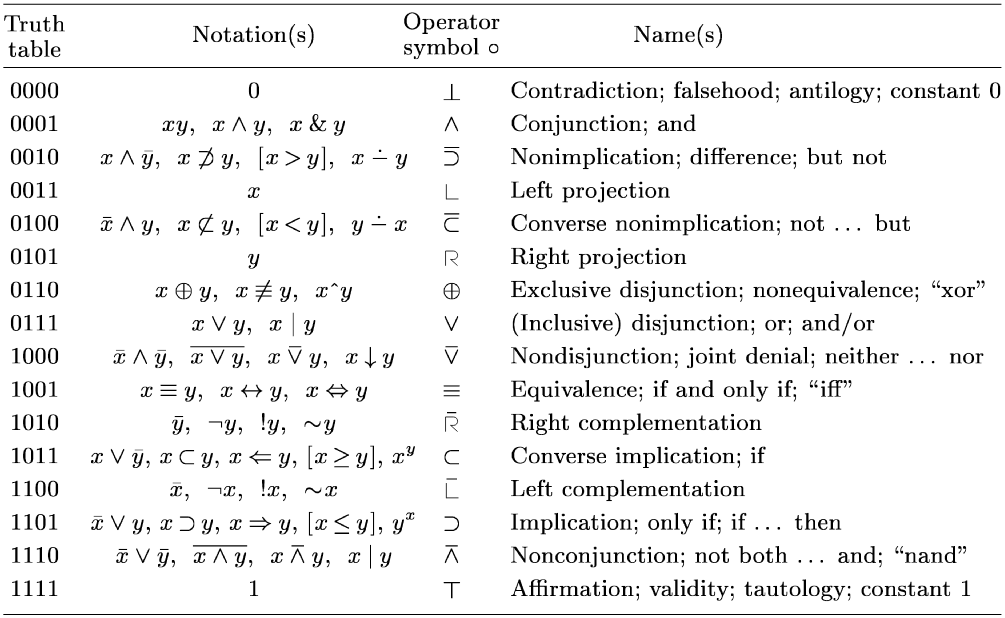
\includegraphics [width=5in]{TableOfPropositionalOperators}
   \caption{TableOfPropositionalOperators}
   \label{table:TableOfPropositionalOperators}
\end{table}

    \subsection {Boolean Expressions and Boolean Functions}

 \begin{table}[htbp]
   \centering
   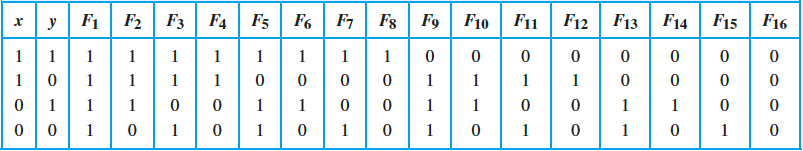
\includegraphics [width=5in]{Table-12-1-3-BooleanFunctionsOfTwoVariables}
   \caption{Table of Boolean Functions of Two Variables}
   \label{table:TableOfBooleanFunctionsOfTwoVariables}
\end{table}

    \subsection {Identities of Boolean Algebra}
    \subsection {Principle of Duality}
Note the similarity of Table 1.1 and 2.1. This is no accident but instead is a fundamental point that is explored in more detail in the math course, Abstract Algebra. One fact that should be noted is the Principle of Duality.

    \subsection {Abstract Definition of a Boolean Algebra}

\section {Representing Boolean Functions}
    \subsection {Sum-of-Products Expansions}
    \subsection {Functional Completeness}
    
\section {Logic Gates}

The logic of signals on wires can be made to obey the laws of logic. Some voltage is used to represent \textit{true} while another is used to represent \textit{false}. Electrical circuits have been created which implement the laws of the logical operators we have already seen and they are called \textit{gates}. We introduce two notations for representing this type of logic, one the visual one which is often seen in a circuits class and another that is a more algebraic notation.

	\begin{definition}[Logic gates]\index{logic gate}

\begin{figure}[htbp]
   \centering
   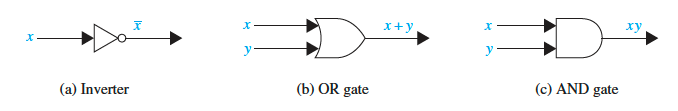
\includegraphics [width=5in]{Figure-12-3-1-BasicGates}
   \caption{Basic Logic Gages}
   \label{figure:BasicLogicGates}
\end{figure}
	\end{definition}

    \subsection {Combinations of Gates}
    \subsection {Adders}
    \subsection {Minimization of Circuits}
	\subsection {combinational circuits versus sequential circuits}
    \subsection {Karnaugh Maps and Quine-McCluskey Method}

Two meanings: one the notation used by Boole, the other the more general observation that this algebra is the same as for logic and sets. The general topic of other algebras is covered in a course on abstract algebra in the math department. 

Sum of Products form for Boolean Algebras
well formed formula
fundamental product
Algorithm for finding sum-of-products form
complete sum of products form, midterms, DNF

Homomorphism between Boolean Algebra and basic logic gates

	


                                                                                                  %%%%       GRAPHS           %%%

\chapter {Graphs}
vertices or nodes, edges (directed or undirected), head, tail, in-degree, out-degree, self-loop (reflexive), was covered in the chapter on functions.
Famous algorithms for graph traversal


\section {Graphs and Graph Models}
\begin{definition}[Graph]\index{graph}\index{vertex}\index{edge}
A \textit{graph} $G =(V,E)$ consistes of a non-empty set $V$ of \textit{vertices} or \textit{nodes} and $E$, a set of \textit{edges}. Each edge has either one or two vertices associated ith it, called its \textit{endpoints}. An edge is said to \textit{connect} its endpoints.
\end{definition}
\begin{notes}
The number of vertices does not need to be finite. But we will only discuss finite graphs in this outline.
\end{notes}

\begin {definition} [Simple Graph]\index{simple graph}
A graph in which each edge connects two different vertices and where no two edges connect the same pair of vertices is called a \textbf{simple graph}. The edge in a simple graph can be denoted by the set of vertices it connects.
\end{definition}

\begin {definition}[Multigraph]\index{multigraph}
Graphs that have multiple edges connecting the same vertices are called \textbf{multigraphs}. We say that each edge has a multiplicity of edges between the two vertices.
\end{definition}

\begin{definition}[Directed or Digraph]\index{directed graph}\index{digraph}
A \textit{directed graph} (or \textit{digraph} $(V,E)$ consists of a nonempty set of vertices $V$ and a set of \textit{directed edges} or \textit{arcs} $E$. Each directed edge is associated with an ordereed pair of vertices. The directed edge associated with the ordered pair $(u,v)$ is said to start with $u$ and end at $v$. When presented in a picture, the directed edge has an arrow that starts at the vertex $u$ and ends at $v$. A directed graph may also have multiple directed edges.
\end{definition}

Graphs model a great many applications in software engineering. They include Acuaintanceship Graphs, Influence Graphs, The Hollywood Graph, Round-Robin Tournaments, Collaboration Graphs, Road Maps, Call Graphs, and the WWW.

\section {Graph Terminology and Special Types of Graphs}
\begin{definition}[Edges in an Undirected Graph]
Two vertices $u$ and $v$ in an undirected graph $G$ are called \textit{adjacent} (or \textit{neighbors} in $G$ if $u$ and $v$ are endpoints of an edge of $G$. If $e$ is associated with $\{u,v\}$, the edge $e$ is called \textit{incident with} the vertices $u$ and $v$. The edge $e$ is also said to \textit{connect u} and \textit{v}. The vertices $u$ and $v$ ar called \textit{endpoints} of an edge associated with $\{u,v\}$.
\end{definition}

\begin{definition}
The \textit{degree of a vertex in an undirected graph} is the number of edges incident with it, except that a loop at a vertex contributes twice to the degree of that vertex. The degree of the vertex $v$ is denoted by deg($v$). A vertex of degree zero is called \textbf{isolated} while a vertex with degree one is called \textbf{pendant}
\end{definition}

\begin{theorem} [The Handshaking Theorem]\index{handshaking theorem}
Let $G=(V,E)$ be an undirected graph with $e$ edges. Then 
$$2e = \Sigma_{v\in V} deg(v)$$.
\end{theorem}
\begin{notes}
This is true even when multiple edges and loops are present.
\end{notes}

\begin{theorem}
An undirected graph has an even number of vertices of odd degree.
\end{theorem}

\begin{definition}
When $(u,v)$ is an edge of the graph $G$ with directed edges, $u$ is said to be \textit{adjacent to v} and $v$ is said to be \textit{adjacent from u}. The vertex $u$ is called the \textit{initial vertex} of $(u,v)$, and $v$ is called the \textit{terminal} or \textit{end vertex} of $(u,v)$. The initial and terminal vertex of a loop are the same.
\end{definition}

\begin{definition}
In a graph with directed edges, the \textit{in-degree of a vertex v}, denoted by $\text{deg}^-(v)$, is the number of edges with $v$ as their terminal vertex. The \textit{out-degree of v}, denoted by $\text{deg}^+(v)$, is the number of edges with $v$ as their initial vertex. (Note that a loop at a vertex constributes 1 to both the in-degree and the out-degree of this vertex.)
\end{definition}

\begin{theorem}
Let $G=(V,E)$ be a graph with directed edges. Then
$$\Sigma_{v\in V} \text{deg}^-(v) = \Sigma_{v \in V} \text{deg}^+(v) = \lvert E \rvert$$
\end{theorem}

\begin{definition}Here are the definitions of some common simple graphs:\\
A \textbf{Complete Graph on $n$-vertices} is a simple graph that contains exactly one edge between each pair of distinct vertices. It is denoted by $K_n$.\\
A \textbf{Cycle} of $n$ vertices, $n\ge3$, $v_1,v_2, \dots ,v_3$ has edges $\{v_1,v_2\},\{v_2,v_3\}, \dots ,\{v_{n-1},v_n\}, \{v_n,v_1\}$. It is denoted $C_n$.\\
A \textbf{Wheel} is created by taking a cycle, $C_n$, adding a single vertex $v$ and adding an edge from the new vertex $v$ to each of the $n$ existing vertices of the cycle. It is designated $W_n$.\\
The \textbf{$n$-dimensional hypercube} or \textbf{$n$-cube} is the graph that has vertices representing the $2^n$ bit strings of length ....blah blah
\end{definition}

\begin{definition}[Bipartite Graph]\index{bipartite graph}
A simple graph $G$ is called \textit{bipartite} if its vertex set $v$ can be partititoned into two disjoint sets $V_1$ and $V_2$ such that evry edge in the graph connects a vertex in $V_1$ and a vertex in $V_2$. For such a graph we call the pair $(V_1,V_2) $ a \textit{bipartition} set $V$ of $G$.
\end {definition}

\begin{theorem}
A simple graph is bipartte if an donly if it is possible to assign one of two different colors to each vertex of the graph so that no two adjacent vertices are assigned the same color. This is called a \textit{graph coloring}.
\end{theorem}

\begin{definition}[Complete Bipartite Graphs]
The \textbf{complete bipartite graph $K_{m,n}$} is the graph that has its vertex set partitioned into two subsets of $m$ and $n$  vertices, respectively. There is an edge between two vertices if and only if one vertex is in the first subset and the other vertex is in the second subset. 
\end{definition}

\begin{definition}
A \textit{subgraph of a graph} $G=(V,E)$ is a graph $H=(W,F)$, where $ W \subset V$ and $F \subset E$. A subgraph $H$ of $G$ is a \textit{proper subgraph} of $G$ if $H \neq G$.
\end{definition}

\begin{definition}
The \textit{union} of two simple graphs $G_1 = (V_1,E_1)$ and $G_2=(V_2,E_2)$ is the simple graph with vertext set $V_1 \cup V_2$ and edge set $E_1 \cup E_2$. The unions of $G_1$ and $G_2$ is denoted by $G_1 \cup G_2$.
\end{definition}


\section {Representing Graphs and Graph Isomorphism}
Sometimes we look at graphics that depict two different graphs but we see that while they look different we can make one match to the other by moving vertices around. This leads us to look at how we represent graphs and to define what we mean by saying two graphs are somehow the same.

There are two common way that graphs are represented using tables and these are useful in software engineering. We look at adjacency lists and adjacency matrices.

\begin{definition}
A simple graph $G$ can be represented by listing each vertex and the vertices that are adjacent to it. This is called an \textbf{adjacency list}. This can be extended to include a representation of directed graphs. Note that the size of the lists will be half the size of an undirected graph.
\end{definition}

\begin{definition}
A simple graph $G$ can be represented by a two dimensional matrix with the vertices of the graph on both axes. The presence of an edge between them can be represented by a value in the matrix. 

Suppose that $G=(V,E)$ is a simple graph where $\lvert V \rvert = n$. Suppose that the vertices of $G$ are listing arbitraryily as $v_1,v_2, \dots ,v_n$. The \textbf{adjacency matrix $A$} (or $A_G$) of $G$, with respect to this listing of the vertices, is the $n \times n$ zero-one matrix with 1 as its $(i,j)$th entry when $v_i$ and $v_j$ are adjacent, and 0 as its $(i,j)$th entry when they are not adjacnt. In other words, if its adacency matrix is $A=[a_{ij}]$, then 

cases

\end{definition}

\begin{definition}
Graphs can be represented by an \textbf{incidence matrix}. Let $G=(V,E)$ be an undirected graph. Suppose that $v_1,v_2, \dots ,v_n$ are the vertices and $e_1,e_2, \dots ,e_m$ are the edges of $G$. Then the incidence matrix with respect to this ordering of $V$ and $E$ is the $n \times n$ matrix $M=[i,j]$, where

cases
\end{definition}

\begin{definition}
The simple graphs $G_1=(V_1,E_1)$ and $G_2=(V_2,E_2)$ are \textit{isomorphic} if there is a one-to-one and onto function (a bijection) $f$ from $V_1$ to $V_2$ with the property that $a$ and $b$ are adjacent in $G_1$ if and only if $f(a)$ and $f(b)$ are adjacent in $G_2$, for all $a$ and $b$ in $V_1$. Such a function $f$ is called an \textit{isomorphism}.
\end{definition}

Worst case algorithms to determine graph isomorphism have exponential worst case time complexity. However there are algorithms that have linear average time complexity for graph isomorphism. 

\section {Connectivity}


\section {Euler Paths and Circuits}
  \begin{figure}[htbp]
   \centering
   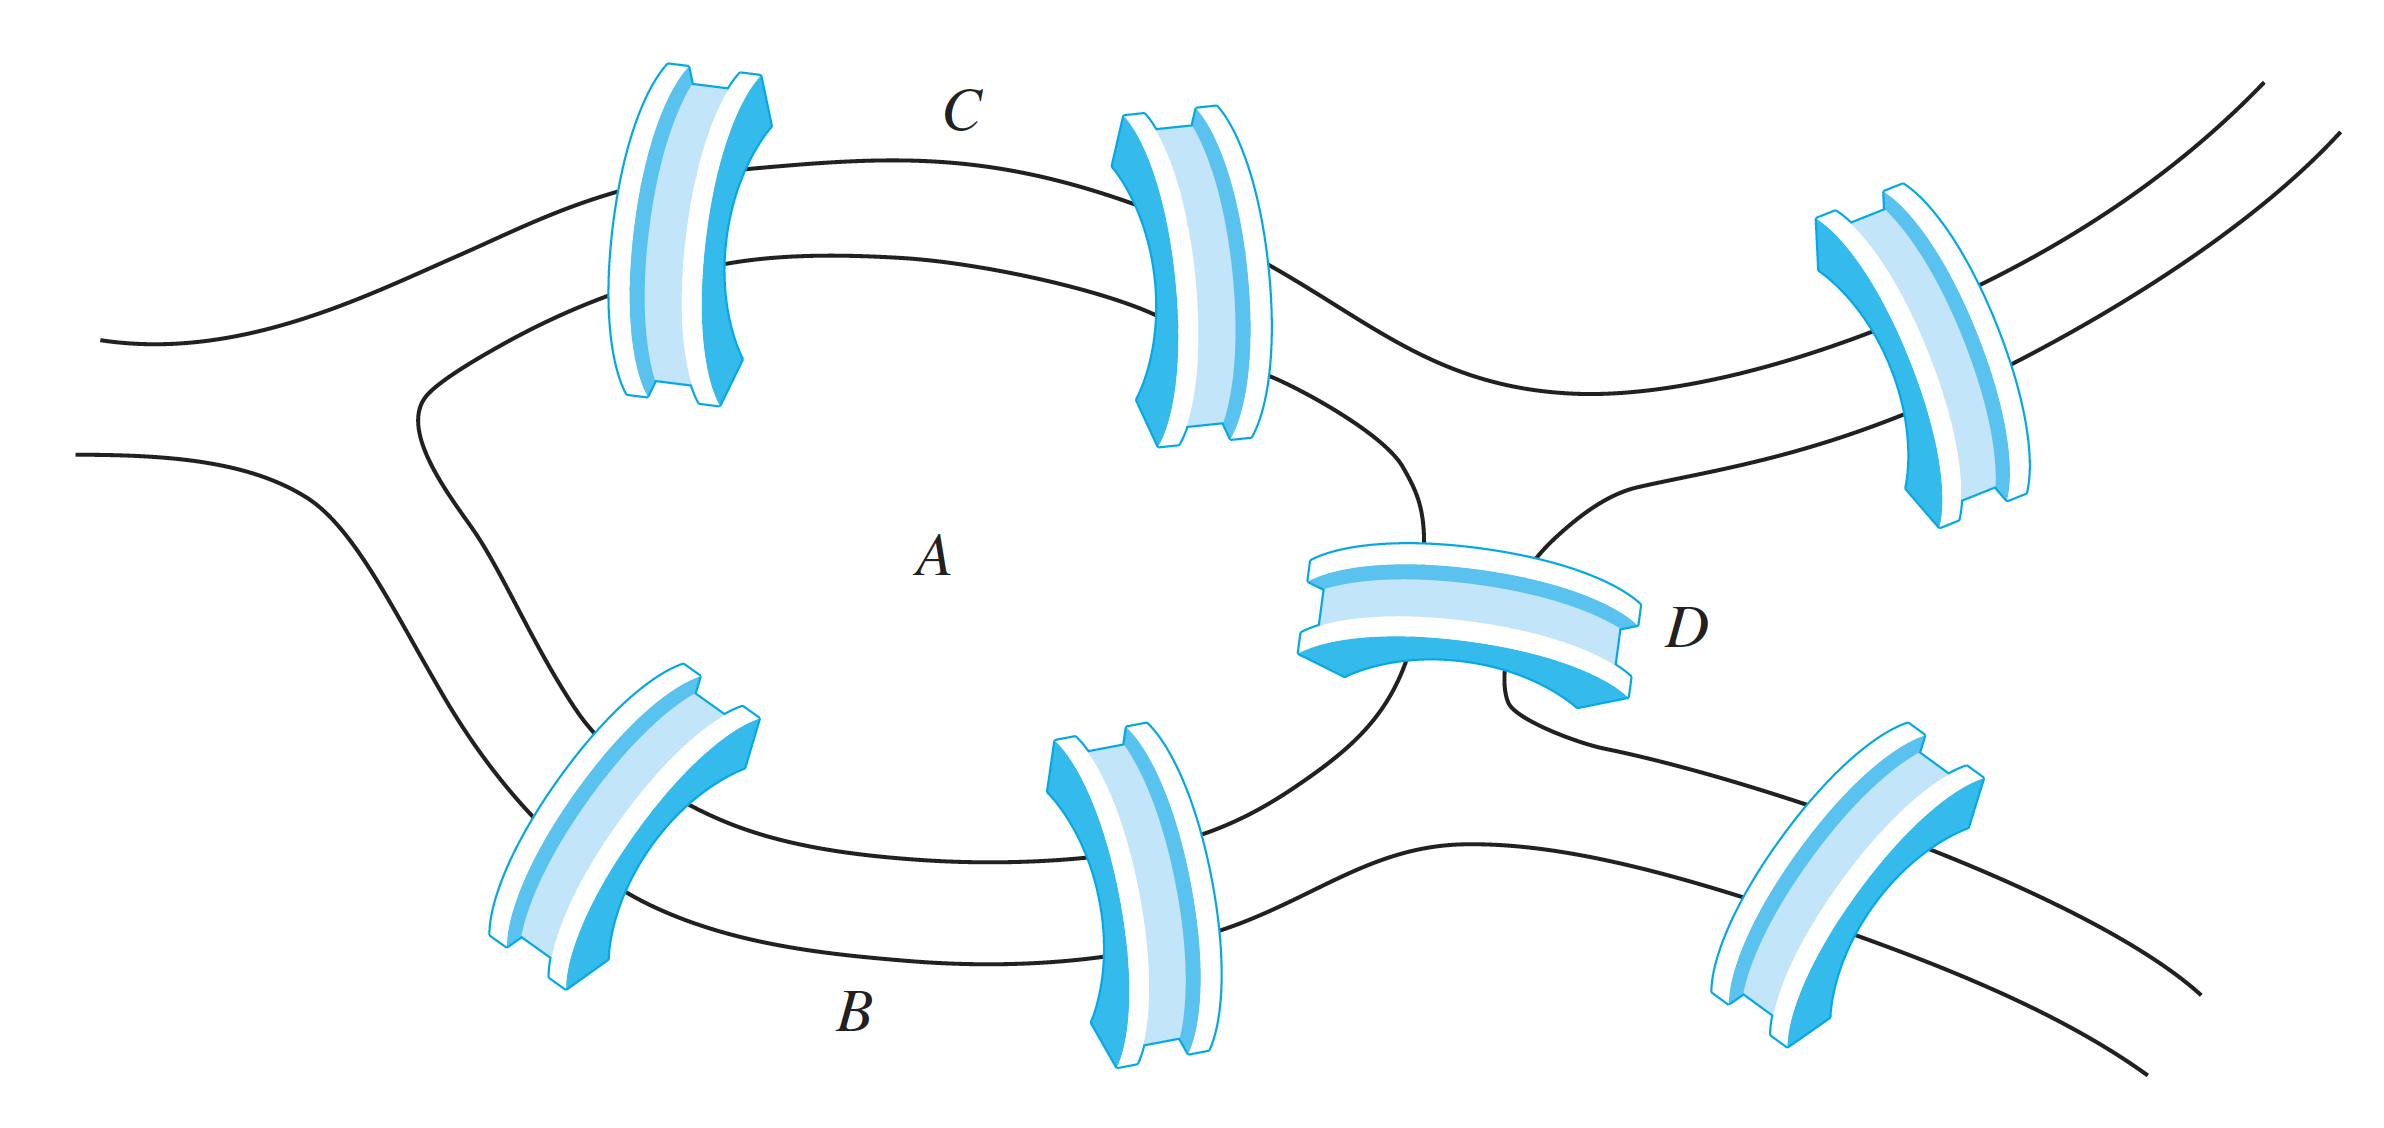
\includegraphics [width=5in]{Figure-10-6-1-BridgesOfKoenigsberg}
%figure from Rosen
   \caption{The Bridges of Koenigsberg}
   \label{figure:BridgesOfKoenigsberg}
\end{figure}

\begin{definition}
An \textit{Euler circuit} in a graph $G$ is a simple circuit containing every edge of $G$. An \textit{Euler path} in $G$ is a simple path containing every edge of $G$.
\end{definition}

\begin{theorem}
A connected multigraph with at least two vertices has an Euler curcuit if and only if each of its vertices has even degree.
\end{theorem}

NECESSARY AND SUFFICIENT CONDITIONS FOR EULER CIRCUITS AND PATHS
There are simple criteria for determining whether a multigraph has an Euler circuit or an Euler
path. Euler discovered them when he solved the famous Königsberg bridge problem. We will
assume that all graphs discussed in this section have a finite number of vertices and edges.
What can we say if a connected multigraph has an Euler circuit? What we can show is that
every vertex must have even degree. To do this, first note that an Euler circuit begins with a
vertex a and continues with an edge incident with a, say {a, b}. The edge {a, b} contributes one
to deg(a). Each time the circuit passes through a vertex it contributes two to the vertex’s degree,
because the circuit enters via an edge incident with this vertex and leaves via another such edge.
Finally, the circuit terminates where it started, contributing one to deg(a). Therefore, deg(a)
must be even, because the circuit contributes one when it begins, one when it ends, and two
every time it passes through a (if it ever does). A vertex other than a has even degree because
the circuit contributes two to its degree each time it passes through the vertex.We conclude that
if a connected graph has an Euler circuit, then every vertex must have even degree.
Is this necessary condition for the existence of an Euler circuit also sufficient? That is, must
an Euler circuit exist in a connected multigraph if all vertices have even degree? This question
can be settled affirmatively with a construction.

Algorithm: Constructing Euler Circuits

\begin{theorem}
A connected multigraph has an Euler path but not an Euler circuit if and only if it has exactly two vertices of odd degree.
\end{theorem}
\section{Hamilton Paths and Circuits}
\begin{definition}
A simple path in a graph $G$ that passes through every vertex exactly once is called a \textit{Hamilton path}, and a simple circuit in graph $G$ that passes through everty vertex exactly once is called a \textit{Hamilton circuit}. That is, the simple path $x_0,x_1,\dots ,x_{n-1},x_n$ and $x_i\neq x_j$ for $0 \le i  < j \le n$, and the simple circuit $x_0,x_1, \dots ,x_{n-1},x_n,x_0$ (with $n>0$) is a Hamilton circuit if $x_0,x_1, \dots x_{n-1},x_n$ is a Hamilton path.
\end{definition}
CONDITIONS FORTHE EXISTENCE OF HAMILTON CIRCUITS Is there a simple way
to determine whether a graph has a Hamilton circuit or path? At first, it might seem that there
should be an easy way to determine this, because there is a simple way to answer the similar
question of whether a graph has an Euler circuit. Surprisingly, there are no known simple
necessary and sufficient criteria for the existence of Hamilton circuits. However, many theorems
are known that give sufficient conditions for the existence of Hamilton circuits. Also, certain
properties can be used to show that a graph has no Hamilton circuit. For instance, a graph with a
vertex of degree one cannot have a Hamilton circuit, because in a Hamilton circuit, each vertex
is incident with two edges in the circuit. Moreover, if a vertex in the graph has degree two, then
both edges that are incident with this vertex must be part of any Hamilton circuit. Also, note
that when a Hamilton circuit is being constructed and this circuit has passed through a vertex,
then all remaining edges incident with this vertex, other than the two used in the circuit, can be
removed from consideration. Furthermore, a Hamilton circuit cannot contain a smaller circuit
within it.

\begin{theorem}[Dirac's Theorem]
If $G$ is a simple graph with $n$ vertices with $n \ge 3$ such that the degree of every vertex in $G$ is at least $\frac{n}{2}$, then $G$ has a Hamilton circuit.
\end{theorem}

\begin{theorem}[Ore's Theorem]
If $G$ is a simple graph with $n$ vertices with $n \ge 3$ such that deg($u$)+deg($v$) $\ge n$ for every pair of nonadjacent vertices $u$ and $v$ in $G$, then $G$ has a Hamilton circuit.
\end{theorem}

\section {Shortest Path Problem}
Dijkstra's Algorithm

\begin{theorem}
Dijkstra's algorithm finds the length of a shortest path between two vertices in a connected simple undirected weighted graph.
\end{theorem}

\begin{theorem}
Dijkstra's algorithm uses $O(n^2)$ operations (additions and comparisons) to find the length of a shortest path between two vertices in a connected siple undirected weighted graph with $n$ vertices.
\end{theorem}

\begin{figure}[htbp]
   \centering
   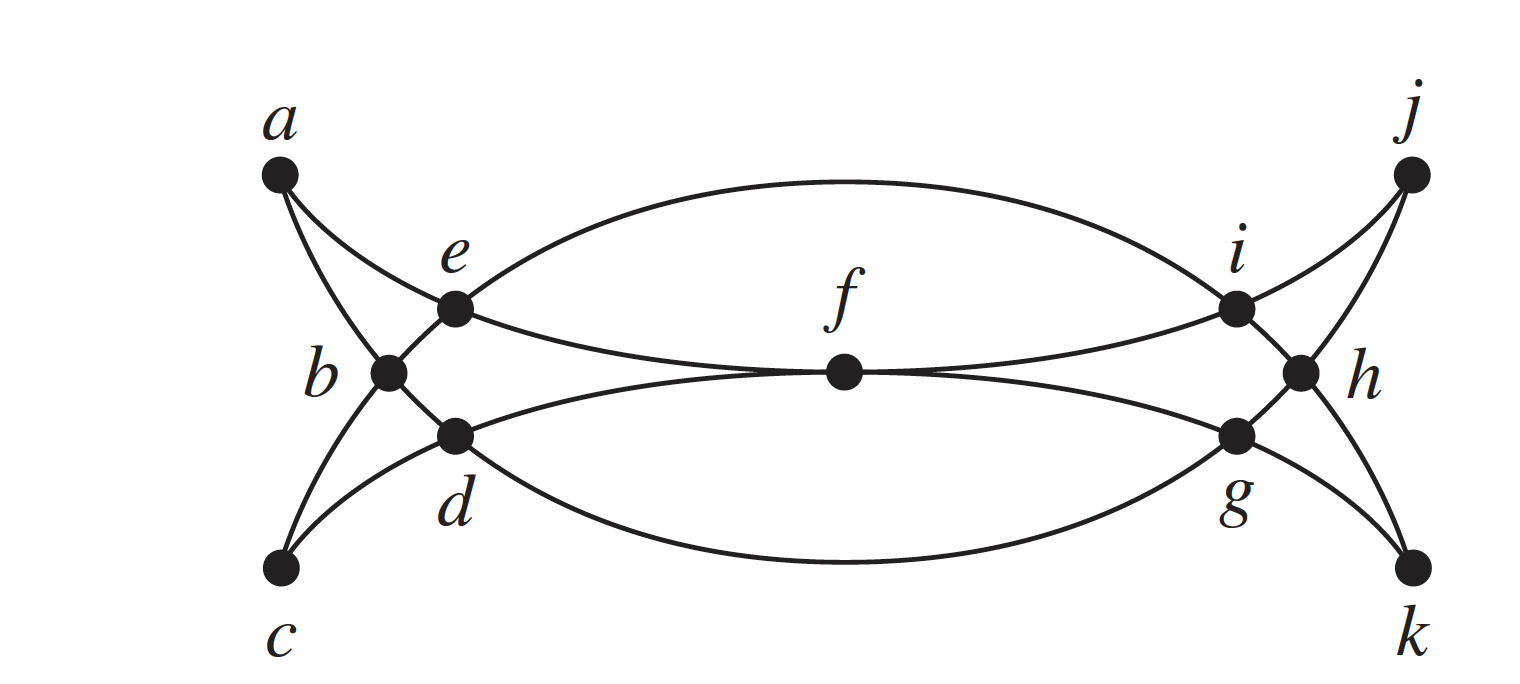
\includegraphics [width=3in]{Figure-10-5-6-MohammedsScimitar}
   \caption{Mohammeds Scimitar}
   \label{figure:Figure-10-5-6-MohammedsScimitar}
\end{figure}

\section {Planar Graphs}
\begin{definition}
A graph is called \textit{planar} if it can be drawn in the plane without any edges crossing (where a crossing of edges is the intersection of the lines or arcs represening them at a point other than their common endpoint). Such a drawing is called a \textit{planar representation} of the graph.
\end{definition}

\begin{theorem}[Euler's Formula]
Let $G$ be a connected planar simple graph with $e$ edges and $v$ vertices. Let $r$ be the number of regions in a planar representation of $G$. Then $r-e-v+2$.
\end{theorem}

\begin{corollary}
If $G$ is a connected planar simple graph with $e$ edges and $v$ vertices, where $v \ge 3$, then $e \le 3v -  6$
\end{corollary}

\begin{corollary}
If $G$ is a connected planar simple, graph then $G$ has a vertex of degree not exceeding five.
\end{corollary}

\begin{corollary}
If a connected planar simple graph has $e$edges and $v$ vertices with $v \ge 3$ and no circuits of length three, then $e \le 2v - 4$.
\end{corollary}

\begin{theorem}
A graph is nonplanar if and only if it contains a subgraph homeomorphic to $K_{3,3}$ or $K_5$.
\end{theorem}

\section {Graph Coloring}
\begin{definition}
A \textit{coloring} of a simple graph is the assignment of  acolor to each vertex of the graph so that no two adjacent vertices are assigned the same color.
\end{definition}

\begin{definition}
The \textit{chromatic number} of a graph is the least number of colors needed for a coloring of this graph. The chromatic number of a graph $G$ is denoted by $\chi(G)$ (where $\chi$ is the Greek letter chi).
\end{definition}

\begin{theorem}[The Four Color Theorem]
The chromatic number of a planar graph is no greater than four.
\end{theorem}

\newpage
	


                                                                            %%%%%%%%%%%    TREES    %%%
\chapter {Trees}
Recursive def of trees, some famous algorithms for trees

\begin{definition}[Tree]
A \textit{tree} is a connected undirected graph with no simple circuits.
\end{definition}

\begin{theorem}
An undirected graph is a tree if and only if there is a unique simple path between any two of its vertices.
\end{theorem}

\begin{definition}[Rooted Tree]
A \textit{rooted tree} is a tree in hwich one vertex has been designated as the root and every edge is directed away from the root. Suppose $T$ is a rooted tree. If $v$ is a vertex in $T$ other than the root, the \textbf{parent} of $v$ is the unique vertex $u$ such that there is a directed edge from $u$ to $v$. When $u$ is the parent of $v$, $v$ is called a \textbf{child} of $u$. Vertices with the same parent are called \textbf{siblings}. The \textbf{ancestors} of a vertex other than the root are the vertices in the path from the root to this vertex, excluding the vertex itself but including the root. The \textbf{descendants} of a vertex $v$ are those vetices that have $v$ as an ancestor. A vertex of a tree is called a \textbf{leaf} if it has no children. Vertices that have children are called \textbf{internal vertices}. The root is an internal vertex unless it is the only vertex in the graph, in which case it is a leaf. If $a$ is a vertexin a tree, the \textbf{subtree} with $a$ as its root is the subgraph of the tree consisting of $a$ and its descendants and all edges incident to those descendants.
\end{definition}

\begin{definition}
A rooted tree is called an \textit{m-ary tree} if every internal vertex has no more than $m$ children. The tree is called a "\textit{full m-ary tree}" if every internal vertex has exactly $m$ children. An \textit{m}-ary tree with $m=2$ is called an \textit{binary tree}. 
\end{definition} 

\begin{definition}
An \textbf{ordered rooted tree} is a rooted tree where the children of each internal vertex are ordered. Orered rooted trees are drawn so that the hcildren of each internal vertex are shown in order from left to right. Note that a representation of a rooted tree in the conventional way determines an ordering for its edges. 

In an orderedf binary tree (usually called a \textbf{binary tree}), if an internal vertex has two children, the first child is called the \textbf{left child} and the second child is called the \textbf{right child}. The tree rooted at the left child of a vertex is called the \textbf{left subtree} of this vertex, and the tree rooted at the right child of a vertex is called the \textbf{right subtree} of the vertex. 
\end{definition}

\section{Properties of Trees}

\begin{theorem}
A tree with $n$ vertices has $n-1$ edges.
\end{theorem}

\begin{theorem}
A full $m$-ary tree with $i$ internal vertices contains $n=mi+1$ vertices.
\end{theorem}

\begin{theorem}
A full $m$-ary tree with 
\begin{enumerate}[label=(\roman*)]
  \item $n$ vertices has $i=(n-1)/m$ internal vertices and $l=[(m-1)n+1]/m$ leaves,
  \item $i$ internal vertices has $n=mi+1$ vertices and $l=(m-1)i+1$ leaves,
  \item $l$ leaves have $n=(ml-1)/(m-1)$ vertices and $i=(l-1)(m-1)$ internal vertices.
\end{enumerate}
\end{theorem}

\begin{definition}
The level of a vertex $v$ in a rooted tree is the length of the unique path from the root to this vertex. The level of the root is defined to be zero. The \textbf{height} of a rooted tree is the maximum of the levels of vertices. In other words, the height of a rooted tree is the length of the longest path from the root to any vertex. A rooted $m$-ary tree of hgitht $h$ is \textbf{balanced} if all leaves are at levels $h$ or $h-1$.
\end{definition}

\begin{theorem}
There are at most $m^h$ leaves in an $m$-ary tree of height $h$.
\end{theorem}

\begin{corollary}
If an $m$-ary tree of height $h$ has $l$ leaves, then $h \ge \lceil \log_ml \rceil$. If the $m$-ary tree is full and balanced, then $h= \lceil \log_ml \rceil$ 
\end{corollary}

\newpage



	



                %%%   PROBABILITY   %%%
\chapter {Discrete Probability}
\section {An Introduction to Discrete Probability}
    \subsection {Finite Probability}
    \subsection {The Probability of Combinations of Events}
    \subsection {Probabilistic Reasoning}

\section {Probability Theory}
    \subsection {Assigning Probabilities}
    \subsection {Combinations of Events}
    \subsection {Conditional Probability}
    \subsection {Independence}
    \subsection {Bernoulli Trials and the Binomial Distrubution}
    \subsection {The Birthday Problem}
    \subsection {Monte Carlo Algorithms}
    \subsection {The Probabilistic Method}






Let p be the proposition that the sum of the first n odd numbers is n**2. How can we prove such a proposition? Here is the example of how inductive reasoning works. 

We can easily evaluate this proposition for small values of n and see that they are true. But since the set of input values is the set of natural numbers we cannot do this for all elements of the set. So we observe this, let us assume that this proposition is true for some value k which is bigger than any value we evaluated manually. If we can prove that the statement MUST be true for the next value, the successor of k, k+1, then we have proven that it must be true for ALL values of n drawn from the natural numbers since we know it is true for the small values and we can continually apply the reasoning that got us from k to k+1 as many times as we need to give us all the values to infinity.

So first we introduce the inductive hypothesis, that it is true for some k:
Assume that the first k odd numbers sum to k**2. Now we have the proof obligation to prove that with that assumption that this MUST be true for k+1, that is, the sum of the first k+1 odd numbers will give us (k+1)**2. This requires some clever algebra but nothing you can't follow:

the first k odd number sum to k**2
Sigma(i=0 to k, 2i+1) = Sigma(i=1 to k-1, 2i+1) = k**2
which is equivalent to 
1+3+5+ ... +2(k-1) = k**2
we add 2(k+1) to both sides of the equation giving
1+3+5+ ... +2(k-1)+2(k+1) = (k+1)**2 = (k**2 + 2k + 1)=k**2 + (2k+1)
Using the premise, we rewrite the LHS
1+3+5+ ... +2(k-1)  + 2(k+1) = k**2 + 2(k+1)= k**2 + 2k + 1
showing the left and RHS of the equation are equal QED.

The general principle of weak form of mathematical induction is
First, show the proposition is true for one small element from the input.
Show that IF the proposition is true for some arbitrary k, that it MUST also be true for the next value after k, k+1. 
After both parts are proven, you have proven for all value from N.

CAUTION: The inductive assumption looks similar to the thing to be proven but you may not use that in the argument. You must use an arbitrary value k, and then prove that it must also be true for k+1 without again stating the assumption. To do so is the famous logical fallacy of assuming the antecedent or begging the question. This is a common error in inductive proofs.

There are a set of proofs that can be solved inductively but require that more than one small value be proven. This leads to the stronger form of inductive reasoning. In the strong form, you must prove that the proposition holds for some small number of values.

Open Form versus Closed Form Solutions
Note that we have proved an equivalence between two expressions, the sum of the first n odd numbers and the expression n**2. The first form has the implied algorithm of summing the first n odd integers, something that is of O(n) while the second has O(1). We call the first version an open form solution while we call the second a closed form solution. The computational advantage is obvious.

\newpage
	

           %%% COMPUTATION and FORMAL LANGUAGES  %%%
                                                                 
% This chapter can be skipped for programs that require a Theory of Computation Course that does not have a prerequisite
(Excluded from UCD course offerings)
\chapter {Computation}
Association between Automata, Grammar, Language. Difference between syntax and semantics in natural language. Object first or object last in natural language. 

\section {Languages and Grammars}
We saw that the notation $A_*$ designates all the possible strings that can be constructed from the set $A$. When the set A contains symbols that are distinguishable from each other we call that set an $\textit{alphabet}$ and refer to it with the greek letter $\Sigma$. Since there is no ambiguity between the strings $(a_1,a_2, \dots a_n)$ and $a_1a_2a_3 \dots a_n$ for strings of length $n$, we adopt this notation for string sequences. For short strings then
$$(w,o,r,d) = word$$
We call such strings words, the symbols from the alphabet lettersand the finite sequences in $\Sigma_*$ as the strings or words generated by the letters of $\Sigma$.

Alphabet, Words
Operations on words: concatenation
Formal Definition of Language
Operations on Languages
    \subsection {Phrase-Structured Grammars}
Regular Expressions, Regular Languages
Generative Grammars, Rules of Production
    \subsection {Context Free and Context Sensitive Grammars}
    \subsection {Regular Languages and their Notation}
    \subsection {Derivation Trees}
    parsing
    \subsection {Backus-Naur Form}
    
\section {Finite State Machines}
States, State Transition, Finite State Automata
    \subsection {FSM with no output}
        \subsubsection {Set of Strings}
        \subsubsection {Finite-State Automata}
        Def 3: A \textit{finite-state automata} $M=(S,I,f,s_0,F)$ consists of a finite set $S$ of \textit{states}, a finite \textit{input alphabet} $I$, a \textit{transition function} $f$ that assigns a next state to every pair of state and input (so that $f:S \times I \rightarrow S$, an \textit{initial} or \textit{start state} $s_0$, and a subset $F$ of $S$ consisting of \textit{final} (or \textit{accepting states}.
        
        \subsubsection {Language Recognition by FSA}
        \subsubsection {Non-deterministic FSA}
        
    \subsection {FSM with output}
    Mealy and Moore machines
    
\section {Language Recognition}
    \subsection {Regular Sets}
    \subsection {Kleene's Theorem}
    \subsection {Regular Sets and Regular Grammars}
    \subsection {Beyond Regular Languages and FSMs}
A later class will explore grammars beyond regular grammars, the languages they generate and the automata that recognize them.


how do i do a citation? %\cite{Rosen:2002:DMA:579402}


\newpage
	
  \backmatter
	\printindex
	\bibliographystyle{unsrt}
	\bibliography{aspnes}
  
%%%%%%%%%%%%%%%%%%%%%%%%%%%%%%
\end{document}
